%%%%%%%% ICML 2025 EXAMPLE LATEX SUBMISSION FILE %%%%%%%%%%%%%%%%%

\documentclass{article}

% Recommended, but optional, packages for figures and better typesetting:
\usepackage{microtype}
\usepackage{graphicx}
\usepackage{subcaption}
\usepackage{caption}
\usepackage{rotating}
\usepackage{booktabs} % for professional tables

% hyperref makes hyperlinks in the resulting PDF.
% If your build breaks (sometimes temporarily if a hyperlink spans a page)
% please comment out the following usepackage line and replace
% \usepackage{icml2025} with \usepackage[nohyperref]{icml2025} above.
\usepackage{hyperref}


% Attempt to make hyperref and algorithmic work together better:
\newcommand{\theHalgorithm}{\arabic{algorithm}}

% Use the following line for the initial blind version submitted for review:
\usepackage{icml2025}

% If accepted, instead use the following line for the camera-ready submission:
% \usepackage[accepted]{icml2025}

% For theorems and such
\usepackage{amsmath}
\usepackage{amssymb}
\usepackage{mathtools}
\usepackage{amsthm}

% if you use cleveref..
\usepackage[capitalize,noabbrev]{cleveref}

%%%%%%%%%%%%%%%%%%%%%%%%%%%%%%%%
% THEOREMS
%%%%%%%%%%%%%%%%%%%%%%%%%%%%%%%%
\theoremstyle{plain}
\newtheorem{theorem}{Theorem}[section]
\newtheorem{proposition}[theorem]{Proposition}
\newtheorem{lemma}[theorem]{Lemma}
\newtheorem{corollary}[theorem]{Corollary}
\theoremstyle{definition}
\newtheorem{definition}[theorem]{Definition}
\newtheorem{assumption}[theorem]{Assumption}
\theoremstyle{remark}
\newtheorem{remark}[theorem]{Remark}

% Todonotes is useful during development; simply uncomment the next line
%    and comment out the line below the next line to turn off comments
%\usepackage[disable,textsize=tiny]{todonotes}
\usepackage[textsize=tiny]{todonotes}


% The \icmltitle you define below is probably too long as a header.
% Therefore, a short form for the running title is supplied here:
\icmltitlerunning{Submission and Formatting Instructions for ICML 2025}

\begin{document}

\twocolumn[
\icmltitle{Degree of Staleness aware \\
           International Conference on Machine Learning (ICML 2025)}

% It is OKAY to include author information, even for blind
% submissions: the style file will automatically remove it for you
% unless you've provided the [accepted] option to the icml2025
% package.

% List of affiliations: The first argument should be a (short)
% identifier you will use later to specify author affiliations
% Academic affiliations should list Department, University, City, Region, Country
% Industry affiliations should list Company, City, Region, Country

% You can specify symbols, otherwise they are numbered in order.
% Ideally, you should not use this facility. Affiliations will be numbered
% in order of appearance and this is the preferred way.
\icmlsetsymbol{equal}{*}

\begin{icmlauthorlist}
\icmlauthor{Firstname1 Lastname1}{equal,yyy}
\icmlauthor{Firstname2 Lastname2}{equal,yyy,comp}
\icmlauthor{Firstname3 Lastname3}{comp}
\icmlauthor{Firstname4 Lastname4}{sch}
\icmlauthor{Firstname5 Lastname5}{yyy}
\icmlauthor{Firstname6 Lastname6}{sch,yyy,comp}
\icmlauthor{Firstname7 Lastname7}{comp}
%\icmlauthor{}{sch}
\icmlauthor{Firstname8 Lastname8}{sch}
\icmlauthor{Firstname8 Lastname8}{yyy,comp}
%\icmlauthor{}{sch}
%\icmlauthor{}{sch}
\end{icmlauthorlist}

\icmlaffiliation{yyy}{Department of XXX, University of YYY, Location, Country}
\icmlaffiliation{comp}{Company Name, Location, Country}
\icmlaffiliation{sch}{School of ZZZ, Institute of WWW, Location, Country}

\icmlcorrespondingauthor{Firstname1 Lastname1}{first1.last1@xxx.edu}
\icmlcorrespondingauthor{Firstname2 Lastname2}{first2.last2@www.uk}

% You may provide any keywords that you
% find helpful for describing your paper; these are used to populate
% the "keywords" metadata in the PDF but will not be shown in the document
\icmlkeywords{Machine Learning, ICML}

\vskip 0.3in
]

% this must go after the closing bracket ] following \twocolumn[ ...

% This command actually creates the footnote in the first column
% listing the affiliations and the copyright notice.
% The command takes one argument, which is text to display at the start of the footnote.
% The \icmlEqualContribution command is standard text for equal contribution.
% Remove it (just {}) if you do not need this facility.

%\printAffiliationsAndNotice{}  % leave blank if no need to mention equal contribution
\printAffiliationsAndNotice{\icmlEqualContribution} % otherwise use the standard text.

\begin{abstract}
Handling data staleness still remains a significant challenge in federated learning with highly time-sensitive tasks, where data are generated continuously and data staleness largely depends on timeliness of data.
Although recent works attempt to optimize data staleness by determining local data update frequency or client selection strategy with economic concern, none of them explore to take both data staleness and data volume into consideration.
In this paper, we introduce a novel metric, \textit{the Degree of Staleness (DoS)}, to quantify data staleness.
Based on this metric, we propose \textit{FedStream}, a DoS-aware incentive mechanism featuring an innovative local data update scheme manipulated by three knobs: the server's payment, outdated data conservation rate, and clients' fresh data collection volume, to coordinate staleness and volume of local data for best utilities.
We model this mechanism as a two-stage Stackelberg game with dynamic constraint, afterward deriving the dynamic optimal strategies for clients in close form and the approximately optimal strategy for the server.
Experimental results on real-world datasets demonstrates the significant performance of our approach.

\end{abstract}

\section{Introduction}
\label{Introduction}
With the development of Internet of Things(IoT), many end devices are generating plenty of data each day.
Due to the growing storage and computing power, it becomes more appealing to store data locally and push more compution function to them.
It motivates the application of federated learning, which supports local storage and local training on each device without violating their privacy.

A federated learning system comprises a parameter server and a large number of clients(i.e. end devices).
The server maintains a global model while each client owns local statistic.
During each iteration, clients download global model from the central server and makes local updates on their private data. Then the server will aggregate the updated models from the clients and generate a new global model.
The training process will terminate when the accuracy of global model has reached the preset threshold.
During the process, since clients share not their private data but the trained local model with the server, the federated learning system can protect clients' privacy efficiently.

Despite various advantages in enabling edge computing while protecting data privacy, it still faces two bottlenecks:
1) \textit{Staleness of Data:} In most existing works, clients are assumed to hold a static dataset and use the same dataset to train local model over the time horizon.
But in reality, there are many highly time-sensitive tasks with streaming data. That is, data are generated continuously and data valuation largely depends on timeliness of data \cite{xiao2023aoi}.
Under this circumstance, outdated data used for training may deteriorate model parameters and reduce model service quality.
2) \textit{Incentive Mechanism:} Incentive mechanism is attached great importance for stimulting clients to participate the training task. That's because clients consume various resources including computing capacity, communication bandwidth and battery charge while training.
Besides, collecting fresh data frequently to meet the requirement of highly time-sensitive tasks also cause extra cost. Considering huge resource expenditure, clients may be not reluctant to provide fresh data or even reject to participate in federated learning tasks without economic compensation.

Efforts have been made in incentive mechanism design ranging from game theory \cite{lim2020hierarchical} \cite{zhang2022enabling} \cite{huang2024collaboration} to auction theory \cite{jiao2020toward} and contract theory \cite{kang2019incentive} \cite{ding2020optimal}. However, most of these studies don't take into consideration the negative impact of outdated data on model performance.
A few works have studied AoI-concerned incentive mechanisms against mobile crowdsensing \cite{xiao2023aoi} \cite{wang2021taming}. But they can't be applied in the context of federated learning directly.
In the federated learning field, some papers discuss the AoI-concerned incentive mechanism, focusing on controlling dynamic prices or update frequency \cite{wang2019dynamic} \cite{wu2023towards}. But none of them explore to manipulate local data update by decaying stale data and collecting new data simultaneously considering value and volume of present data. 

Motivated by the above considerations, we introduce a novel metric: degree of staleness (DoS) to measure data value, based on which we propose a DoS-aware incentive mechanism in federated learning, called FedStream.
Different from previous works, this system allows the server to manipulate clients' local data update by launching monetary payment and enforced order at the same time according to DoS and data volume.
Specifically, the server controls two variables: payment intented to encourage clients to collect new data and conservation rate intented to force clients to abandon outdated data. It targets to minimize model accuracy loss with plenty of fresh data and as low monetary payment as possible.
For a particular client, it controls the volume of new data collected from local data stream dynamically according to the server's strategy. Before each communication round, it updates loal dataset by abandoning parts of outdated data as the server required and collecting some new data according to its own optimal strategy, then followed by local training. The objective of a client is to maximize the balance between payment related to its contribution share and various costs.

There are three key challenges in FedStream as follows.
First, the server faces a two-variable optimization problem in an complicated form. Besides, the client faces a long-term optimization problem with dynamic constraint of update strategy. How to derive the optimal strategy for both server and clients to maximize their utility is of significance and challenging.
Second, capturing the converged model performance before training is an important step to determine the optimal strategy of server. Intuitively, global model performance can be impacted by data volume and data staleness simultaneously. Specially, more fresh data will lead to better model performance, particularly in highly time-sensitive tasks. However, there is lack of quantitative relationship between global model performance and the freshness of data.
Third, to derive clients' optimal strategies, they need to estimate their expected benefit before training, which depends on reward by the server and respective contributed share. However, in many real-world scenarios, the contributed share is unknown since clients cannot communicate with each other. Unknown information makes it challenging to make decision on client side.

To overcome the above challenges, we first derive the convergence upper bound of FedStream for the server, which reveals the relationship between converged model performance and data staleness.
In addition, we introduce a mean-field term to estimate the unknown information for clients.
Based on the above two approaches, the optimization problems on both server and client side can be constructed respectively.
Then we use a Stackelberg game to model the interaction between both sides, where the server acts as a leader and clients are regarded as followers.
Lastly, with the aid of backward reduction approach, we derive the optimal solution for this Stackelberg game.

The main contributions in this paper are summarized as follows:
\begin{itemize}
  \item We propose a DoS-aware new federated learning system with the local data update scheme at the core. To fit the proposed update scheme, we define a novel concept of DoS to measure the degree of data staleness. Based on the definition, we conduct convergence analysis and secure the upper bound of converged upper bound for FedStream.
  \item On the basis of convergence upper bound, we construct the optimization problems for both the server and clients, where the server controls reward and conservation rate to minimize total cost, and clients control volume of new data to maximize their balance.
  \item We model the interaction between the server and clients as a Stackelberg game. Under the backward reduction, we derive clients' optimal strategy with Hamilton equation. Based on this ,we dervie the server's strategy by adopting a search algorithm.
  \item We carry out extensive experiments on two dataset: MNIST and FMNIST, to illustrate the extraordinary performance of FedStream.
\end{itemize}
The remainder of the paper is organized as follows: In Section 2, we introduce related work. We provide problem formulation and corresponding convergence analysis in Section 3. System model and methodology are demonstrated in Section 4 and 5 respectively. Then we conduct experiments in Section 6. The paper is concluded in Section 7.
Proofs of theorems and remarks are moved to the Appendix.

\section{Related Work}
\label{Related Work}
\subsection{Incentive Mechanism}
Incentive mechanism designed for federated learning has been widely investigated in previous works.
They can be assorted into three catagories:
(1) \textit{game theory:} 
\cite{lim2020hierarchical}  proposes a hierarchical incentive mechanism based on coalitional game theory approach, where multiple workers can form various federations.
\cite{zhang2022enabling} builds a incentive mechanism utilizing repeated game theory to enable long-term cooperation among participants in cross-silo federated learning.
\cite{huang2024collaboration} designs a novel incentive framework based on Stackelberg game to model the collaboration behaviour among server and clients in federated learning with difference privacy.
(2) \textit{auction theory:} 
\cite{jiao2020toward} designs two auction mechanisms for the federated learning platform to maximize the social welfare of the federated learning services market.
(3) \textit{contract theory:} 
\cite{kang2019incentive} proposes an effective incentive mechanism combining reputation with contract theory to motivate high-reputation mobile devices with high-quality data to participate in model learning.
\cite{ding2020optimal} presents an analytical study on the server's optimal incentive mechanism design by contract theory, in the presence of users' multi-dimensional private information.
However, the above studies don't take into consideration the negative impact of outdated data on model performance and they can't be applied in highly time-sensitive tasks.

\subsection{Data Staleness Optimization}
Many efforts have been devoted to data staleness optimization.
For example, \cite{tripathi2021age} consider the problem of minimizing age of information in general single-hop and multihop wireless networks.
\cite{fang2021computing} devises a joint preprocessing and transmission policy to minimize the average AoI and the energy consumption at the IoT device.
Only a few works among them study the AoI optimization with economic consideration. For example, \cite{xiao2023aoi} investigates the incentive mechanism design in MCS systems that take the freshness of collected data and social benefits into concerns.
\cite{wang2021taming} considers a general multi-period status acquisition system, aiming to maximize the aggregate social welfare and ensure the platform freshness.
However, they can't be applied in the context of federated learning.
In the federated learning field, \cite{wang2019dynamic} proposes dynamic pricing for the server to offer age-dependent monetary returns and encourages clients to sample information at different rates over time.
\cite{wu2023towards} aims to minimize the loss of global model for FL with a limited budget by determining a client selection strategy under time-sensitive scenarios.
But none of them explore to manipulate local data update by decaying stale data and collecting new data simultaneously considering value and volume of present data. 

\section{Problem Formulation}
\subsection{Federated Learning with Data Stream}
\begin{figure}[ht]
  \centering
  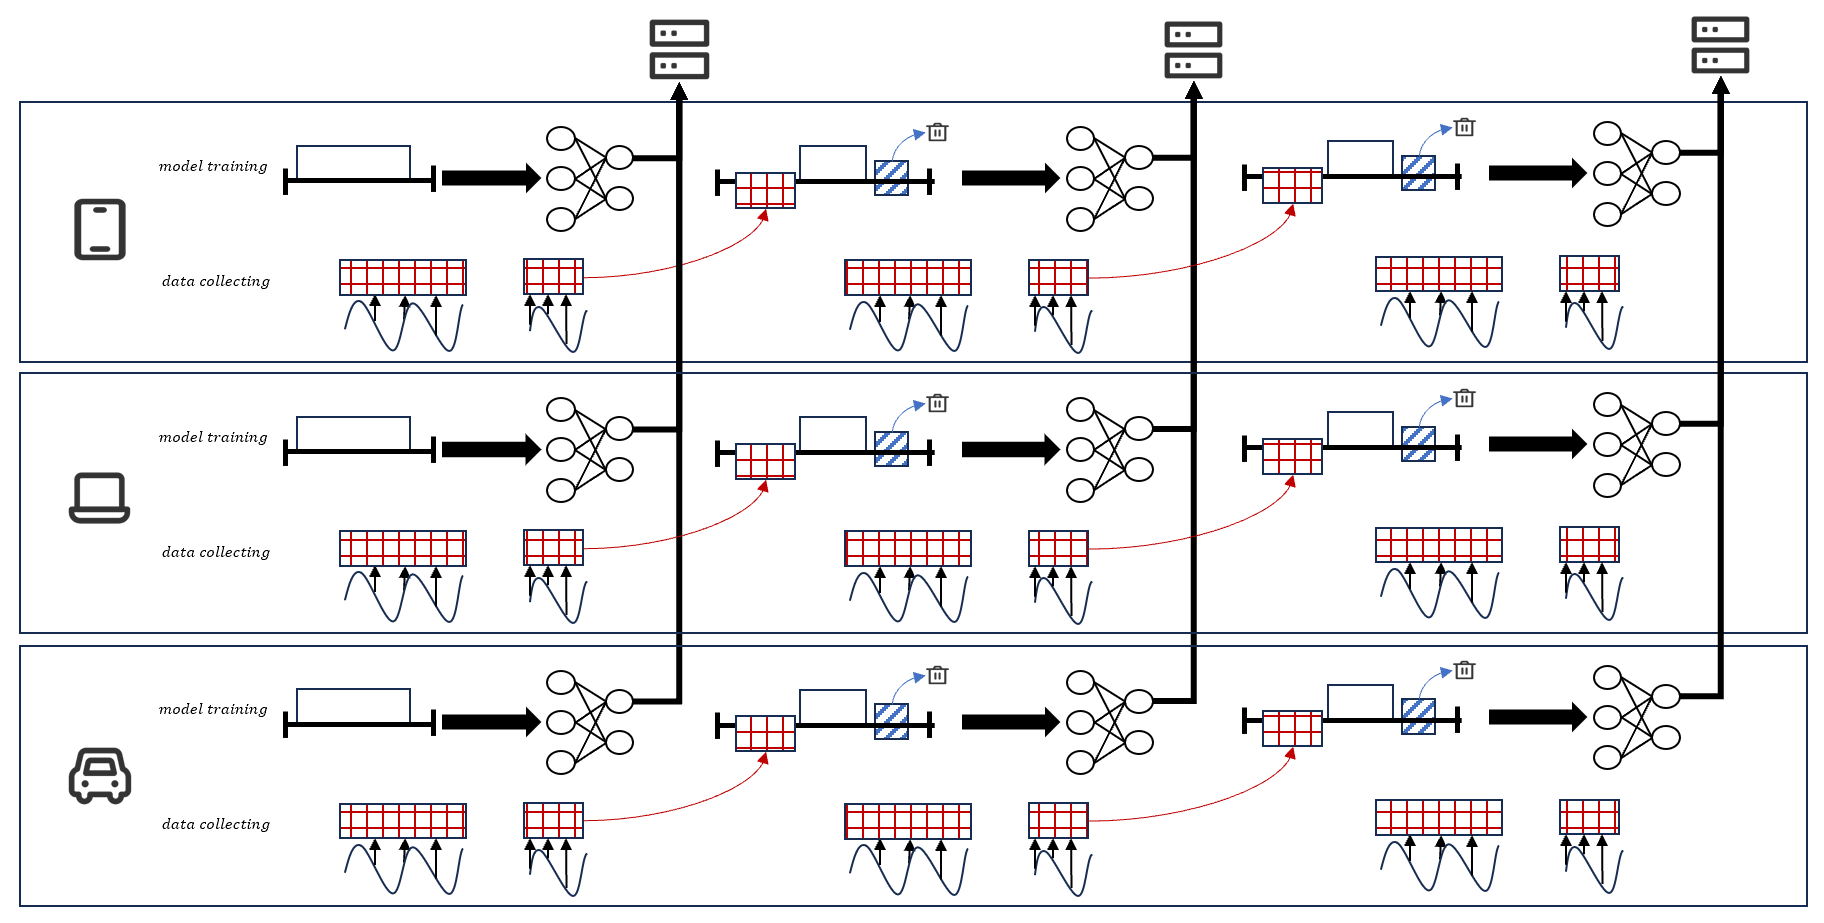
\includegraphics[width=\columnwidth]{figures/figure_21.png}
  \caption{The framework of buffer update scheme. Tilde denotes local data stream. Blank blocks symbolize buffered data, while red blocks and blue blocks symbolize new data to be collected and stale data to be decayed respectively.}
  \label{fig:framework}
\end{figure}
We assume that there is a central server and $N$ clients in the federated learning system and they are arranged to conduct $T$ rounds in the training task. Different from the static local dataset in previous works, each client $k$ has a local data stream $\mathcal{D}_k$ which generates new data points continuously over the time horizon.
In addition, due to the storage limit, each client maintains a buffer to store data points collected from its local data stream $\mathcal{D}_k$ and used for model training.
We denote the stored data points in the buffer of client $k$ at round $t$ as $\mathcal{D}_k(t)$ and $\vert\mathcal{D}_k(t)\vert = D_k(t)$. 
During each round, the buffer of client $k$ can be updated by decaying part of stale data points and collecting new ones from its local data stream, and then used for local model training.
Therefore, the updating scheme of client $k$ at round $t$ can be formulated as
\begin{equation}
  D_k(t+1) = \theta D_k(t) + \Delta_k(t),
  \label{formulation:update}
\end{equation}
where $\theta \in [0,1]$ is the conservation rate of stale data points and it decides how many buffered data can be conserved. 
Besides, $\Delta_k(t)$ is the volume of new data to be collected during round $t$, namely increment. 

Note that considering the uncertainty of data stream, data collection cannot be completed immediately, which means the traditional "collecting-training" paradigm may lead to severe time latency for federated learning task.
To improve the task efficiency, data collection is designed to proceed in parallel with model training in our framework, and the new data collected during present round will be used to update buffer and train model for next round, as depicted in Fig \ref{fig:framework}.

Then, the loss function of client $k$ based on global model $w(t)$ using stored data points $\mathcal{D}_k(t)$ at round $t$ can be represented as 
\begin{equation}
  F_k(w(t), \mathcal{D}_k(t)) = \frac{1}{D_k(t)} \sum_{j=1}^{D_k(t)} f(w(t), x_k^j),
\end{equation}
where $f(w(t), x_k^j)$ is the loss function of each data point $\{x_k^j, y_k^j\} \in \mathcal{D}_k(t)$.
Then client $k$ updates its local model by
\begin{equation}
  w_k(t+1) = w(t) - \eta \nabla F_k(w(t), \mathcal{D}_k(t)),
\end{equation}
where $\eta$ is the learning rate and $\nabla F_k(w(t), \mathcal{D}_k(t))$ is the loss gradient of client $k$ at round $t$. 
Until each client completes its local update and sends $w_k(t+1)$ to the central server, the central server will aggregate them by
\begin{equation}
  w(t+1) = \sum_{k=1}^{N} \frac{D_k(t)}{D(t)} w_k(t+1),
\end{equation}
where $\mathcal{D}(t) = \cup_{k=1}^N \mathcal{D}_k(t)$ and $D(t) = \sum_{k=1}^{N} D_k(t)$.
Subsequently, the central server launches the new global model $w(t+1)$ to each client for the next round's training.
The global loss function at round $t$ can be represented as
\begin{equation}
  F(w(t), \mathcal{D}(t)) = \sum_{k=1}^{N} \frac{D_k(t)}{D(t)} F_k(w(t), \mathcal{D}_k(t)).
\end{equation}
The ultimate goal is to find optimal parameters $w(t), t \in [0, \cdots, T-1]$ to minimize the global loss function in each round $t$, which can be expressed as
\begin{equation}
  \arg \min_{w(t)} F(w(t), \mathcal{D}(t)) = \sum_{k=1}^{N} \frac{D_k(t)}{D(t)} F_k(w_k(t), \mathcal{D}_k(t)).
\end{equation}

\subsection{Convergence Analysis for Federated Learning with Data Stream}
Convergence analysis for model performance is provided in this section.
In practice, it's difficult to measure the model performance of FedStream directly due to data dynamity, data heterogeneity and so on.
Therefore, we provide a convergence upper bound for FedStream, considering the impact of data volume and data staleness on model performance.
Before that, the concept of degree of staleness (DoS) for buffered data is introduced in Definition \ref{definition:1}.
\begin{definition}
  \label{definition:1}
  We denote $S_k(t)$ as the degree of staleness(DoS) for client $k$'s buffered data at round $t$. The recursive definition is provided as 
  \begin{equation}
    \resizebox{\columnwidth}{!}{$
      S_k(t) = 
      \begin{cases}
        \dfrac{\theta D_k(t-1)}{D_k(t)}(S_k(t-1) + 1) + \dfrac{\Delta_k(t-1)}{D_k(t)}, & t > 0; \\
        1, & t = 0,
      \end{cases}
    $}
  \end{equation}
  where $S_k(t)$ is the weighted sum of conserved buffered data's DoS and new data's DoS.
  The conserved buffered data's DoS should be updated by adding to $1$ once stepping into the next time slot, while new data's DoS is set to be $1$.
\end{definition}

\begin{remark}
  $S_k(t)$ increases with conservation rate $\theta$ and decreases with increment $\Delta_k(t)$, which reflects the fact that less conserved buffered data and more fresh data contribute to DoS reduction.
\end{remark}
\begin{remark}
  \label{remark:generalformula}
  The general formula of $S_k(t)$ can be further provided as
  \begin{equation}
    S_k(t) = \sum_{\tau=0}^{t} \frac{\theta^{t-\tau} D_k(\tau)}{D_k(t)}.    
  \end{equation}
\end{remark}
The detailed proof is provided in Appendix \ref{proof:generalformula}.

Next, we introduce some assumptions on local loss function $F_k(w)$ which have been widely used in previous works before the presentation of convergence analysis \cite{wu2023towards} \cite{wei2020federated}.
\begin{assumption}
  Loss function of a particular client $k$ meets the following properties:
  \begin{itemize}
    \item $F_k(w)$ is $\rho$-Lipschitz, i.e., $F_k(w) - F_k(w^{'}) \leq \rho \Vert w - w^{'} \Vert_2$.
    \item $F_k(w)$ is $\beta$-Lipschitz smooth, i.e., $\Vert\nabla F_k(w) - \nabla F_k(w^{'})\Vert \leq \beta \Vert w-w^{'} \Vert_2$.
    \item $F_k(w)$ is $\mu$-strong contex, i.e., $F_k(w)$ satisfies $F_k(w) - F_k(w^*) \leq \frac{1}{2\mu}\Vert\nabla F_k(w)\Vert_2^2$.
    \item The stochastic gradient is unbiased and variance-bounded, that is, $E[\nabla F_k(w(t)|D_k(t))] = \nabla F_k(w(t)|\mathcal{D}_k)$ and $E\Vert\nabla F_k(w(t)|D_k(t)) - \nabla F_k(w(t)|\mathcal{D}_k)\Vert^2 \leq \frac{\psi^2}{D_k(t)}$, where $\psi$ is a constant.
    \item The expected square norm of stochastic gradient is bounded, i.e., $E\Vert \nabla F_k(w(t)|D_k(t))\Vert^2 \leq G_k^2 + S_k(t)\sigma^2$, where $\sigma$ is a constant to measure the time sensitivity of the server's tasks.
  \end{itemize}
  \label{assumption}
\end{assumption}
\begin{theorem}
  \label{theorem:upperbound}
  Under Assumption \ref{assumption}, with $\eta \leq \frac{1}{2\beta}$, the convergence upper bound after $T$ rounds can be formulated as
    \begin{align}
      & E[F(w(T)|D(T)) - F(w^*)] \notag \\
      \leq & \underbrace{\vphantom{\sum_{min}^{max}\frac{1}{2}} \kappa_1^{T} E[F(w(0)|D(0))-F(w^*)]}_{(1)} \notag \\
      & + \sum_{t=0}^{T-1} \kappa_1^{T-1-t} \left[\underbrace{\vphantom{\sum_{min}^{max}\frac{1}{2}} \kappa_2 \frac{N\psi^2}{D(t)}}_{(2)} + \underbrace{\vphantom{\sum_{min}^{max}\frac{1}{2}} \kappa_3 \sum_{k=1}^{N} \frac{D_k(t)}{D(t)} S_k(t) \sigma^2}_{(3)} + \underbrace{\vphantom{\sum_{min}^{max}\frac{1}{2}} \Omega_{t}}_{(4)}\right]. \notag \\ 
    \end{align}
  where $\Omega_t = F(w(t+1)|D(t+1)) - F(w(t+1)|D(t))$.
  In addition, $\kappa_1 = 1 + 4\mu\beta\eta^2 - 2\mu\eta$, $\kappa_2 = 2\beta\eta^2$, $\kappa_3 = \beta\eta^2$. 
\end{theorem}

The detailed proof is provided in Appendix \ref{proof:upperbound}.
\begin{remark}
  In Theorem \ref{theorem:upperbound}, the second term and the third term measures the influence of data volume and staleness on model performance respectively. Intuitively, the more and fresher buffered data are, the better global model performs.
  But in FedStream, staleness reduction partly depends on decaying stale data more intensively, which may lead to decrease of data volume, too. Thus, there exists a trade-off between data volume and staleness.
  In addition, the greater $\sigma$ is, the more the third term weighs in the entire upper bound, which reflects the fact that highly time-sensitive tasks are affected more heavily by data staleness. 
\end{remark}
\begin{remark}
  In Theorem \ref{theorem:upperbound}, the fourth term of $\Omega_t$ captures the expected difference of global loss function based on the same global model $w(t)$ between buffered data at present round $\mathcal{D}(t)$ and at previous round $\mathcal{D}(t-1)$.
  Note that $\Omega_t$ is time-varying and it measures the influence of data dynamity has on model performance, and describes the generalization of global model towards new data points. 
  The more fluctuating data dynamity is, the larger the convergence bound is and the worse the global model performs. 
\end{remark}

\section{System Model}
\label{section:system model}
In this section, we design an incentive mechanism for FedStream.
First, we construct optimization problems for both server and clients in \ref{section:cost function} and \ref{section:utility function}.
Then we model them as a two-stage Stackelberg game with dynamic constraint of local update.
\begin{figure}[ht]
  \centering
  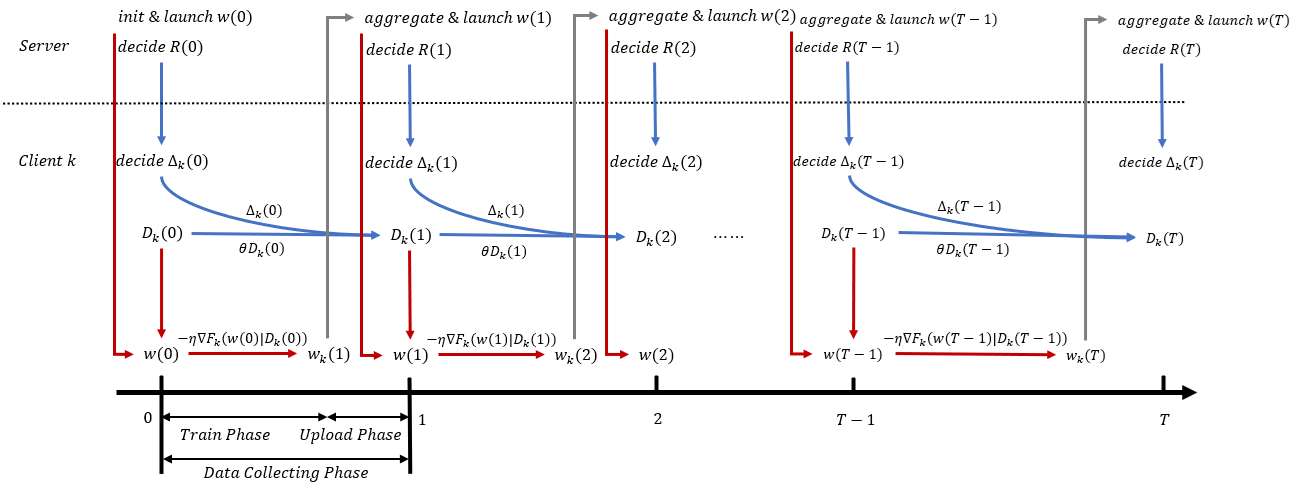
\includegraphics[width=\columnwidth]{figures/figure_17.png}
  \caption{The overview of incentive mechanism. Red lines denote model parameter flow while blue lines symbolize decision and data flow.}
  \label{fig:overview}
\end{figure}

\subsection{Cost Function of Server}
\label{section:cost function}
The cost of the server comprises two parts: accuracy loss of model and payment to clients. 
In reality, it's extremely hard to obtain accurate form of model accuracy loss directly. Yet we can approximate it with the convergence upper bound provided in Theorem \ref{theorem:upperbound}.
Note that $(1)$ and $(5)$ in Theorem \ref{theorem:upperbound} can't be controlled by the server, thus we extract the valid part of $(2)$ and $(3)$ to the cost function.
In addition, total payment during the training period offered to clients can be represented as $TR$.
Then, cost function of the server can be constructed as
\begin{align}
  \label{formulation:cost}
  U(\mathcal{D}, R, \theta) & = \sum_{t=0}^{T-1} \gamma R + (1-\gamma)\kappa_1^{T-1-t} \times \\
  & \left[\left(\kappa_2 \frac{N\psi^2}{D(t)} + \kappa_3 \sum_{k=1}^{N} \frac{D_k(t)}{D(t)} S_k(t) \sigma^2 \right) \right], \notag
\end{align}
where $\gamma \in [0, 1]$ is a factor to balance model performance and cost payment. When $\gamma$ trends to $1$, the server pays more attention to model performance, and vice versa.

(\ref{formulation:cost}) is dominated by payment $R$, conservation rate $\theta$ and total data volume $\boldsymbol{D}$.
The server controls two variables: $R$ intented to encourage clients to collect new data, and $\theta$ intented to order clients to abandon parts of buffered data.
It targets to minimize cost function in (\ref{formulation:cost}). Thus the optimality problem on the server side can be constructed as 
\begin{equation}
  \label{formulation:mincost}
  \min_{R,\theta}  U(\boldsymbol{D}, R, \theta), 
\end{equation}
In (\ref{formulation:mincost}), greater reward incurs more fresh data for model training but increases monetary payment, while smaller conservation rate forces to abandon more stale data but decreases data volume at the same time. This is non-trivial and the server needs to minimize cost by elaborately determining the strategy of $(R, \theta)$.


\subsection{Utility Function of Clients}
\label{section:utility function}
For a client who participates into the federated learning task, it needs to spend various types of resource for data sampling and model training.
Here, we use $\alpha_k \Delta_k(t)^2$ and $\beta_k D_k(t)^2$ to depict the expenditure for data collecting and training, respectively, where $\alpha_k$ is unit cost for data collecting and $\beta_k$ is the counterpart for model training.
It should be noted that we choose the quadratic form of $\Delta_k(t)^2$ and $D_k(t)^2$ to reflect the fact that a client's sampling and training expenditure should convexly increase with its increment and scale, respectively \cite{wang2019dynamic}.
Therefore, the cost can be expressed as
\begin{equation}
  C_k(t) = \alpha_k \Delta_k(t)^2 + \beta_k D_k(t)^2.
\end{equation}

Meanwhile, a client can obtain some reward.
In FedStream, the reward a particular client can secure depends on its buffered data compared with other participating clients, which can be formulated as
\begin{equation}
  P_k(t) = \frac{D_k(t)}{\sum_{i=1}^{N}D_i(t)}R.
\end{equation}
Then, utility function of a particular client $k$ is constructed as the sum of balance over the time horizon:
\begin{equation}
  \label{formulation:maxutility}
  U_k(\boldsymbol{D_k}, \boldsymbol{D_{-k}}, R, \theta) = \sum_{t=0}^{T-1} \left(P_k(t) - C_k(t)\right),
\end{equation}

(\ref{formulation:maxutility}) is dominated by its own buffered data volume vector $\boldsymbol{D_k}$, others buffered data volume vector $\boldsymbol{D_{-k}}$, the server's payment $R$ and conservation rate $\theta$.
Client $k$ only controls its own increment $\Delta_k(t)$, a time-varying variable to influence its data volume indirectly.
It aims to maximize utility function in (\ref{formulation:maxutility}) under the constraint in (\ref{formulation:update}).
Hence, the optimization problem for a particular client $k$ can be constructed as
\begin{equation}
  \begin{aligned}
    \max_{\boldsymbol{\Delta_k}=[\Delta_k(t)] \atop t \in [0,\cdots,T-1]} & U_k(\boldsymbol{D_k}, \boldsymbol{D_{-k}}, R, \theta), \\
    \text{s.t.} & D_k(t + 1) = \theta D_k(t) + \Delta_k(t),
  \end{aligned}  
\end{equation}

\subsection{Stackelberg Game Formulation}
Based on the discussions in \ref{section:cost function} and \ref{section:utility function}, we use a two-stage Stackelberg Game to model the interaction between the server and clients as
\begin{equation}
  \begin{aligned}
    \mathrm{Stage\ \uppercase\expandafter{\romannumeral1}:} & 
    \min_{R, \theta}  U(\boldsymbol{D}, R, \theta), \\
    \mathrm{Stage\ \uppercase\expandafter{\romannumeral2}:} &
    \max_{\boldsymbol{\Delta_k}=[\Delta_k(t)] \atop t \in [0,\cdots,T-1]} U_k(\boldsymbol{D_k}, \boldsymbol{D_{-k}}, R, \theta), \\
    & \text{s.t.} D_k(t + 1) = \theta D_k(t) + \Delta_k(t),
  \end{aligned}  
\end{equation}
where the server acts as a leader and clients are regarded as followers.
The overview of incentive mechanism is depicted in Figure \ref{fig:overview}. Before each round, the server launches its optimal strategy of $(R, \theta)$ to clients in Stage \uppercase\expandafter{\romannumeral1}.
Then in Stage \uppercase\expandafter{\romannumeral2}, according to $(R, \theta)$ announced by the server, each client $k \in \mathcal{N}$ decides its optimal strategy of $\Delta_k(t)$.
As a result, the equilibrium of this game guarantees mutual optimality between the server and clients.

\section{Methodology}
In this section, we derive the equilibrium of the Stackelberg game in last section.
By means of backward reduction, we provide the optimal strategy for clients and the server progressively.

\subsection{Introduction of Mean-Field Term}
\label{section:mean-field term}
For a particular client $k$, it needs to learn about the server's strategy $(R, \theta)$ and the total buffered data volume $\sum_{i=1}^N D_i(t)$ before deriving the optimal strategy at round $t$.
However, in many real-world scenarios, the term of $\sum_{i=1}^{N}$ keeps unknown to client $k$ due to information isolation among clients.
To tackle this problem, we introduce a mean-field term $\phi(t)=\sum_{i=1}^{N} D_i(t)$. From the perspective of mathematics, $\phi(t)$ is a given function and it can be considered as a known term.
We replace $\sum_{i=1}^{N} D_i(t)$ in (\ref{formulation:maxutility}) with it, and the optimization problem of client $k$ can be reformulated as
\begin{align}
  \label{formulation:reformulated}
  \max_{\boldsymbol{\Delta_k}=[\Delta_k(t)] \atop t \in [0,\cdots,T-1]} & \sum_{t=0}^{T-1} \left(\frac{D_k(t)}{\phi(t)}R - \alpha_k\Delta_k(t)^2 - \beta_kD_k(t)^2\right), \notag \\
  \text{s.t.} & D_k(t+1) = \theta D_k(t) + \Delta_k(t).
\end{align}


Besides, the estimation of $\phi(t)$ is arranged in Section \ref{section:estimation}.


\subsection{Optimal Strategy of Clients in Stage \uppercase\expandafter{\romannumeral2}}
In stage \uppercase\expandafter{\romannumeral2}, provided the strategy $(R, \theta)$ launched by the server, we derive the optimal strategy of $\Delta_k(t)$ for client $k$ at round $t$.
However, client $k$ faces a long-term optimization problem with dynamic constraint of update strategy.
Thus, we adopt Hamilton equation to solve the problem in stage \uppercase\expandafter{\romannumeral2}. Then we have the following proposition.
\begin{proposition}
  \label{proposition:clientoptimalstrategy}
  For any client $k$ at arbitray round $t$, the optimal increment $\Delta_k(t)$ is
  \begin{equation}
    \resizebox{\columnwidth}{!}{$
      \Delta_k(t) = 
      \begin{cases}
        \max\left\{\frac{1}{2 \alpha_k} \sum_{\tau = t + 1}^{T - 1} \theta^{\tau - t - 1} \left(\frac{R}{\phi(\tau)} - 2\beta_k D_k(\tau)\right), 0\right\}, & t \in [0, T-2]; \\
        \displaystyle 0, & t = T-1.
      \end{cases}    
    $}
  \label{formulation:delta}
  \end{equation}
  Furthermore, the optimal buffer size $D_k(t)$ is
  \begin{equation}
    \resizebox{\columnwidth}{!}{$
      D_k(t) = 
      \begin{cases}
        \displaystyle D_0, & t = 0; \\
        \theta^{t} D_k(0) + \sum_{\tau = 0}^{t-1} \theta^{t-1-\tau} \Delta_k(\tau), & t \in [1, T-1].
      \end{cases}
    $}
  \label{formulation:datasize}
  \end{equation}
\end{proposition}
The detailed proof is provided in Appendix \ref{proof:clientoptimalstrategy}.
\begin{remark}
  (\ref{formulation:delta}) reveals that provided $R, \theta$ and $\phi(t)$, $\Delta_k(t)$ is affected by the subsequent buffered data volume of $D_k(\tau), \tau \in [t+1, \cdots, T]$, which in turn affects $\Delta_k(t)$ according to (\ref{formulation:datasize}).
  Therefore, a close loop exists between $\boldsymbol{\Delta}_k$ and $\boldsymbol{D}_k$, where greater $\boldsymbol{\Delta}_k$ leads to greater $\boldsymbol{D}_k$, which in turn inhibits $\boldsymbol{\Delta}_k$.
\end{remark}
\begin{remark}
  A stationary state exists against increment $\Delta_k(t)$ in an infinite time horizon.
  The detailed proof is provided in Appendix \ref{proof:stationary state}.
  \label{remark:stationary state}
\end{remark}


\subsection{Optimal Strategy of Server in Stage \uppercase\expandafter{\romannumeral1}}
In stage \uppercase\expandafter{\romannumeral2}, provided all clients' optimal strategy of $\boldsymbol{\Delta}_k, k \in [N]$, we derive the optimal strategy of $(R^*, \theta^*)$ for the server.
But the server faces a two-variable optimization problem in complicated form, which makes it hard to derive a close-form solution of $(R^*, \theta^*)$ for the server.
Thus, we explore the approximately optimal strategy for the server by adopting searching algorithms.

\subsection{Estimation of Mean-Field Term}
\label{section:estimation}
Ultimately, we try to estimate $\phi(t), t\in[0,\cdots,T-1]$, the mean-field term introduced in section \ref{section:mean-field term} by means of fixed point algorithm.
According to (\ref{formulation:datasize}), $D_k(t)$ is a function of $\Delta_k(\tau), \tau \in [0,\cdots,t-1]$. By inserting (\ref{formulation:delta}) into (\ref{formulation:datasize}), $D_k(t)$ is actually a function of $\phi(t)$ and $D_k(t), t \in [0, \cdots, T-1]$.
We define this function as
\begin{align}
  D_k(t) = \Psi_{k,t}( & \phi(0), \phi(1), \cdots, \phi(T-1), \\
                       & D_k(0), D_k(1), \cdots, D_k(T-1)).
\end{align}
Furthermore, $\phi(t)$ is a function of $D_k(t), k \in [1, \cdots, N]$ at round $t$, so it can be derived that $D_k(t)$ is a function of $D_k(t), k \in [1, \cdots, N], t \in [0, \cdots, T-1]$. That is
\begin{align}
  \label{formulation:matrix}
  D_k(t) = \Psi_{k,t} & (D_1(0), D_1(1), \cdots, D_1(T-1), \notag \\
                      & D_2(0), D_2(1), \cdots, D_2(T-1), \notag \\
                      & \cdots, \notag \\
                      & D_N(0), D_N(1), \cdots, D_N(T-1)).
\end{align}
For ease of reading, we denote the parameter matrix in (\ref{formulation:matrix}) as $A$. Then we have $D_k(t) = \Psi_{k,t}(A)$.
To summarize buffered data volume $D_k(t)$ over the time horizon $t \in [0, \cdots, T-1]$ and $k \in [1, \cdots, N]$, we have the following vector function as
\begin{align}
  A = & \Psi(A) \notag \\
    = & (\Psi_{1, 0}(A), \Psi_{1, 1}(A), \cdots, \Psi_{1, T-1}(A) \notag \\
      & \Psi_{2, 0}(A), \Psi_{2, 1}(A), \cdots, \Psi_{2, T-1}(A) \notag \\
      & \cdots, \notag \\
      & \Psi_{K, 0}(A), \Psi_{K, 1}(A), \cdots, \Psi_{K, T-1}(A)),
\end{align}
which is a mapping from $A$ to $A$.
Then we have the following proposition.
\begin{proposition}
  \label{proposition:fixed point}
  $\Psi$ has a fixed point.
\end{proposition}
The detailed proof is provided in Appendix \ref{proof:fixed_point}
Based on Proposition \ref{proposition:fixed point}, we can adopt fixed point algorithm to estimate $\phi(t)$ precisely.

\subsection{Description of Algorithm}

 \begin{algorithm}[tb]
    \caption{\texttt{Client-Strategy}}
    \begin{algorithmic}[1]
        \STATE{\bfseries Input:} $\phi, R, \theta$.
        \STATE{\bfseries Output:} $\Delta_k(t), D_k(t), t \in [0, \cdots, T -1], k \in [1, \cdots, N]$.
        \STATE{\bfseries Initialize:} $D_k^0(t), t \in [0, \cdots, T - 1], k \in [1, \cdots, N], j=0, \epsilon$.
        \REPEAT
            \FOR{$t = 0$ {\bfseries to} $T - 1$}
                \FOR{$k = 1$ {\bfseries to} $N$}
                    \STATE Calculate $\Delta_k^j(t)$ using $\phi, R, \theta$ and $D_k^j(t)$ according to (17).
                    \STATE Calculate $D_k^j(t)$ using $\Delta_k^j(t)$ according to (18).
                \ENDFOR
            \ENDFOR
            \STATE $j \gets j + 1.$
        \UNTIL{$D_k^{j+1}(t) - D_k^j(t) \leq \epsilon, k \in [1, \cdots, K], t \in [0, \cdots, T - 1]$}.
    \end{algorithmic}
 \end{algorithm}

 \begin{algorithm}[tb]
    \caption{\texttt{Server-Strategy}}
    \begin{algorithmic}[1]
        \STATE {\bfseries Input:} $\phi$.
        \STATE {\bfseries Output:} $R, \theta$.
        \STATE {\bfseries def} Func($R, \theta$):
        \STATE \hspace{1em} $D_k(t) \gets \texttt{Client-Strategy}(\phi, R, \theta)$.
        \STATE \hspace{1em} Calculate {\it res} using $D_k(t)$ according to (16).
        \STATE \hspace{1em} {\bfseries return} \it{res}.
        \STATE $R^*, \theta^* \gets$ \texttt{PSO}(\texttt{Func}).
        \STATE {\bfseries return} $R^*, \theta^*$.
    \end{algorithmic}
\end{algorithm}

\begin{algorithm}[tb]
    \caption{\texttt{Estimate-MFT}}
    \begin{algorithmic}[1]
        \STATE{\bfseries Input:} None.
        \STATE{\bfseries Output:} $\phi_k(t), k \in [1, \cdots, N], t \in [0, \cdots, T - 1]$.
        \STATE{\bfseries Initialize:} $\phi_k^0(t), k \in [1, \cdots, N], t \in [0, \cdots, T - 1], j=0, \epsilon$.
        \REPEAT
            \STATE $R, \theta \gets \texttt{Server-Strategy}(\phi)$.
            \STATE $D_k(t) \gets \texttt{Client-Strategy}(\phi, R, \theta)$.
            \FOR{$t = 0$ {\bfseries to} $T - 1$}
                \STATE Calculate $\phi_k^j(t)$ using $D_k^j(t)$ according to (20).
            \ENDFOR
            \STATE $j \gets j + 1.$
        \UNTIL{$D_k^{j+1}(t) - D_k^j(t) \leq \epsilon, k \in [1, \cdots, K], t \in [0, \cdots, T - 1]$}.
    \end{algorithmic}
 \end{algorithm}

 \begin{algorithm}
    \caption{\texttt{Main Procedure}}
    \begin{algorithmic}[1]
        \STATE{\bfseries Input: } $T, N$.
        \STATE{\bfseries Output: } $w(T)$.
        \STATE{\bfseries Initialize: } $w(0)$.
        \STATE $\phi \gets \texttt{Estimate-MFT}()$.
        \STATE $R, \theta \gets \texttt{Server-Strategy}(\phi)$.
        \STATE $\Delta, D \gets \texttt{Client-Strategy}(\phi, R, \theta)$.
        \FOR{$t = 0$ {\bfseries to} $T - 1$}
            \STATE Server distributes global model $w(t)$ to clients.
            \FOR{each client $k$  {\bfseries in parallel}} 
                \STATE Abandon $\theta D_k(t-1)$ data points randomly from buffer: $\widetilde{D}_k(t) = D_k(t-1) - \theta D_k(t-1)$.
                \STATE Collect $\Delta_k(t-1)$ data points from local data stream: $D_k(t) = \widetilde{D}_k(t) + \Delta_k(t-1)$.
                \STATE Execute local update with global model $w(t)$: $w_k(t+1) = w(t) - \eta \nabla F_k(w(t)|D_k(t))$. 
                \STATE Upload local model $w_k(t+1)$ back to the server.
            \ENDFOR
            \STATE Server aggregates local model $w_i(t+1), i \in [N]$: $w(t+1) = \sum_{i=1}^{N} \frac{D_i(t+1)}{\sum_{i=1}^{N}D_i(t+1)} w_i(t+1)$.
        \ENDFOR
        \STATE {\bfseries return} $w(T)$.
    \end{algorithmic}
 \end{algorithm}

\section{Experiment}
In this section, we evaluate the performance of proposed FedStream by numerical experiments.
\subsection{Experimental Setup}
\textbf{Datasets and Models: }
We conduct our experiments in two widely used real datasets: MNIST and FMNIST.
The MNIST dataset contains 60,000 training samples and 10,000 test samples for handwrittern digit recognization.
The FMNIST dataset comprises 50,000 training samples and 10,000 test samples for fashion item recognization.
To simulate the impact of DoS in practical training, we mislabel parts of local buffer data of each client before each time slot, which is similar to the method adopted in \cite{xu2024age}. 
The proportion of mislabeling depends on time sensitivity coefficient $\sigma$. If we set a greater $\sigma$, which corresponds to a higher time-sensitive FL task, then the proportion of mislabeling will rise and vice versa.
Besides, to simulate the setting of local data stream $\mathcal{D}$, we assign the dataset into all clients beforehand in a IID method. During the task, each client will sample new data from local dataset to its buffer according to the optimal strategy.
Lastly, we use CNN as the training model in our experiments, which is made up of two sets of convolution layers and max pooling layers, and then two fully-connected layers and a RELU layer.

\textbf{Hyperparameters Settings: }
We consider a federated learning setting with the number of rounds $T = 20$. In each round, there are 10 clients participating in the training.
For a particular client $k$, it holds an initial buffer data with volume $D_k(0) = 700$ by default. During training, the unit price of data collection and training is set to be $\alpha_k \sim U(10^{-4}, 10^{-3})$ and $\beta_k \sim U(5^{-6}, 5^{-5})$ respectively. Each client conducts one local update at a round with learning rate $\eta=10^{-2}$.
In addition, the server's cost balance factor is $\gamma = 10^{-4}$, with time sensitivity coefficient of $\sigma = 1$ and strategy space of $\theta \in [0, 1]$, $R \in [0, 100]$.

As for the hyperparameters of $\kappa_2, \kappa_3$ and $\kappa_4$, we take the similar method adopted in \cite{wang2019adaptive} and \cite{huang2024collaboration}, both of which estimate these values with a simple FL training procedure.
By conducting the simple procedure, we obtain $\kappa_2 = 1$ and  $\kappa_3 = \kappa_4 = 10^{-2}$.
% 补变旧效果
% 补仿照超参数设置
\subsection{Experimental Results}
\textbf{Iteration of Mean-Field Term: }
\begin{figure}
	\begin{minipage}{0.49\linewidth}
		\vspace{3pt}
        %这个图片路径替换成你的图片路径即可使用
		\centerline{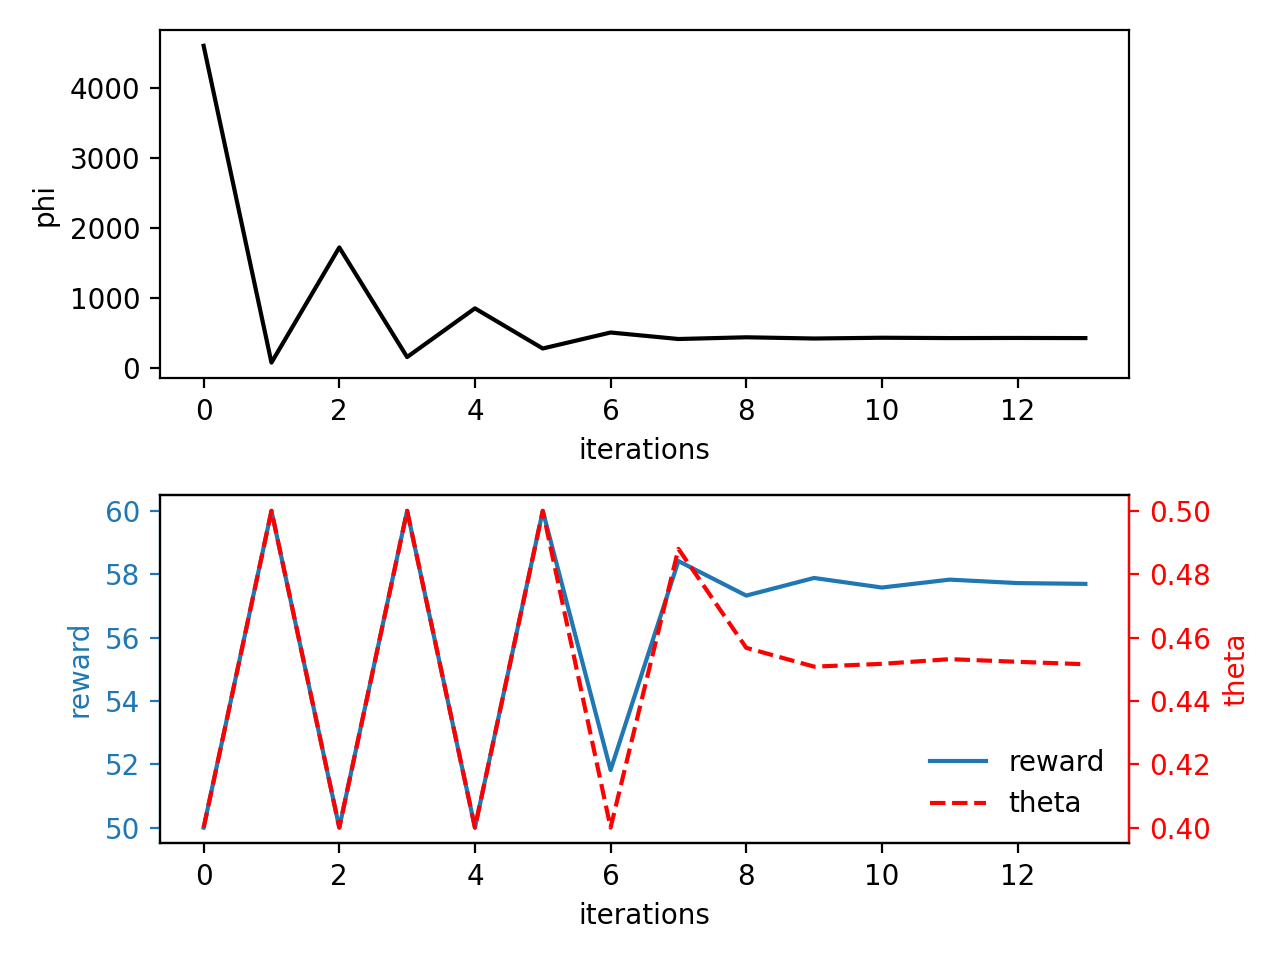
\includegraphics[width=\textwidth]{figures/figure_38.png}}
          % 加入对这列的图片说明
		\centerline{$N=3, T=5$}
	\end{minipage}
	\begin{minipage}{0.49\linewidth}
		\vspace{3pt}
		\centerline{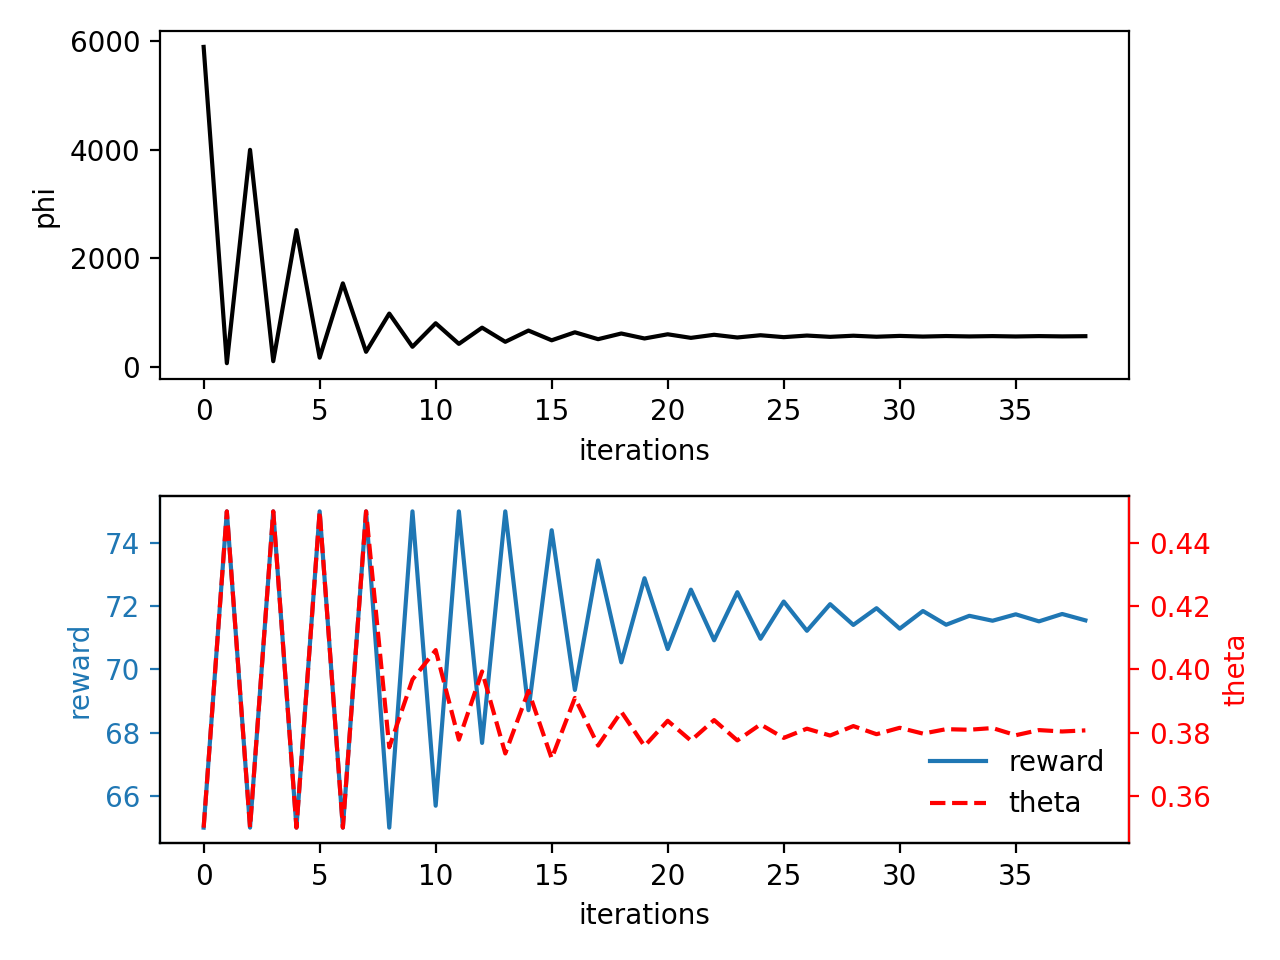
\includegraphics[width=\textwidth]{figures/figure_39.png}}
		\centerline{$N=5, T=10$}
	\end{minipage}
	\caption{The iteration of $\phi$, $R, \theta$ and $\Delta$}
\end{figure}

\textbf{Effect of Client's Strategy on its Utility: }
In this paragraph, we analyse the effect of increment strategy $\Delta_k(t)$ on clients' utility and the results are plotted in Figure \ref{fig:clients}.
For comparison, we implement two auxiliary strategies: zero strategy and random strategy. For a particular client $k$, zero strategy means it doesn't collect any new data through the training procedure, while random strategy refers that it collects new data randomly in each time slot. Note that in order to keep comparison meaningful, the total amount of new data collected over the time horizon under random strategy is set to be roughly consistent with that under optimal strategy.
We can find optimal strategy helps client $k$ secure the highest utility comparied with other two strategies.
Provided clients are selfish, this indicates that each of them will follow the optimal strategy, thereby the mutually best response strategies are reached simultaneously, which meets the requirement the Nash equilibrium solution of Stage \uppercase\expandafter{\romannumeral2}.
In addition, we can find under the same increment strategy, the client's utility $U_k$ decreases with number of clients $N$. The underlying reason is that clients expansion may intensify the competition for a fixed reward among them, thereby leads to reward reduction and utility reduction.
\begin{figure}
	\begin{minipage}{0.49\linewidth}
		\centerline{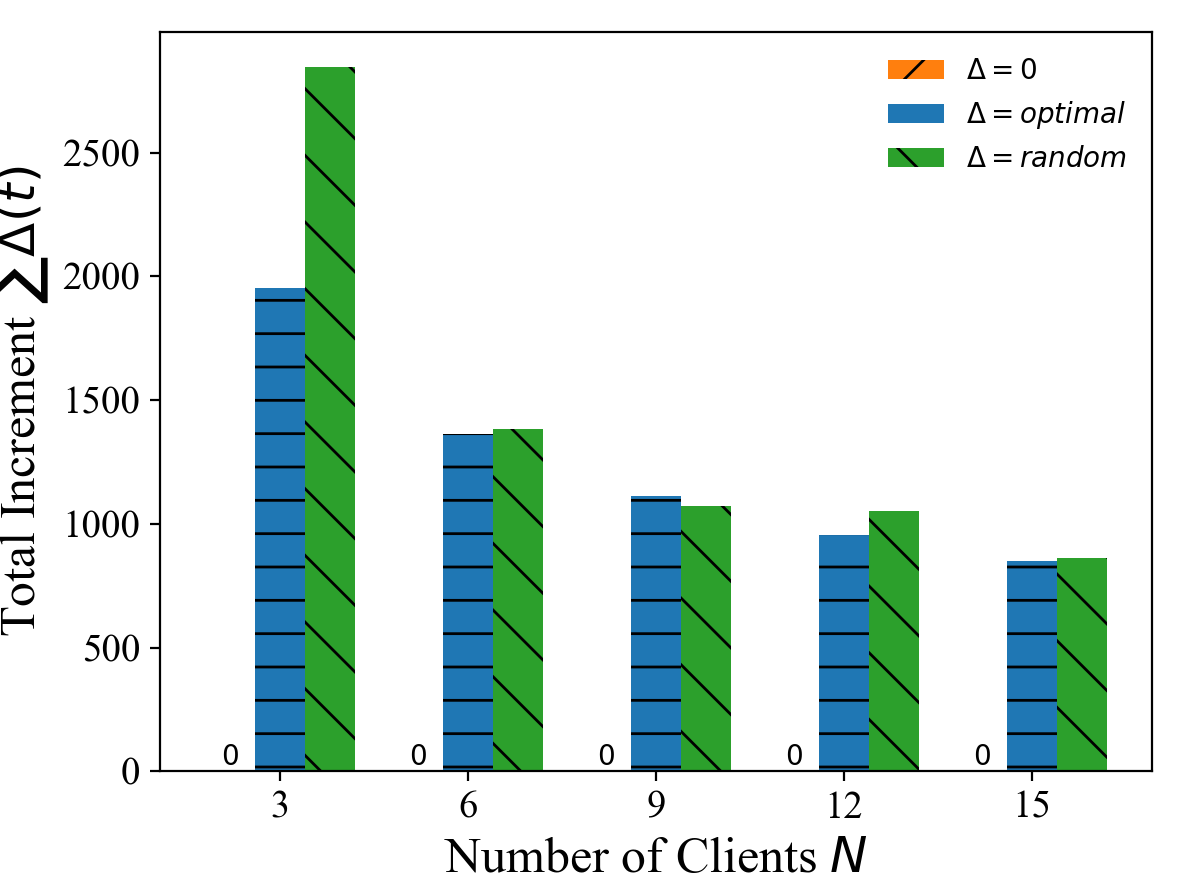
\includegraphics[width=\textwidth]{figures/figure_60_A.png}}
	\end{minipage}
	\begin{minipage}{0.49\linewidth}
		\centerline{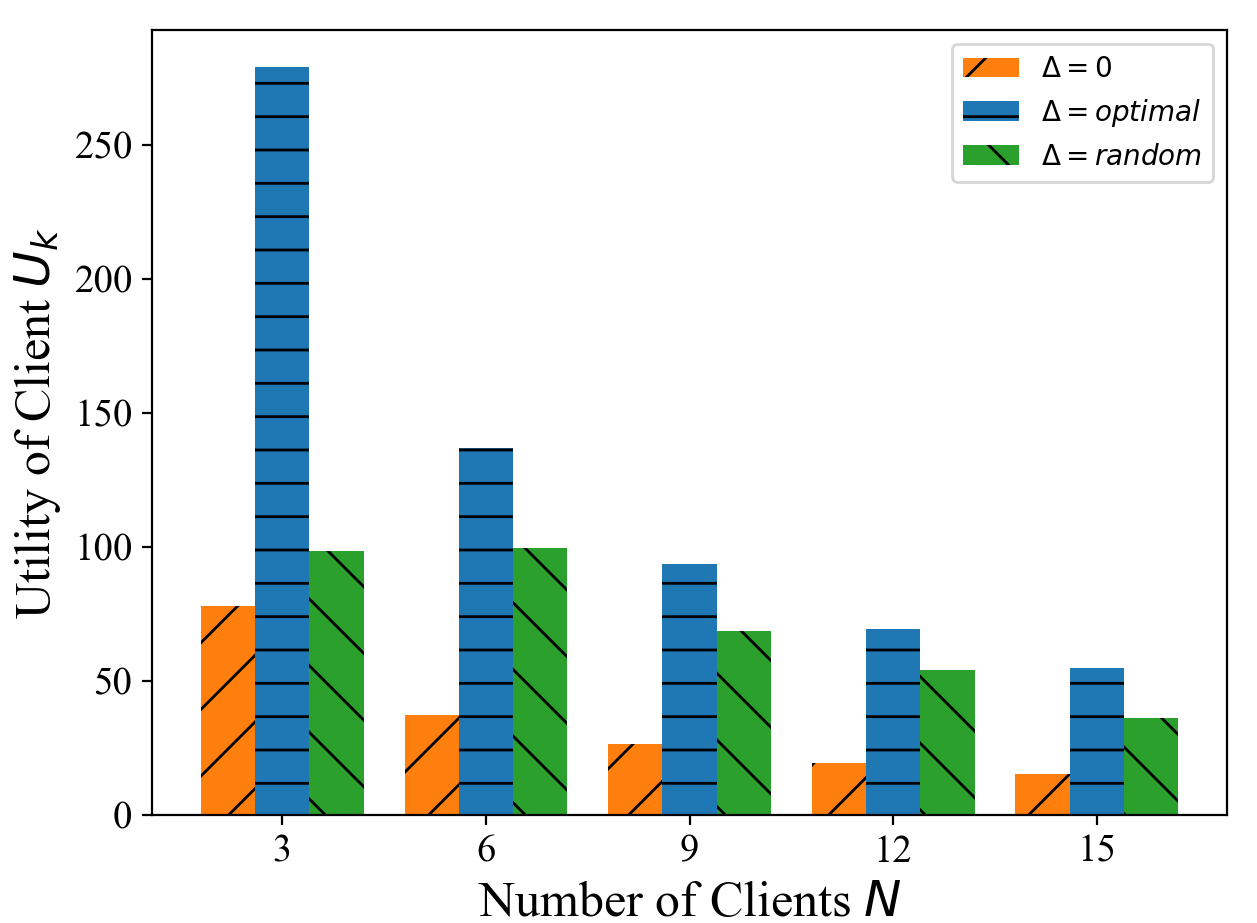
\includegraphics[width=\textwidth]{figures/figure_60_B.png}}
	\end{minipage}
	\caption{Comparative analysis of total increment $\sum_{t=0}^{T-1} \Delta_k(t)$ (\textbf{left}) and utility function $U_k$ (\textbf{right}) against a particular client $k$ versus number of clients $N$ across three increment strategies, including $\Delta_k(t) = 0$, optimal and random.}
    \label{fig:clients}
\end{figure}

\textbf{Effect of Server's Strategy on Average Buffer Data: }
In this paragraph, we study the effect of server's strategy of both reward $R$ and conservation rate $\theta$ on average buffer data from three terms: average increment $\Delta(t)$, average data size $D(t)$ and average data staleness $S(t)$. The results are depicted in Figure \ref{fig:server_increment}, \ref{fig:server_datasize} and \ref{fig:server_staleness} respectively.
Specially, we fix the reward $R_0=61.62$ and consider four types of strategies: $\pi_1=(R_0, 0.1)$, $\pi_2=(R_0, 0.5)$, $\pi_3=(R_0, 0.7)$, $\pi_4=(R_0, 0.9)$. Besides, we also fix $\theta_0=0.3$ and consider another four strategies: $\pi_5=(30, \theta_0)$, $\pi_6=(60, \theta_0)$, $\pi_7=(100, \theta_0)$, $\pi_8=(140, \theta_0)$.

According to Figure \ref{fig:server_increment}, provided a fixed $R$, $\Delta(t)$ decreases with $\theta$. The underlying realistic meaning is that the more valuable previous data are, the greater $\theta$ is set by central server to conserve previous data, thereby the less necessarily central server recruits new data.
In contrast, given a fixed $\theta$, $\Delta(t)$ increases with $R$. That's because a greater reward can effectively stimulate clients to collect more new data for training.
In addition, we notice that $\Delta(t)$ steps into a stationary state after several communication rounds no matter the strategy $\pi$, and then converges to $0$ before the end of training.
The observation of stationary state is substantiated by remark \ref{remark:stationary state}, wherein it is illustrated that a stationary state exists in an dynamic circumstance where clients adopts updated method based on (\ref{formulation:update}).
And the convergence trend to $0$ is also in line with the boundary condition proposed in (\ref{formulation:delta}).

For data volume $D(t)$, as shown in Figure \ref{fig:server_datasize}, the volume of buffer data $D(t)$ increases with both $\theta$ and $R$ since greater $\theta$ means to conserve more previous data and greater $R$ means to collect more new data from local data stream.
Besides, the stationary state of $D(t)$ keeps pace with that of $\Delta(t)$ according to (\ref{formulation:datasize}).

The observation against staleness $S(t)$ is not the same as that against volume. In Figure \ref{fig:server_staleness}, we can find as $\theta$ grows, $S(t)$ soars to an unacceptable level because of rapid accumulation of deteriorated previous data. Yet it seldom effected by the change of $R$. Thus, the observation demonstrates that $S(t)$ is dominated by $\theta$ rather than $R$. It's not trivial to strike the balance between data volume and staleness by adjusting $\theta$ for a better model performance. 

\begin{figure}
	\begin{minipage}{0.49\linewidth}
		\centerline{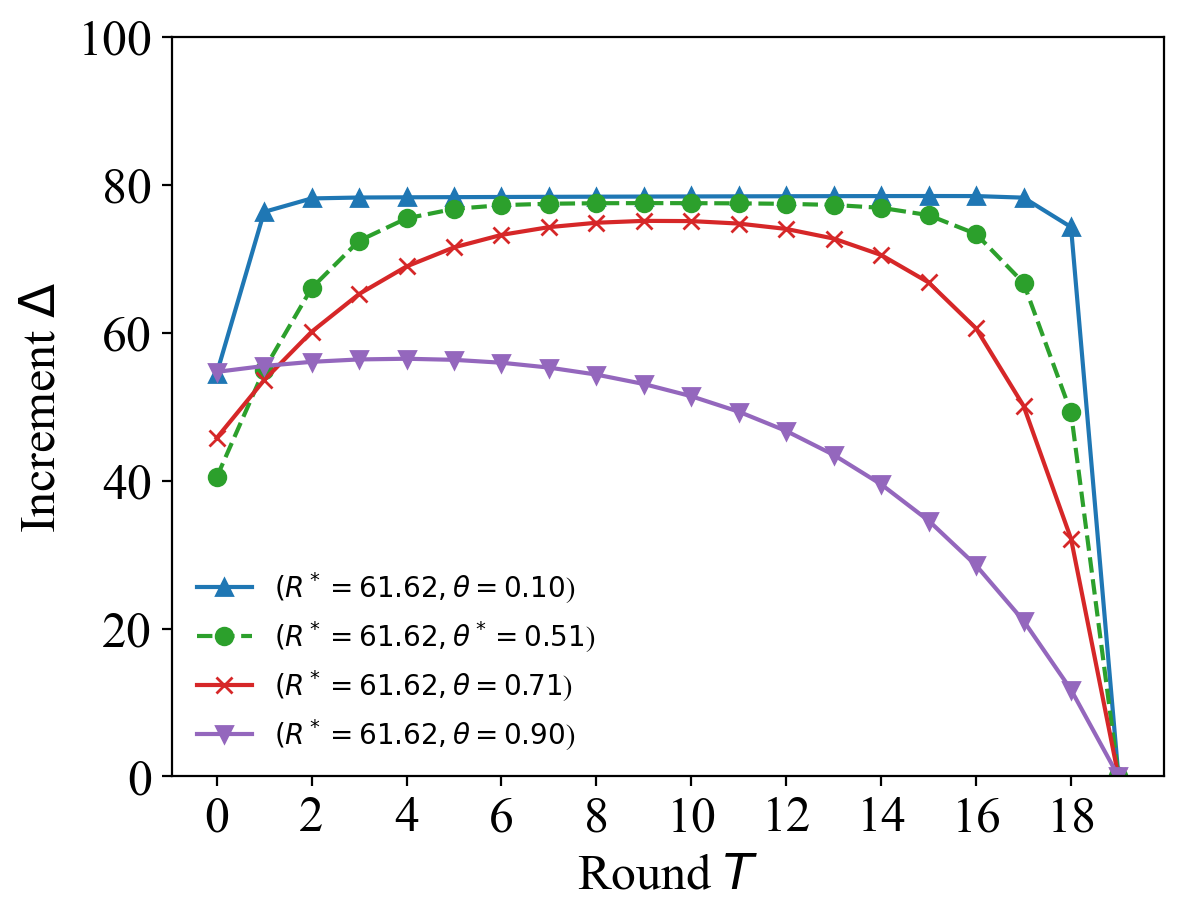
\includegraphics[width=\textwidth]{figures/figure_62_B.png}}
	\end{minipage}
	\begin{minipage}{0.49\linewidth}
		\centerline{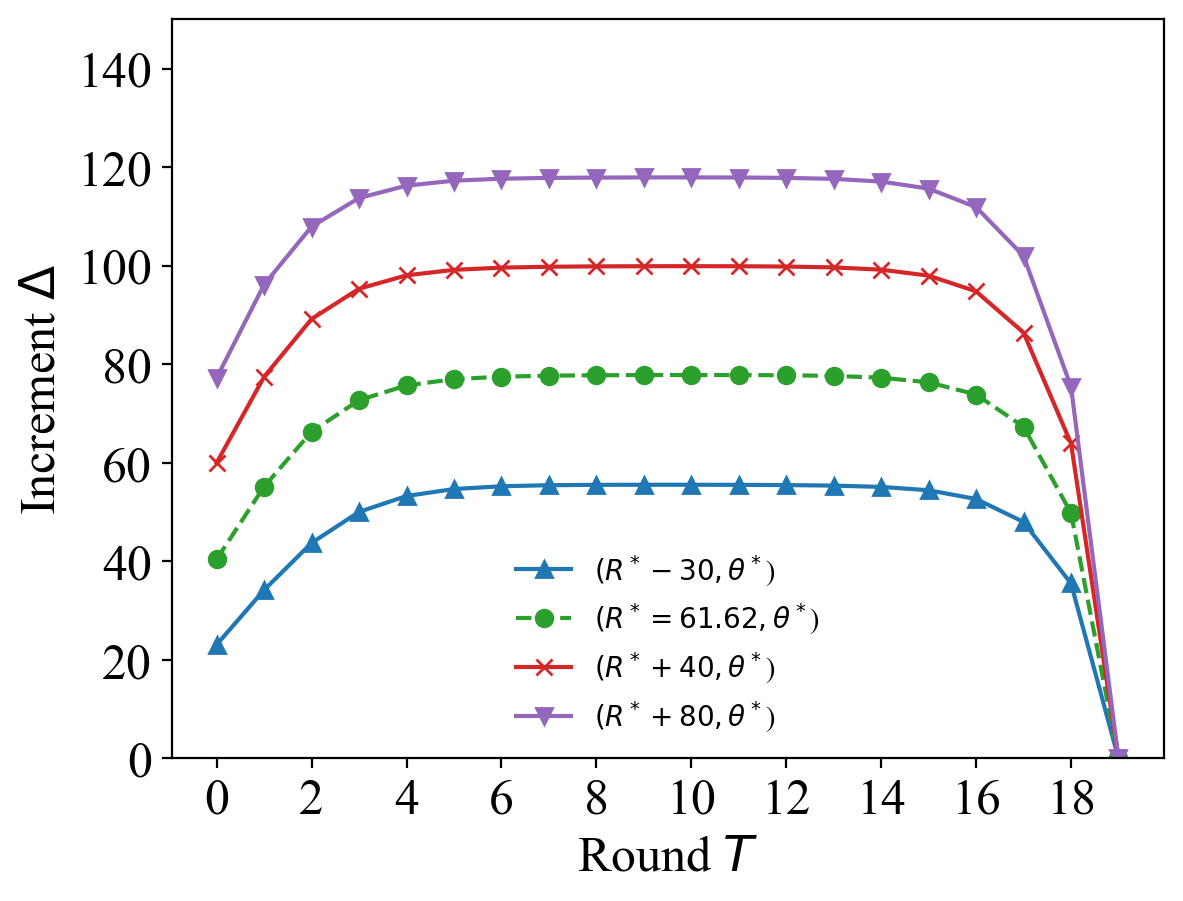
\includegraphics[width=\textwidth]{figures/figure_71_B.png}}
	\end{minipage}
	\caption{Comparative analysis of increment $\Delta_k(t)$ against a particular client $k$ versus communication rounds $t$ across various value of $\theta$ ranging from $0$ to $1$ (\textbf{left}) and $R$ ranging from $0$ to $150$ (\textbf{right}).}
  \label{fig:server_increment}
\end{figure}

\begin{figure}
	\begin{minipage}{0.49\linewidth}
		\centerline{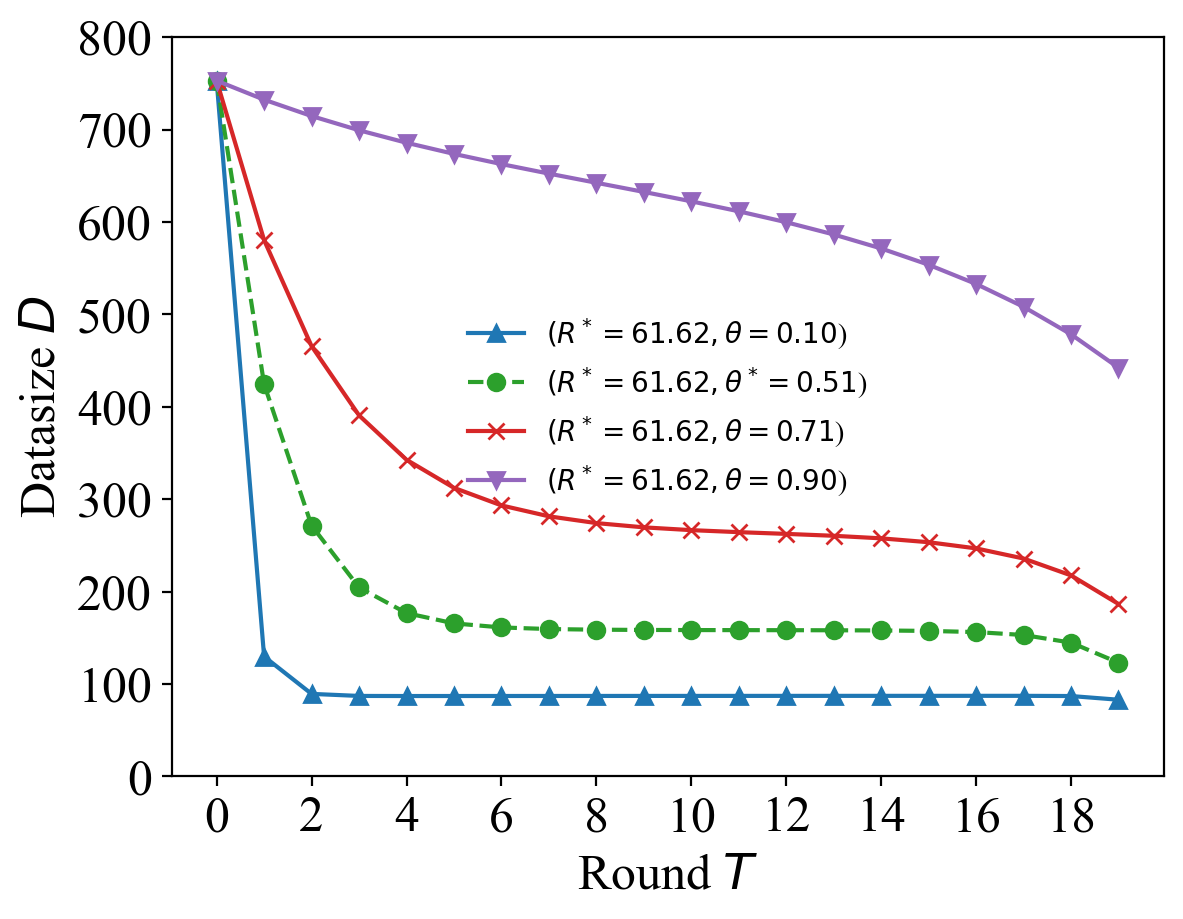
\includegraphics[width=\textwidth]{figures/figure_63_B.png}}
	\end{minipage}
	\begin{minipage}{0.49\linewidth}
		\centerline{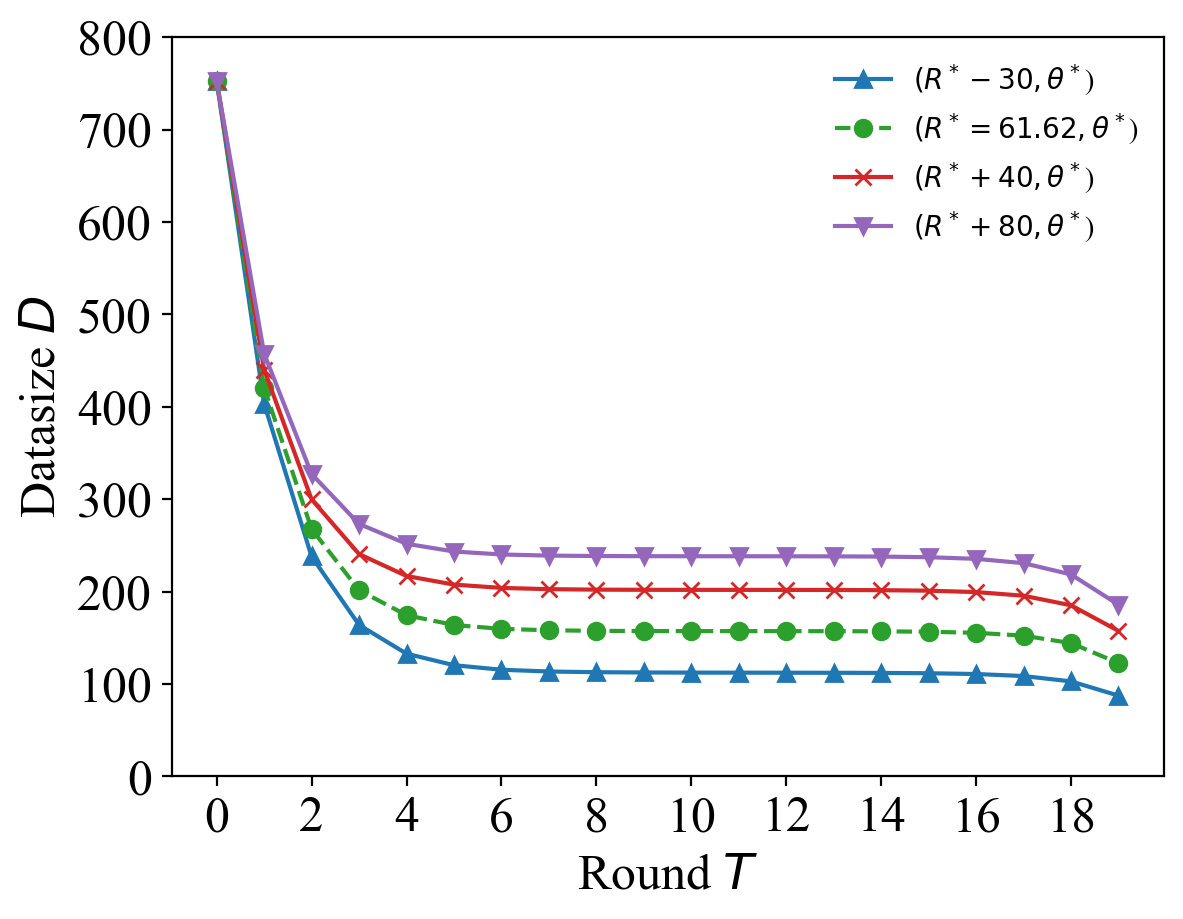
\includegraphics[width=\textwidth]{figures/figure_72_B.png}}
	\end{minipage}
	\caption{Comparative analysis of data size $D_k(t)$ against a particular client $k$ versus communication rounds $t$ across various value of $\theta$ ranging from $0$ to $1$ (\textbf{left}) and $R$ ranging from $0$ to $150$ (\textbf{right}).}
  \label{fig:server_datasize}
\end{figure}

\begin{figure}
	\begin{minipage}{0.49\linewidth}
		\centerline{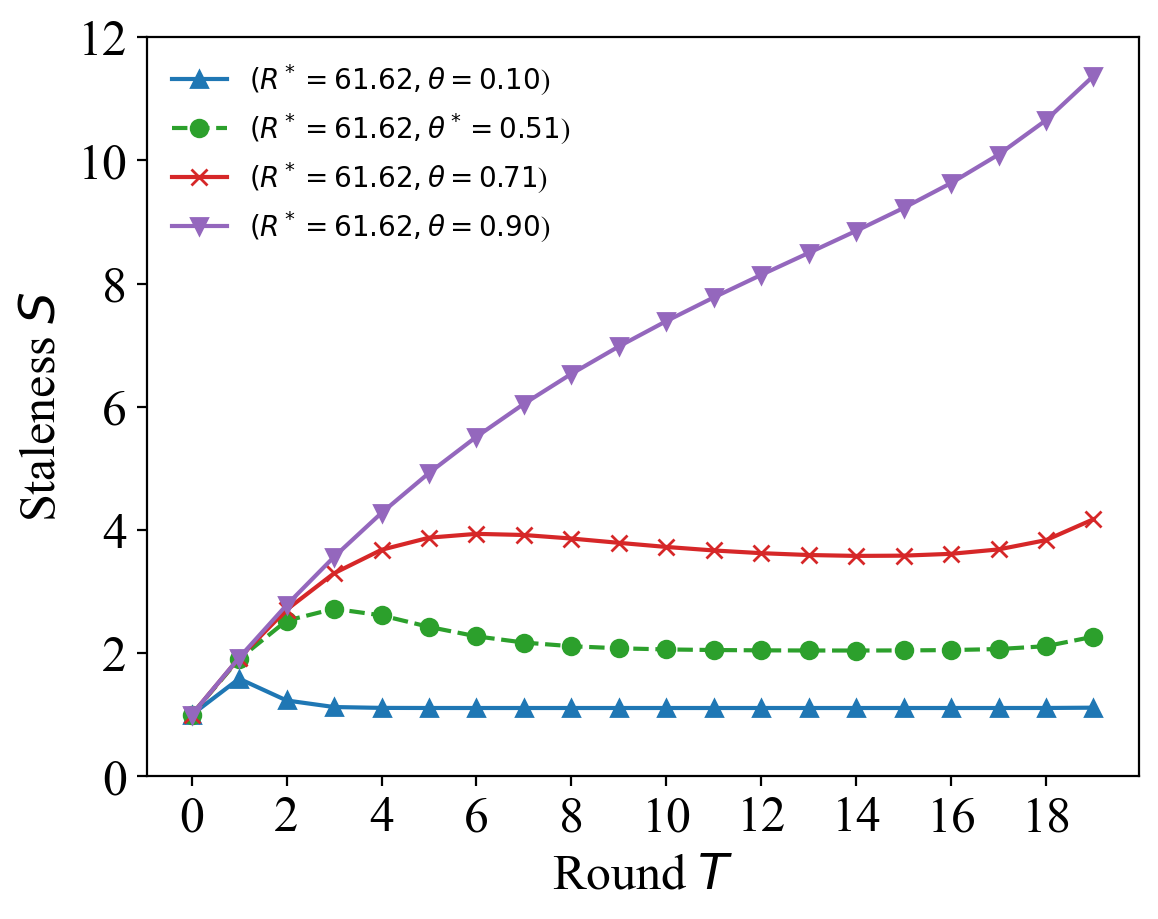
\includegraphics[width=\textwidth]{figures/figure_64_B.png}}
	\end{minipage}
	\begin{minipage}{0.49\linewidth}
		\centerline{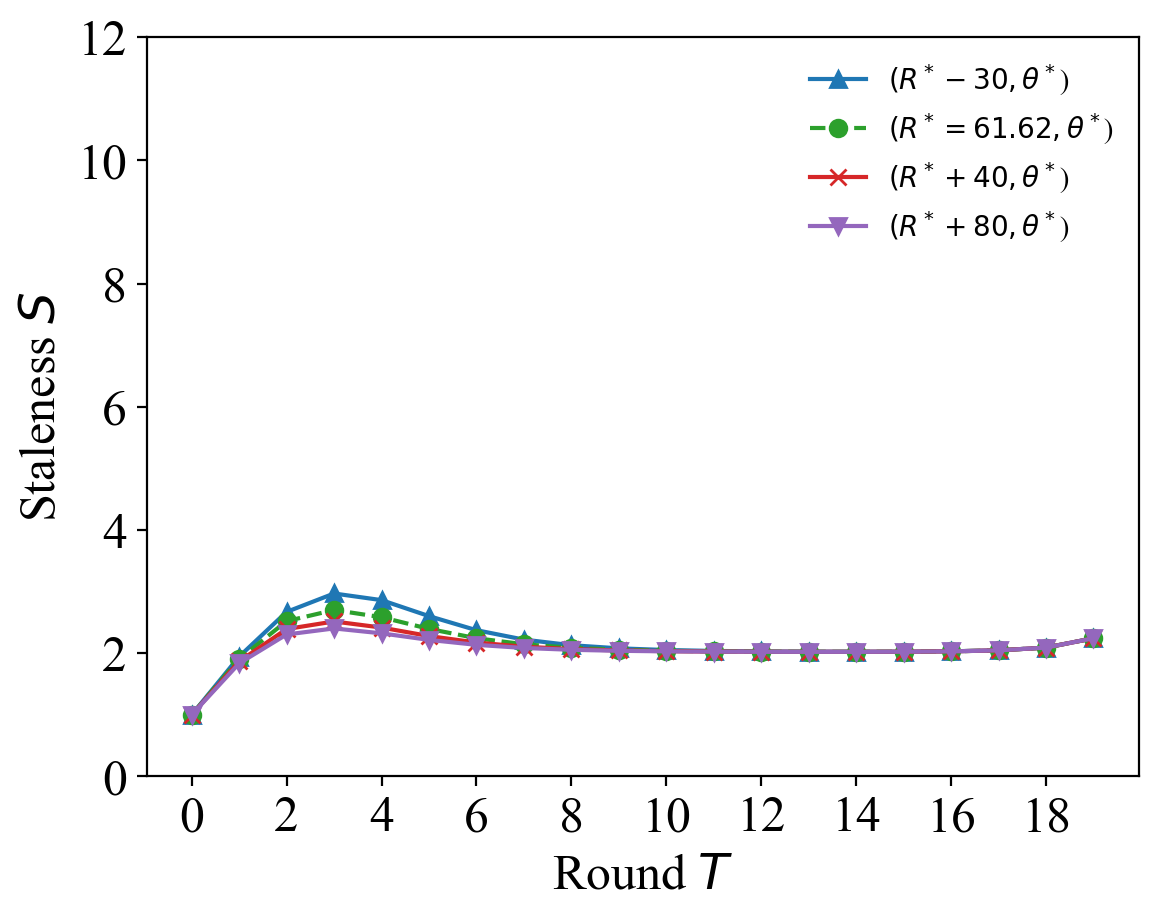
\includegraphics[width=\textwidth]{figures/figure_73_B.png}}
	\end{minipage}
	\caption{Comparative analysis of data staleness $S_k(t)$ against a particular client $k$ versus communication rounds $t$ across various value of $\theta$ ranging from $0$ to $1$ (\textbf{left}) and $R$ ranging from $0$ to $150$ (\textbf{right}).}
  \label{fig:server_staleness}
\end{figure}


\textbf{Effect of Server's Strategy on its Cost: }
In this paragraph, we analyse the effect of server's strategy $(R, \theta)$ on its cost.
Under the hyperparameters settings in experimental setup, the optimal strategy is $\pi^* = (61.62, 0.51)$.
For comparison, we fix the optimal reward $R^*$ and consider three types of strategies: $\pi_1=(R^*, \theta^*-0.4), \pi_2=(R^*, \theta^*+0.2), \pi_3=(R^*, \theta^*+0.4)$.
Besides, we also fix the optimal theta $\theta^*$ and consider another three types of strategies: $\pi_4=(R^* - 30), \pi_5=(R^*, \theta^*+40), \pi_6=(R^*, \theta+80)$.

The effect of $\theta$ and $R$ on test accuracy and cost is shown in Figure \ref{fig:server_cost_mnist} and \ref{fig:server_cost_fmnist}.
We can find that $\pi^*$(solid line) outperforms $\pi_1, \pi_2$ and $\pi_3$(dotted line) in terms of test accuracy on the MNIST and CIFAR-10 datasets. The underlying reason is that strategy $\pi_2, \pi_3$ with improperly great $\theta$ contributes to huge but stale buffer data, while $\pi_1$ with improperly small $\theta$ contributes to fresh but tiny ones. Both of them leads to worse model performance.
Under the same payment to clients, $\pi^*$ reach the lowest cost compared with other strategies.

In addition, $\pi_5$ and $\pi_6$(dotted line) surpass the optimal strategy of $\pi^*$(solid line) with respect to test accuracy across all datasets because richer payment encourages clients to collect more fresh data, thereby enhance the model performance.
However, $\pi^*$ still reach the lowest cost, which indicates that our proposed strategy has the ability to strike the trade-off between payment and accuracy loss simultaneously.
The above two experiments verify the optimality of our proposed strategy.

\begin{figure}
	\begin{minipage}{0.49\linewidth}
		\centerline{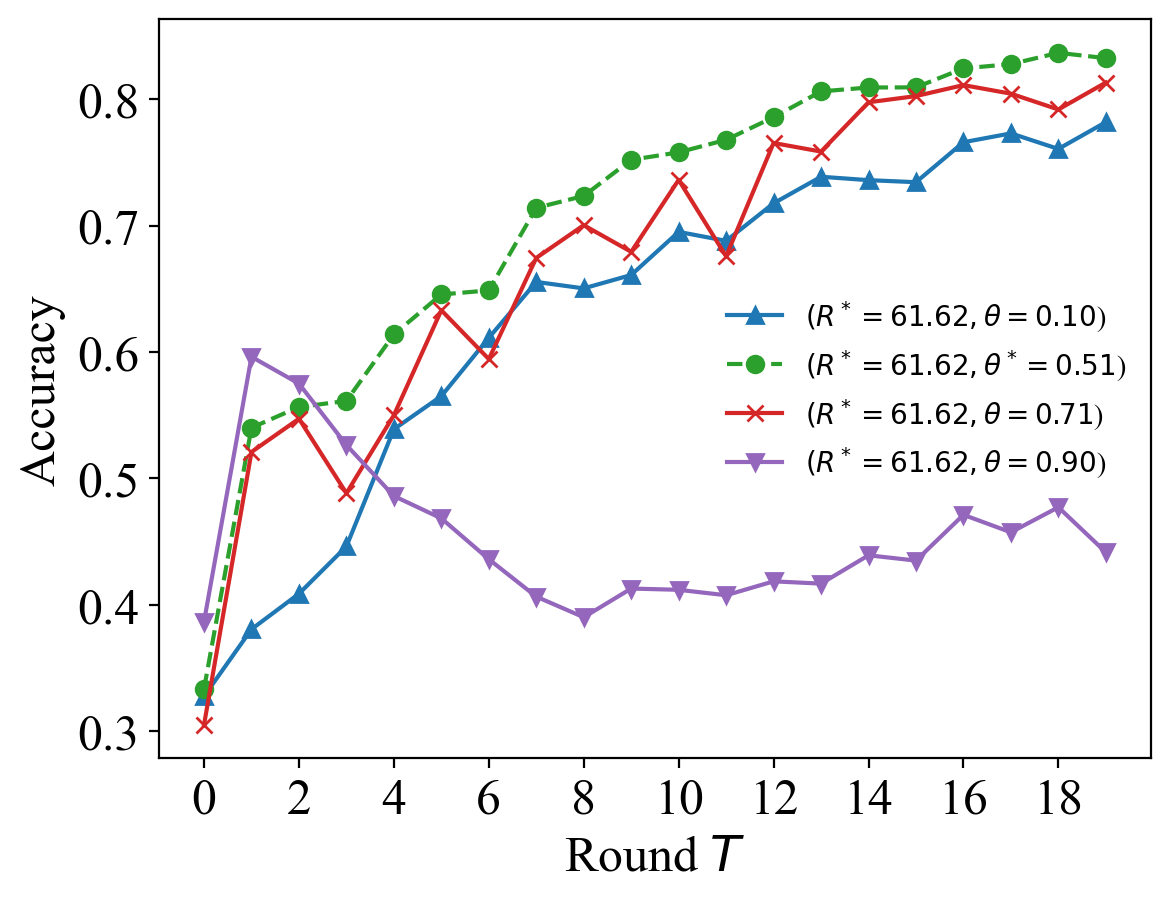
\includegraphics[width=\textwidth]{figures/figure_65_B.png}}
	\end{minipage}
	\begin{minipage}{0.49\linewidth}
		\centerline{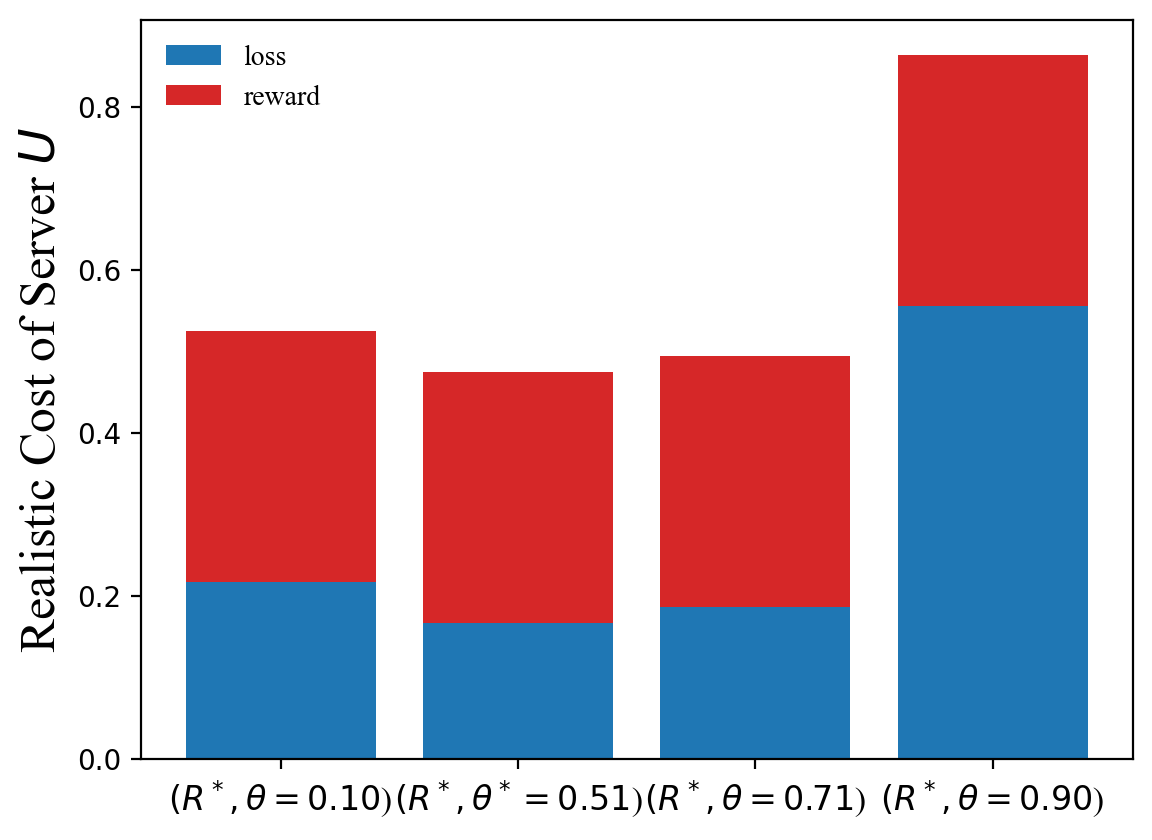
\includegraphics[width=\textwidth]{figures/figure_66_B.png}}
	\end{minipage}
	\begin{minipage}{0.49\linewidth}
		\centerline{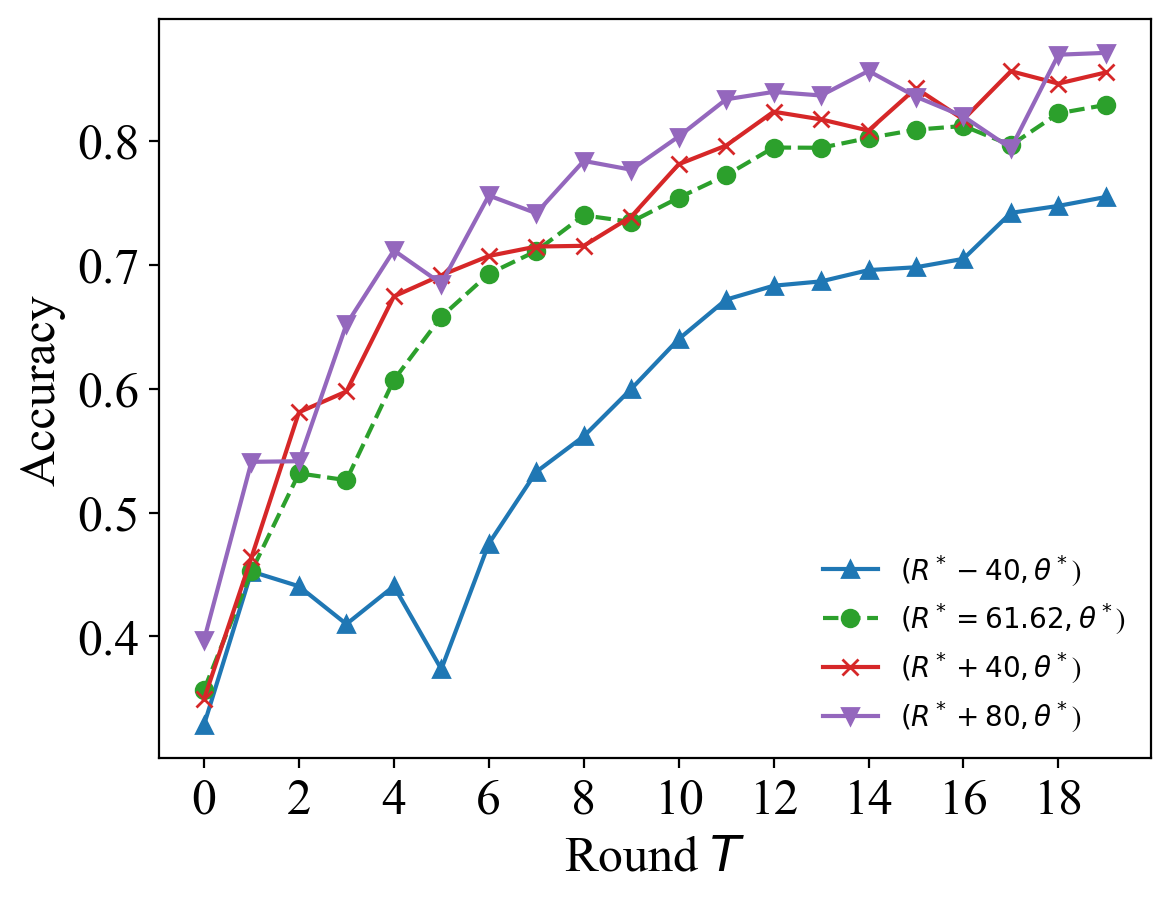
\includegraphics[width=\textwidth]{figures/figure_74_B.png}}
	\end{minipage}
	\begin{minipage}{0.49\linewidth}
		\centerline{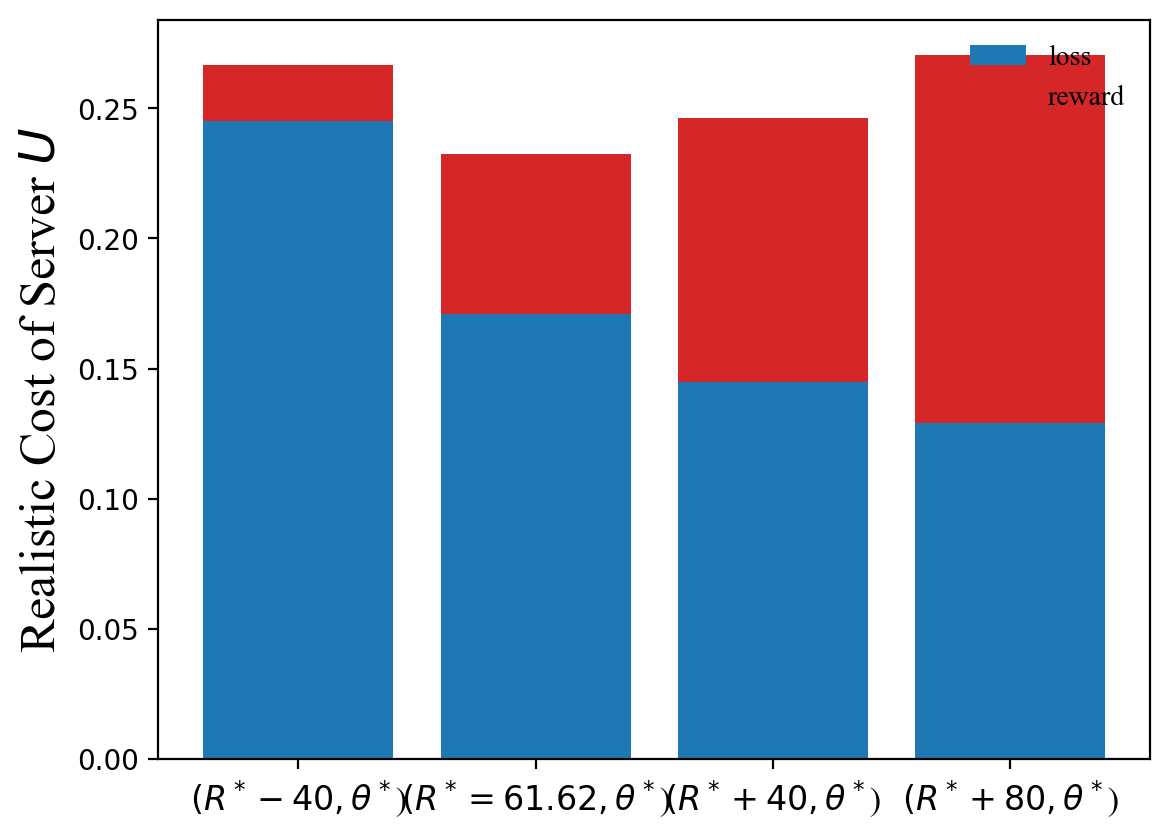
\includegraphics[width=\textwidth]{figures/figure_75_B.png}}
	\end{minipage}
	\caption{Comparative analysis of test accuracy (\textbf{left}) and cost (\textbf{right}) versus communication rounds $t$ across various value of $\theta$ ranging from $0$ to $1$(\textbf{top}) and $R$ ranging from $0$ to $140$(\textbf{bottom}) with CNN over MNIST. Left-Top: Test accuracy vs. Rounds, Right-Top: Cost vs. Rounds}
  \label{fig:server_cost_mnist}
\end{figure}

\begin{figure}
	\begin{minipage}{0.49\linewidth}
		\centerline{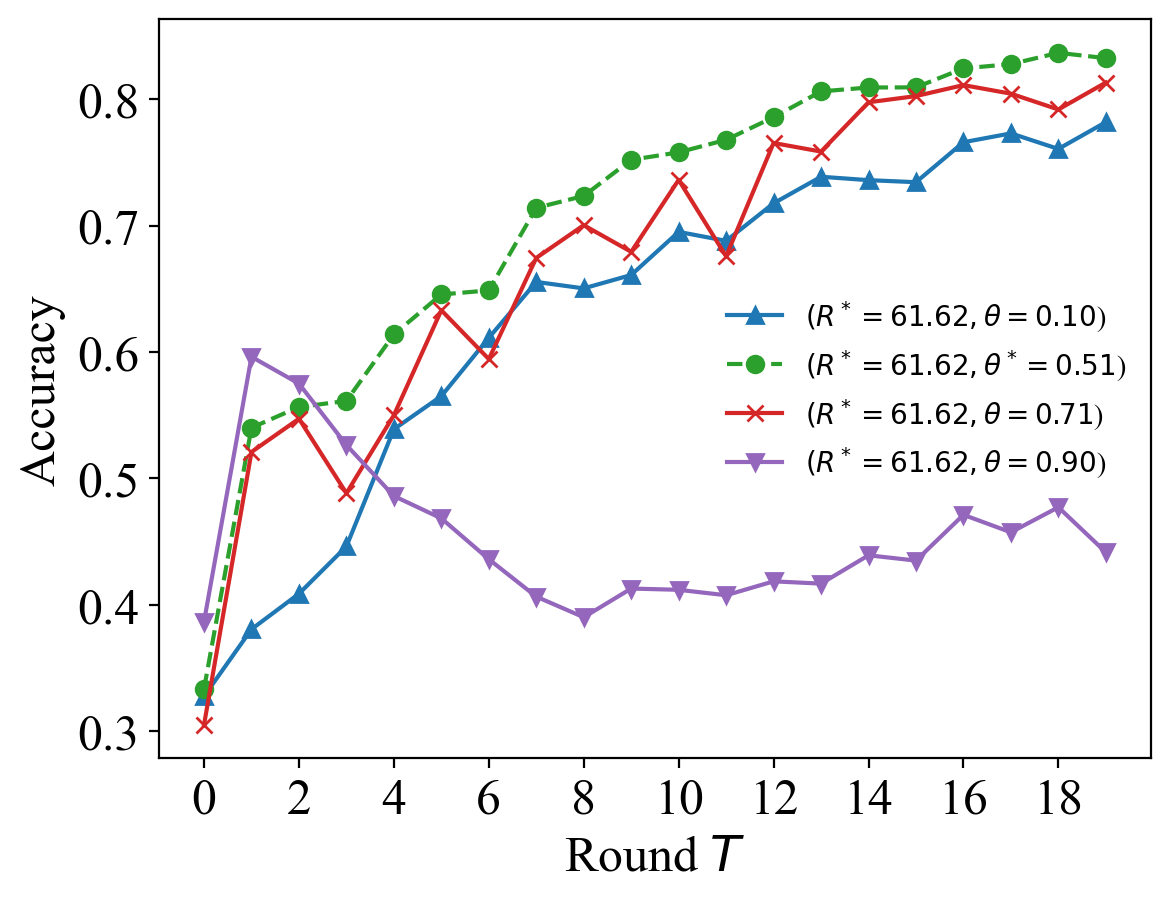
\includegraphics[width=\textwidth]{figures/figure_65_B.png}}
	\end{minipage}
	\begin{minipage}{0.49\linewidth}
		\centerline{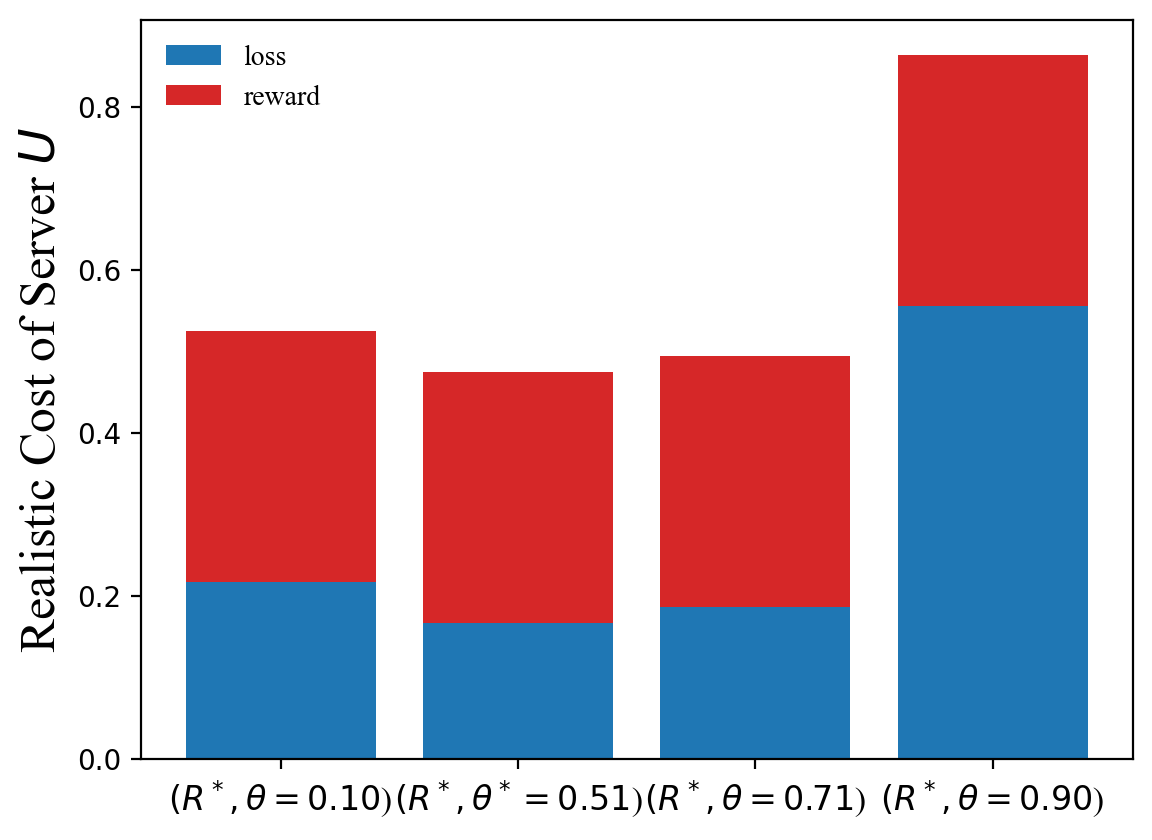
\includegraphics[width=\textwidth]{figures/figure_66_B.png}}
	\end{minipage}
	\begin{minipage}{0.49\linewidth}
		\centerline{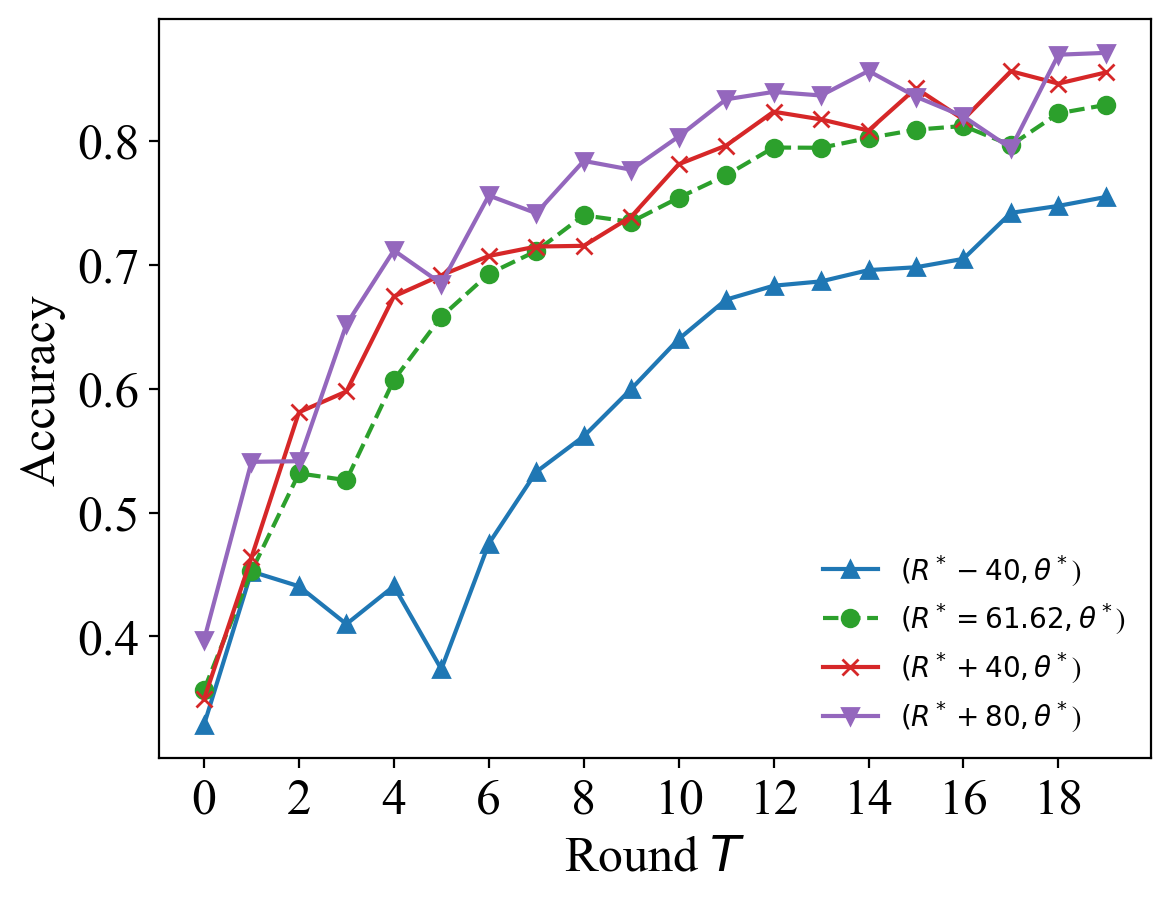
\includegraphics[width=\textwidth]{figures/figure_74_B.png}}
	\end{minipage}
	\begin{minipage}{0.49\linewidth}
		\centerline{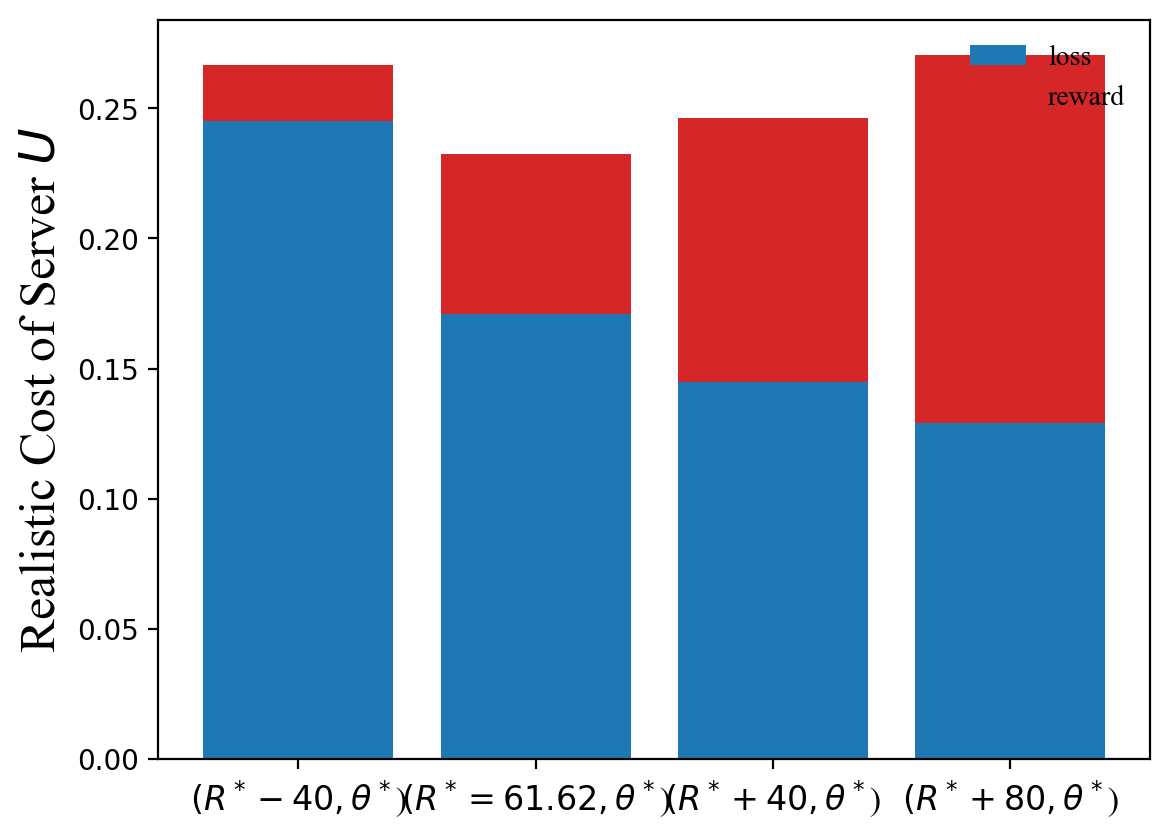
\includegraphics[width=\textwidth]{figures/figure_75_B.png}}
	\end{minipage}
	\caption{Comparative analysis of test accuracy (\textbf{left}) and cost (\textbf{right}) versus communication rounds $t$ across various value of $\theta$ ranging from $0$ to $1$(\textbf{top}) and $R$ ranging from $0$ to $140$(\textbf{bottom}) with CNN over FMNIST. Left-Top: Test accuracy vs. Rounds, Right-Top: Cost vs. Rounds}
  \label{fig:server_cost_fmnist}
\end{figure}

% \begin{figure*}[htbp] % 单栏模式
%     \centering
%     % 使用 tabular 确保对齐
%     \begin{tabular}{ccc} % 定义三列布局
%         \multicolumn{1}{c}{$\sigma=0.1$(low timeliness task)} &
%         \multicolumn{1}{c}{$\sigma=0.3$(normal timeliness task)} &
%         \multicolumn{1}{c}{$\sigma=0.7$(high timeliness task)} \\ % 顶部标题行
        
%         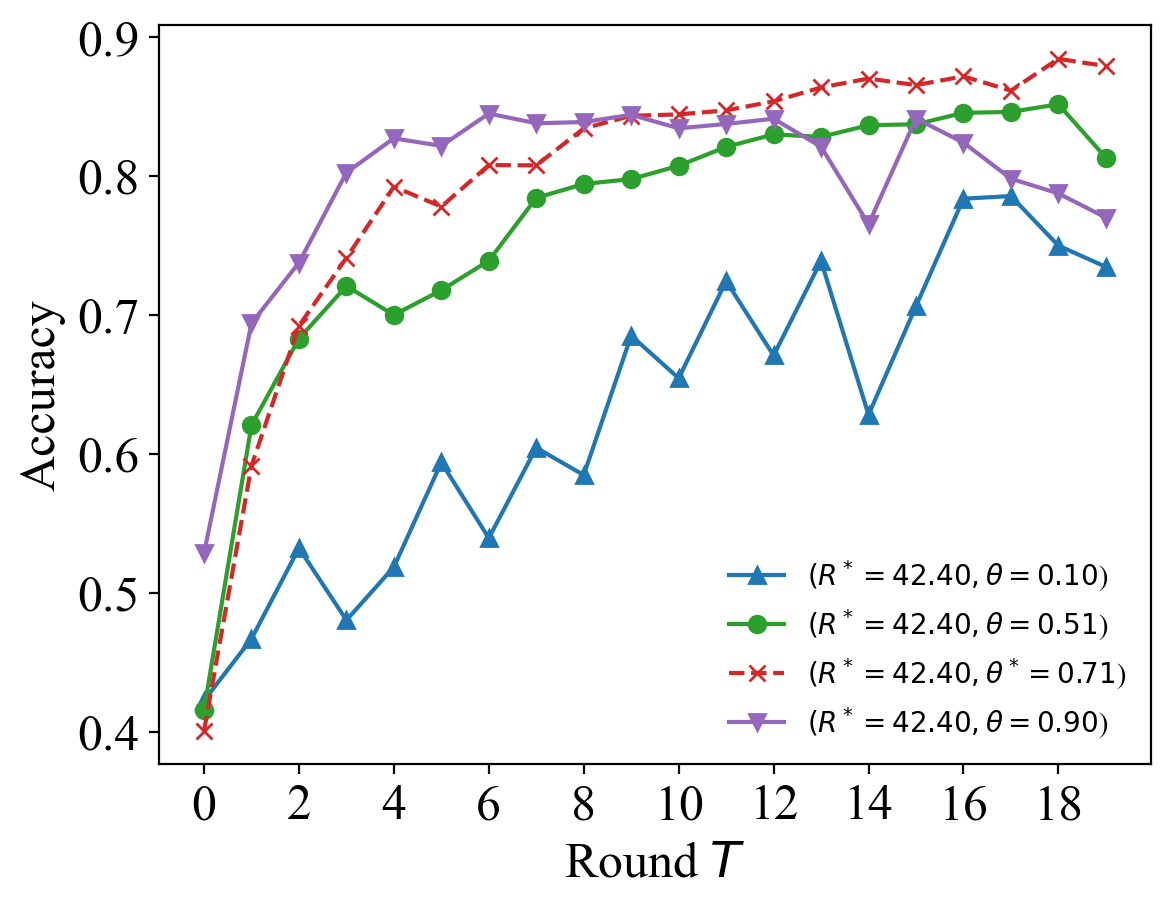
\includegraphics[width=0.3\linewidth]{figures/figure_65_A.png} &
%         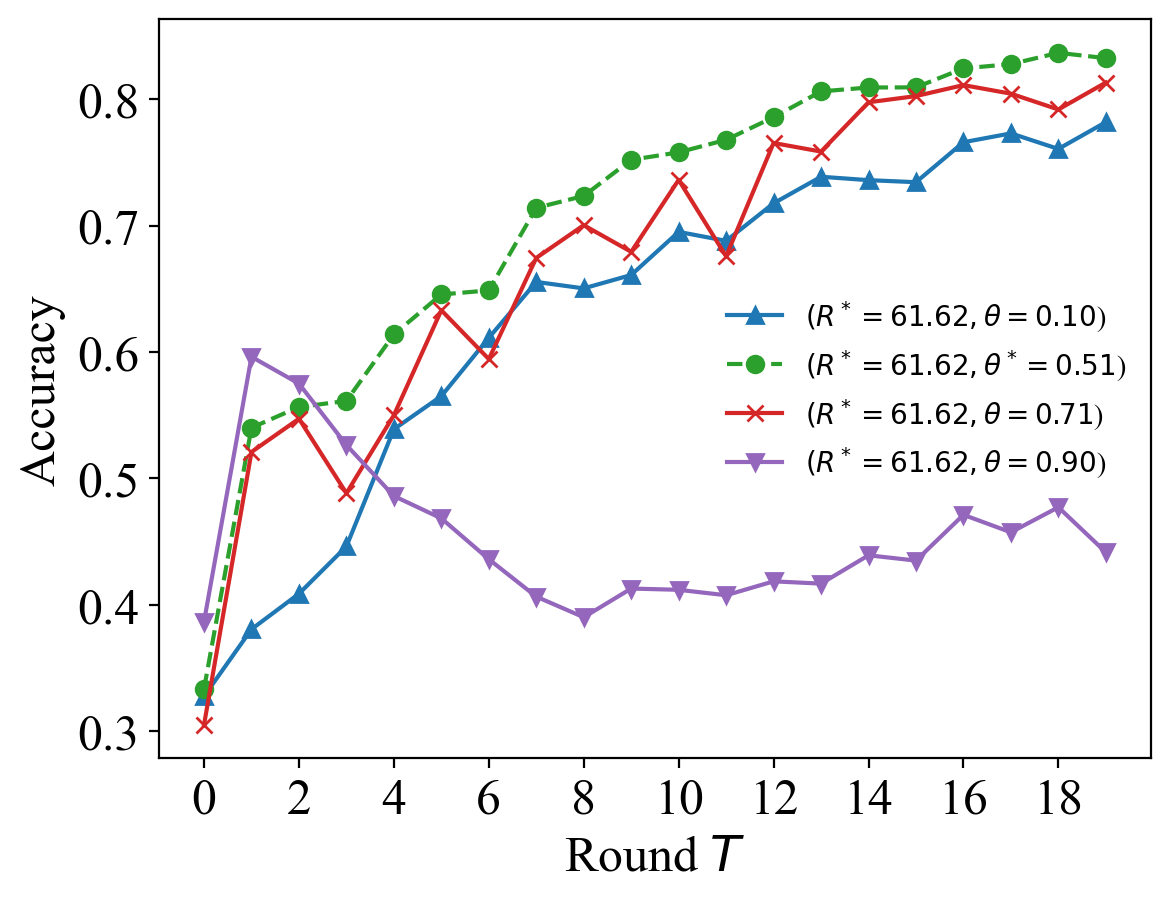
\includegraphics[width=0.3\linewidth]{figures/figure_65_B.png} &
%         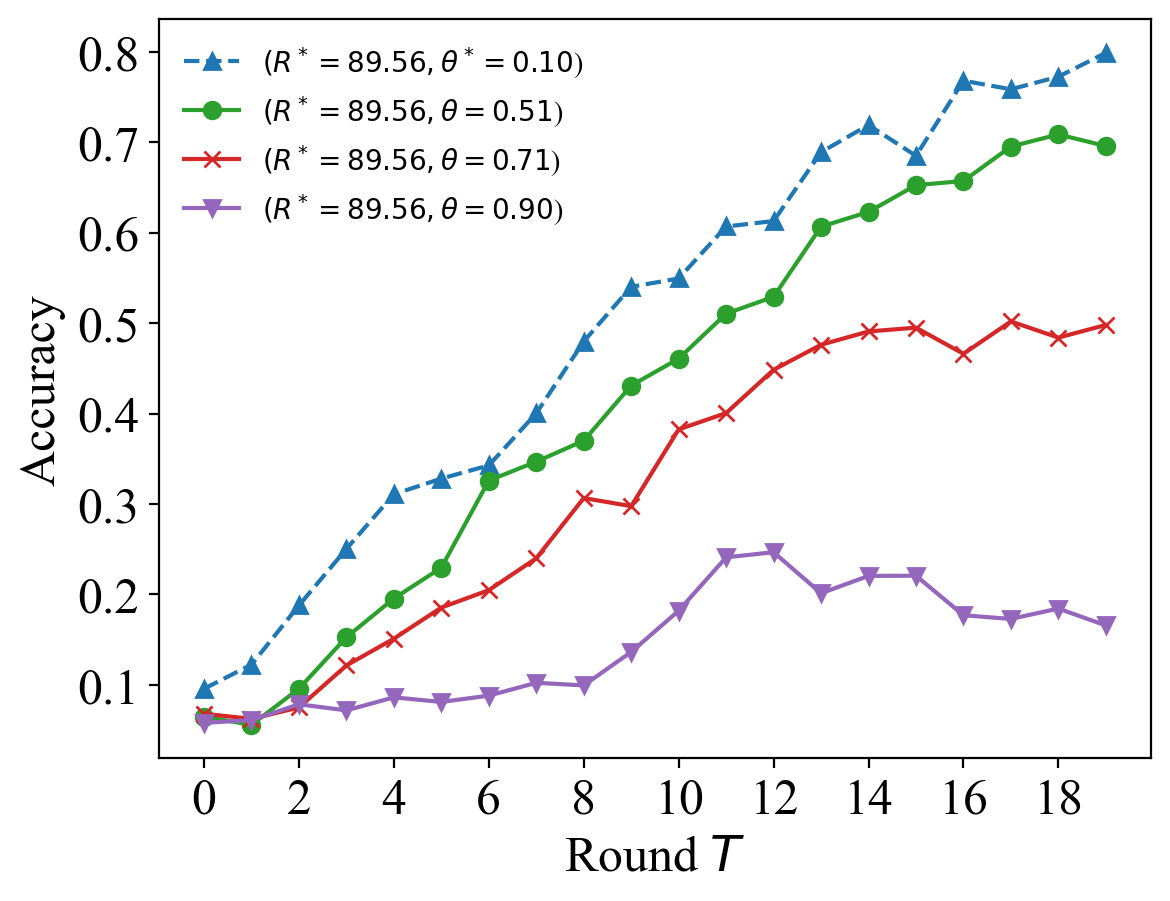
\includegraphics[width=0.3\linewidth]{figures/figure_65_C.png} \\ % 第一行图片
        
%         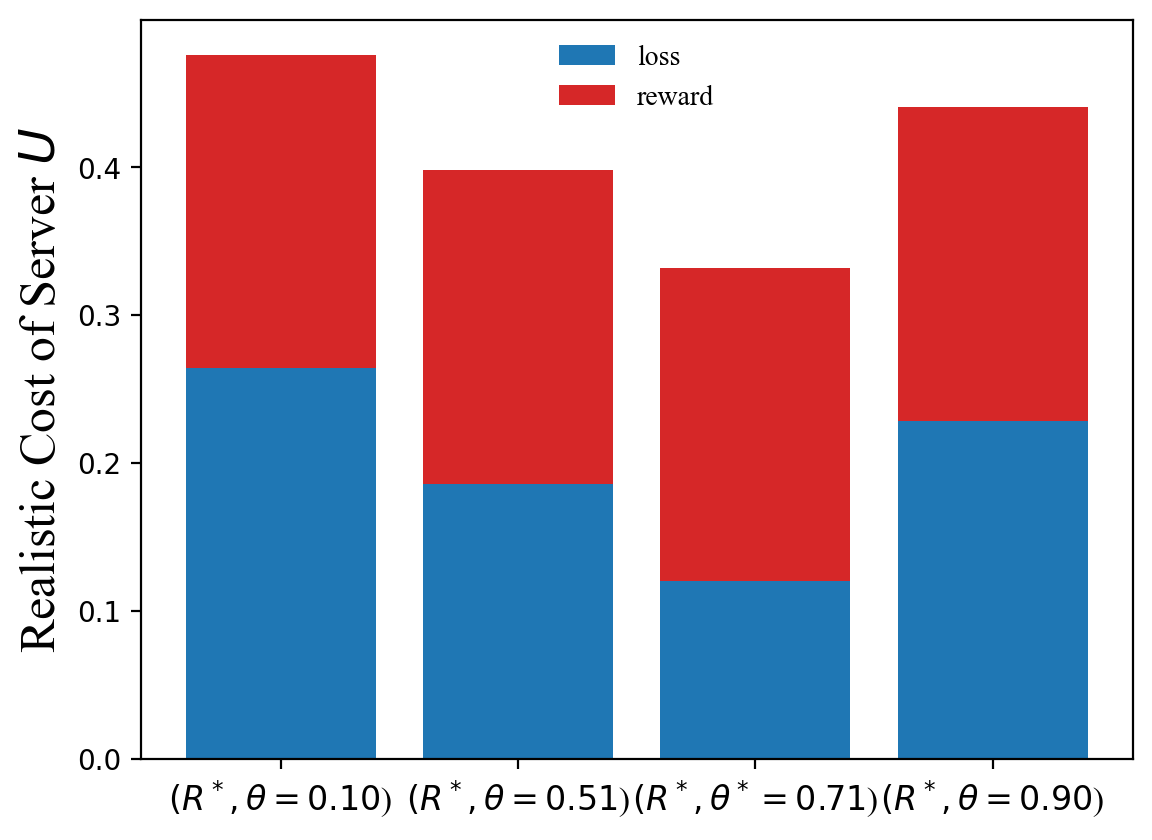
\includegraphics[width=0.3\linewidth]{figures/figure_66_A.png} &
%         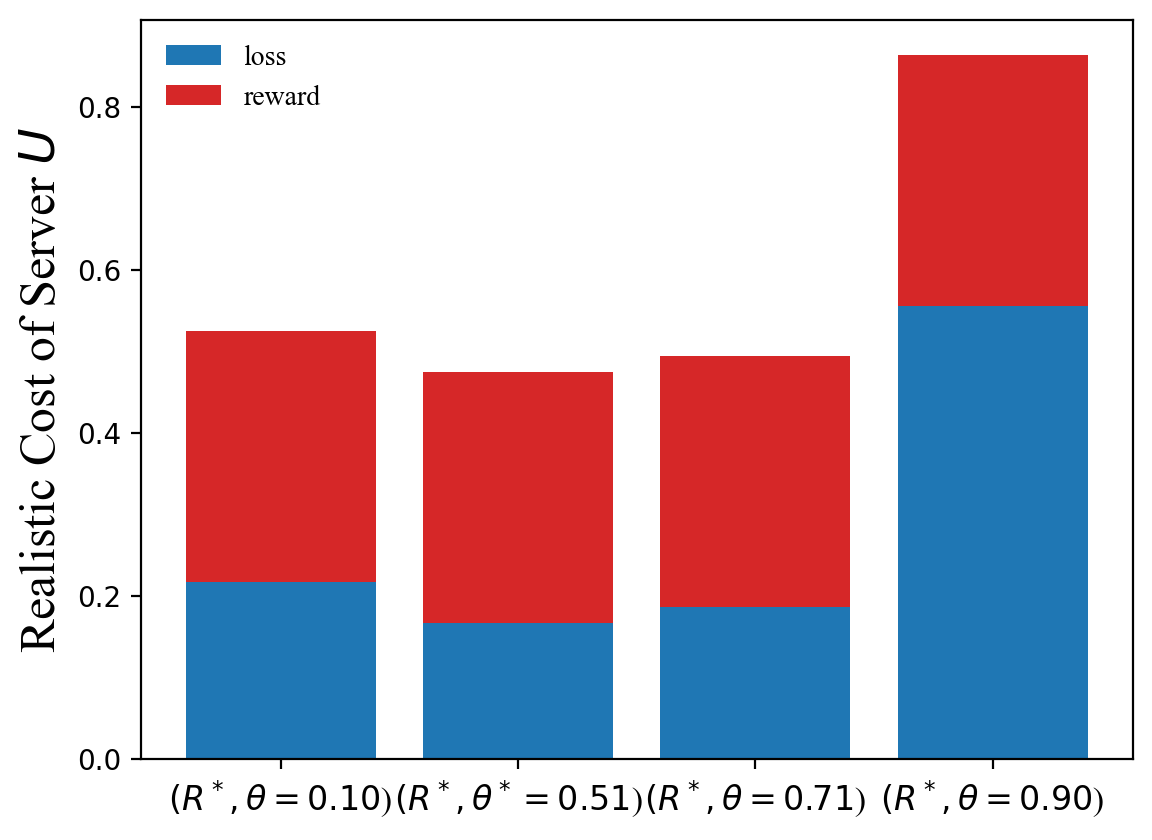
\includegraphics[width=0.3\linewidth]{figures/figure_66_B.png} &
%         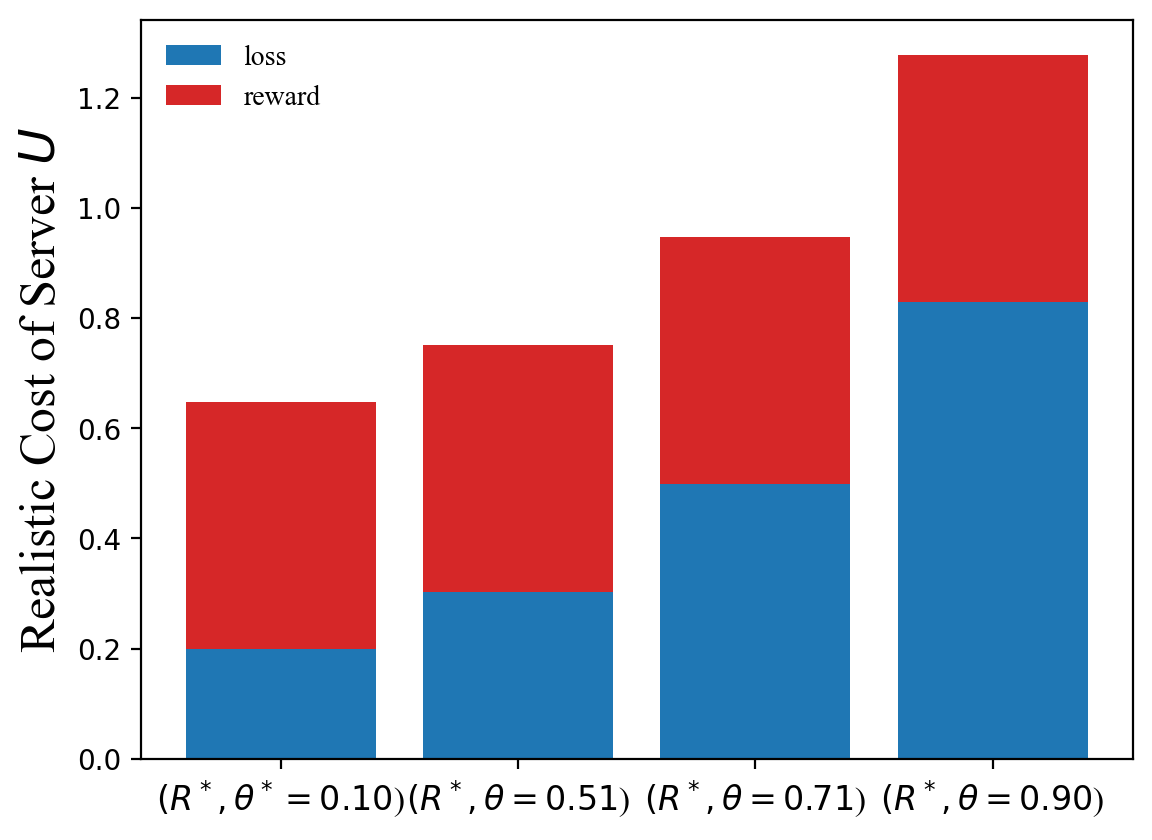
\includegraphics[width=0.3\linewidth]{figures/figure_66_C.png} \\ % 第二行图片
        
%         % \textit{Row 2, Col 1} &
%         % \textit{Row 2, Col 2} &
%         % \textit{Row 2, Col 3} \\ % 第二行描述
%     \end{tabular}
%     \caption{A 3×2 image matrix with column titles and aligned content.}
%     \label{fig:server_accuracy_theta}
% \end{figure*}

% \begin{figure*}[htbp] % 单栏模式
%   \centering
  
%   % 使用 tabular 确保对齐
%   \begin{tabular}{ccc} % 定义三列布局
%       \multicolumn{1}{c}{$\sigma=0.1$(low timeliness task)} &
%       \multicolumn{1}{c}{$\sigma=0.3$(normal timeliness task)} &
%       \multicolumn{1}{c}{$\sigma=0.7$(high timeliness task)} \\ % 顶部标题行
      
%       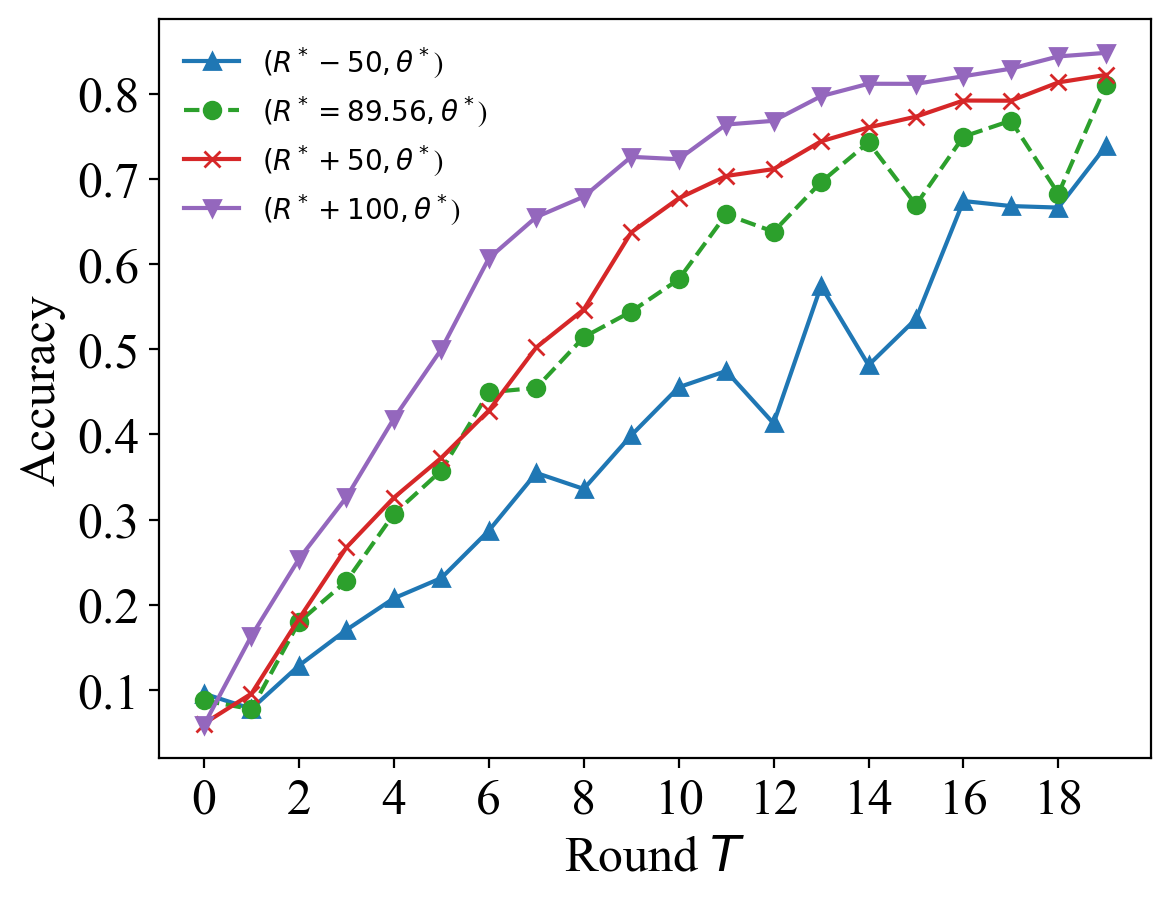
\includegraphics[width=0.3\linewidth]{figures/figure_74_A.png} &
%       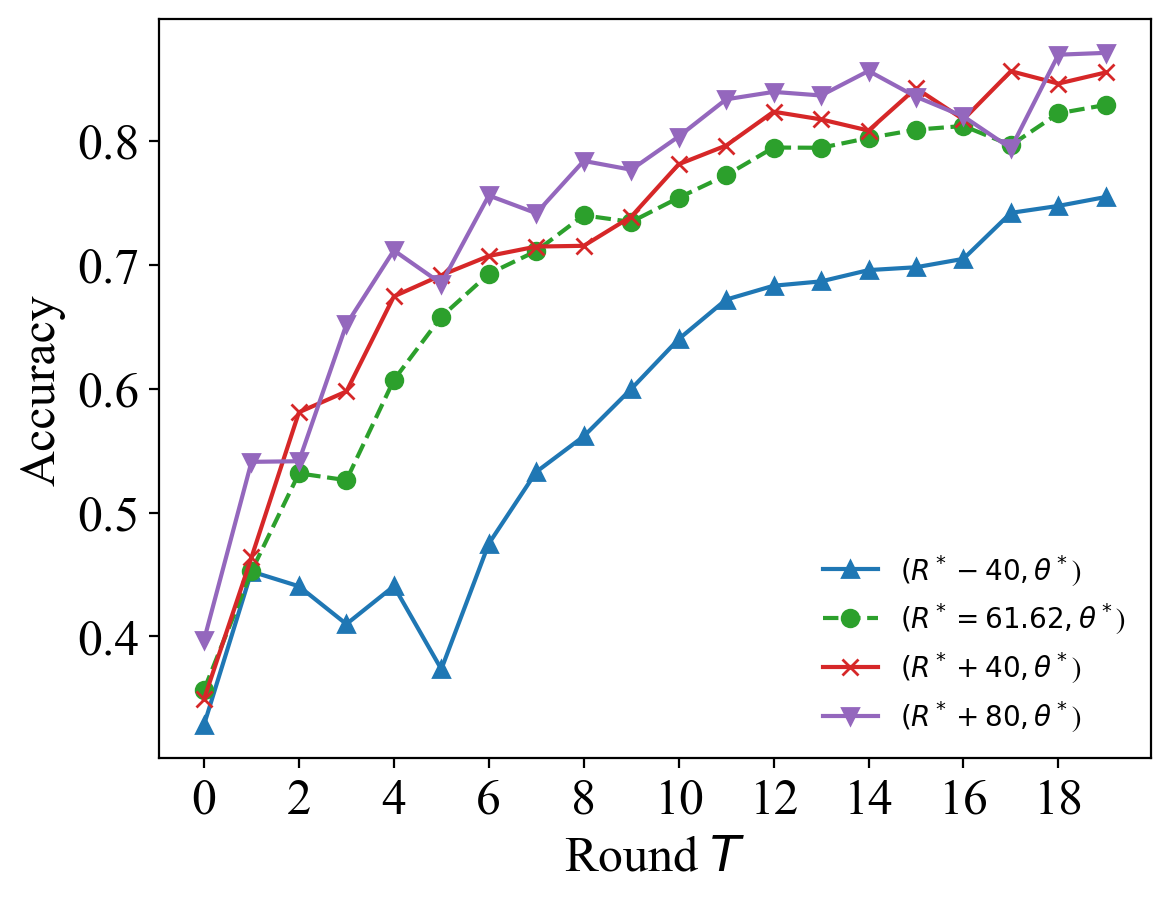
\includegraphics[width=0.3\linewidth]{figures/figure_74_B.png} &
%       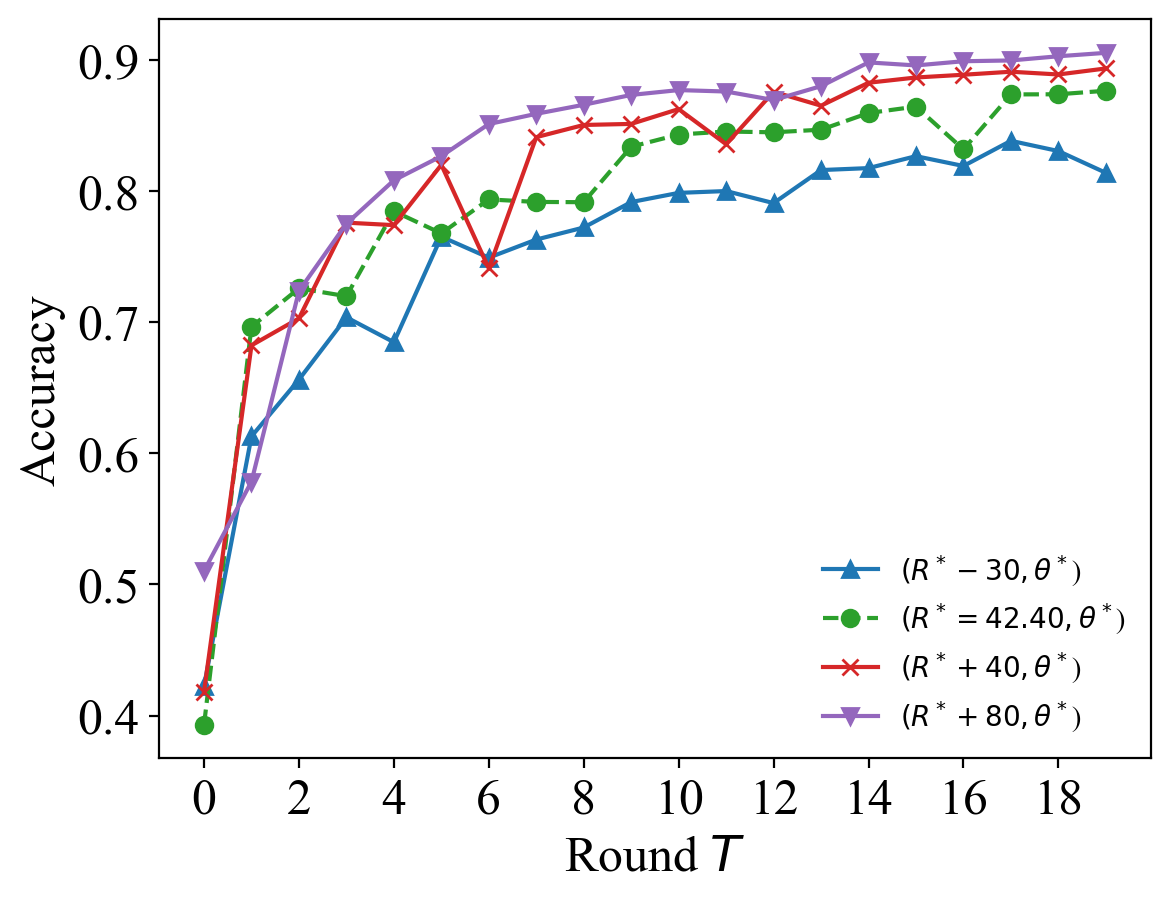
\includegraphics[width=0.3\linewidth]{figures/figure_74_C.png} \\ % 第一行图片
      
%       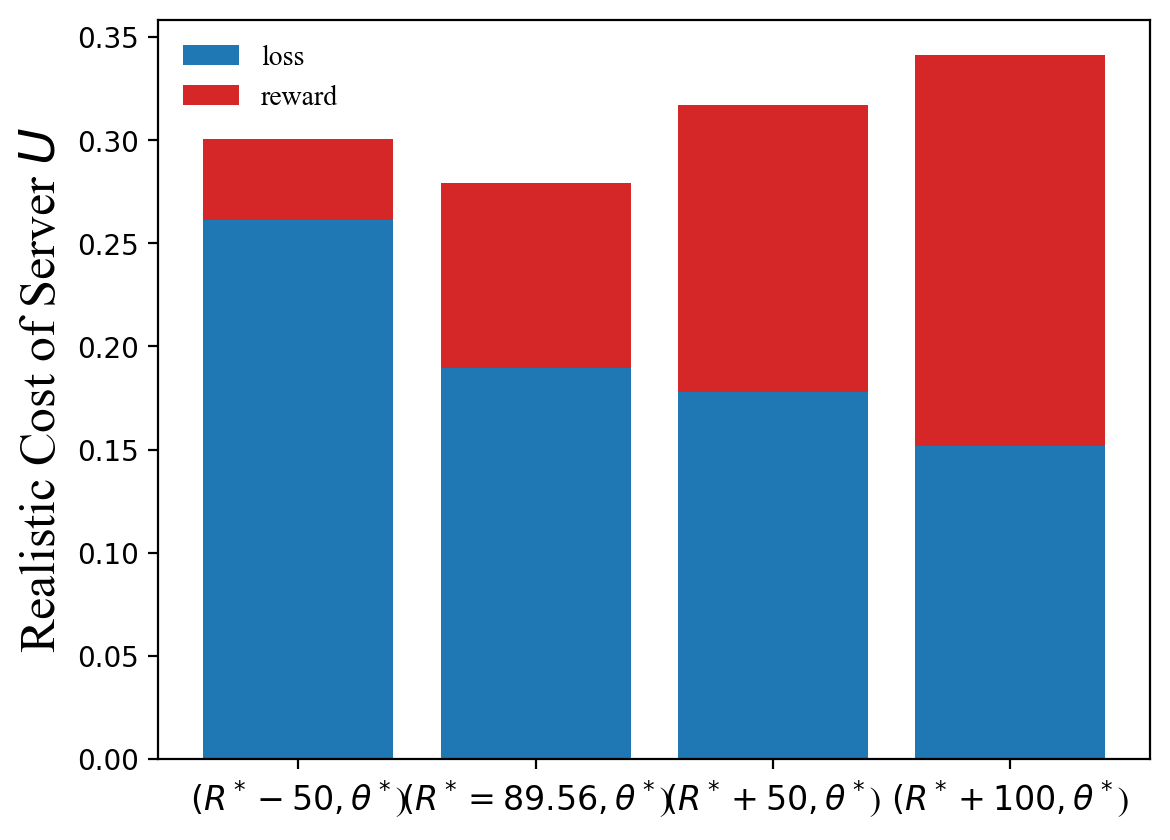
\includegraphics[width=0.3\linewidth]{figures/figure_75_A.png} &
%       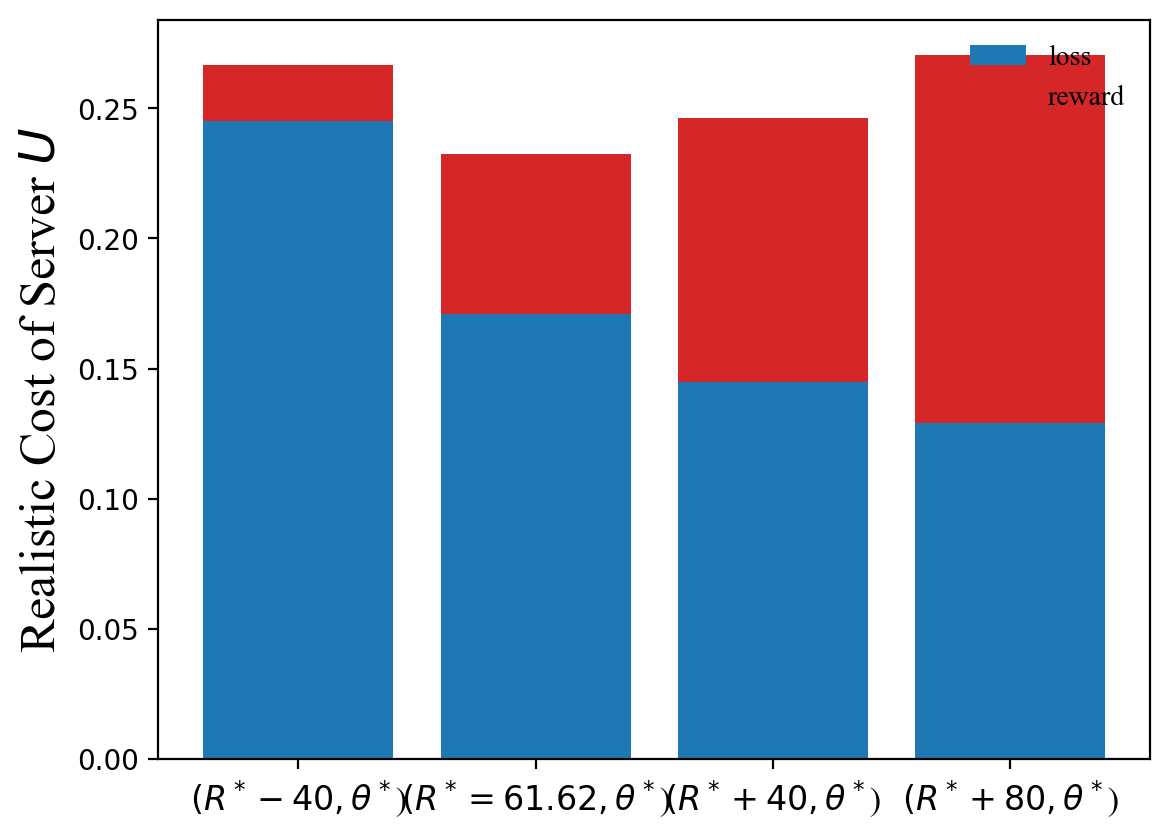
\includegraphics[width=0.3\linewidth]{figures/figure_75_B.png} &
%       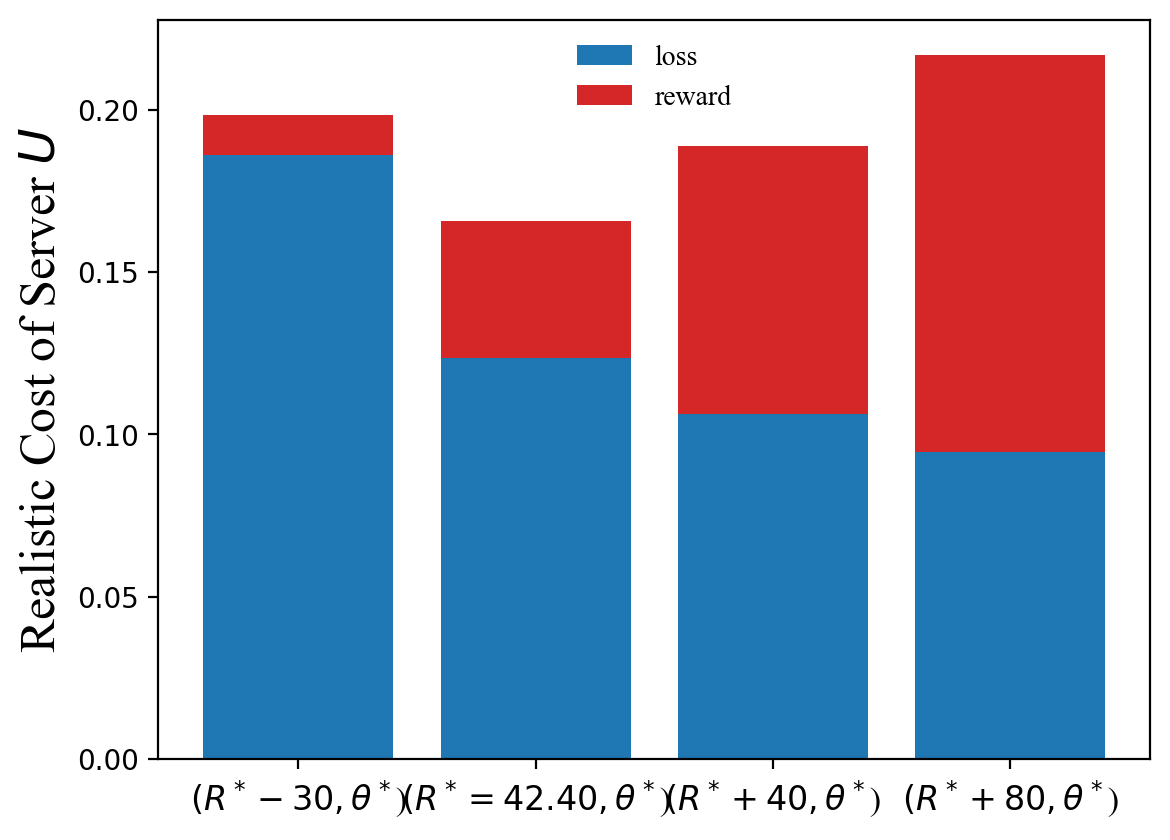
\includegraphics[width=0.3\linewidth]{figures/figure_75_C.png} \\ % 第二行图片
      
%       % \textit{Row 2, Col 1} &
%       % \textit{Row 2, Col 2} &
%       % \textit{Row 2, Col 3} \\ % 第二行描述
%   \end{tabular}
  
%   \caption{A 3×2 image matrix with column titles and aligned content.}
%   \label{fig:server_accuracy_reward}
% \end{figure*}

% \begin{figure*}
% 	\begin{subfigure}{0.31\textwidth}
% 		\centering
%     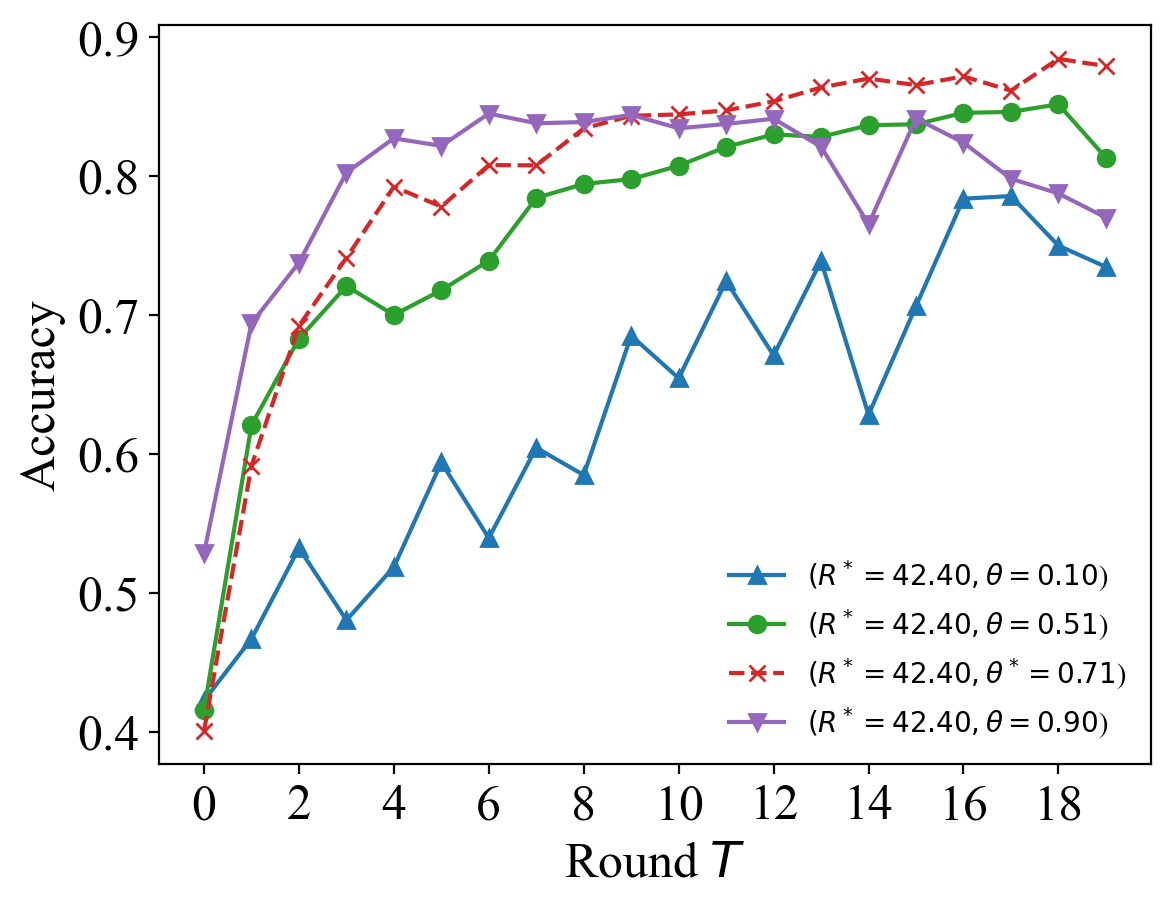
\includegraphics[width=\textwidth]{figures/figure_65_A.png}
%     \caption{$\sigma=0.1$}
% 	\end{subfigure}
%   \quad
% 	\begin{subfigure}{0.31\textwidth}
% 		\centering
% 		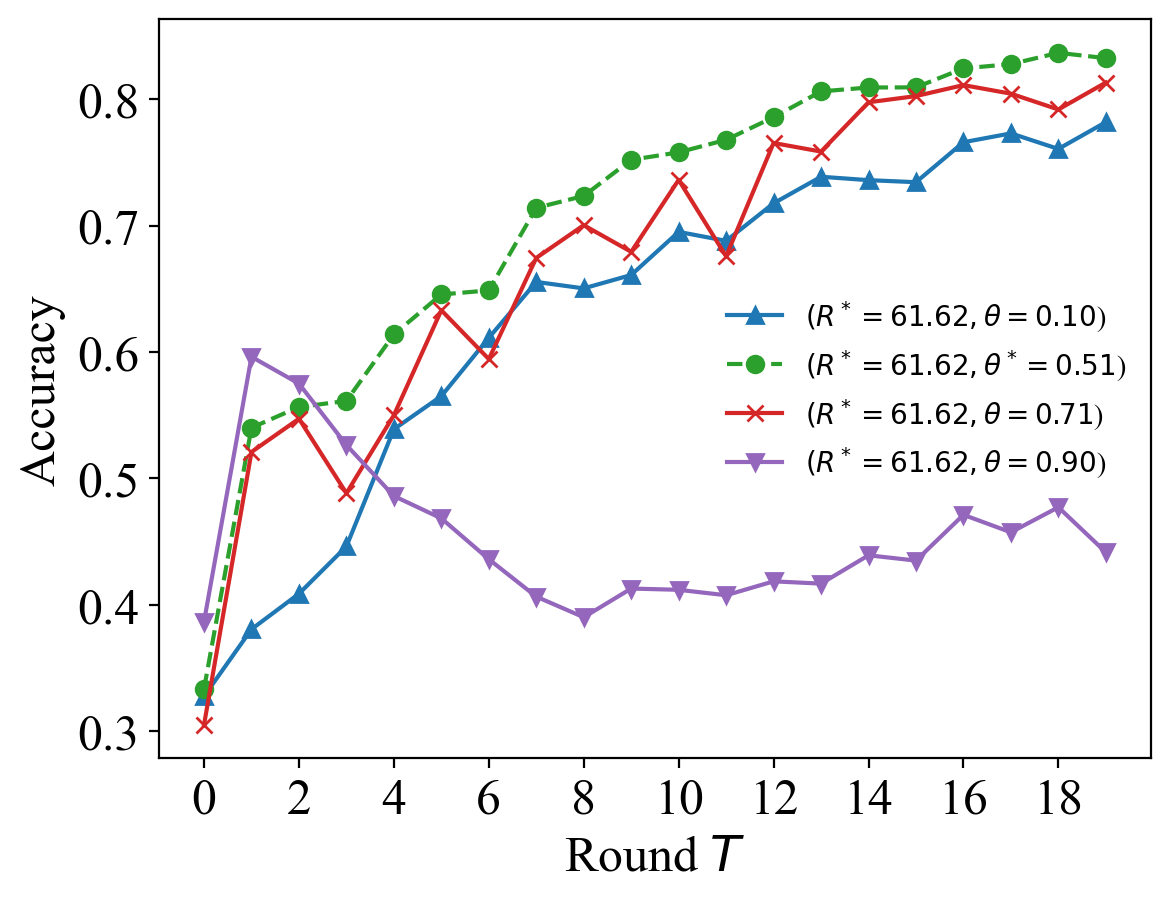
\includegraphics[width=\textwidth]{figures/figure_65_B.png}
%     \caption{$\sigma=0.3$}
% 	\end{subfigure}
%   \quad
%   \begin{subfigure}{0.31\textwidth}
% 		\centering
% 		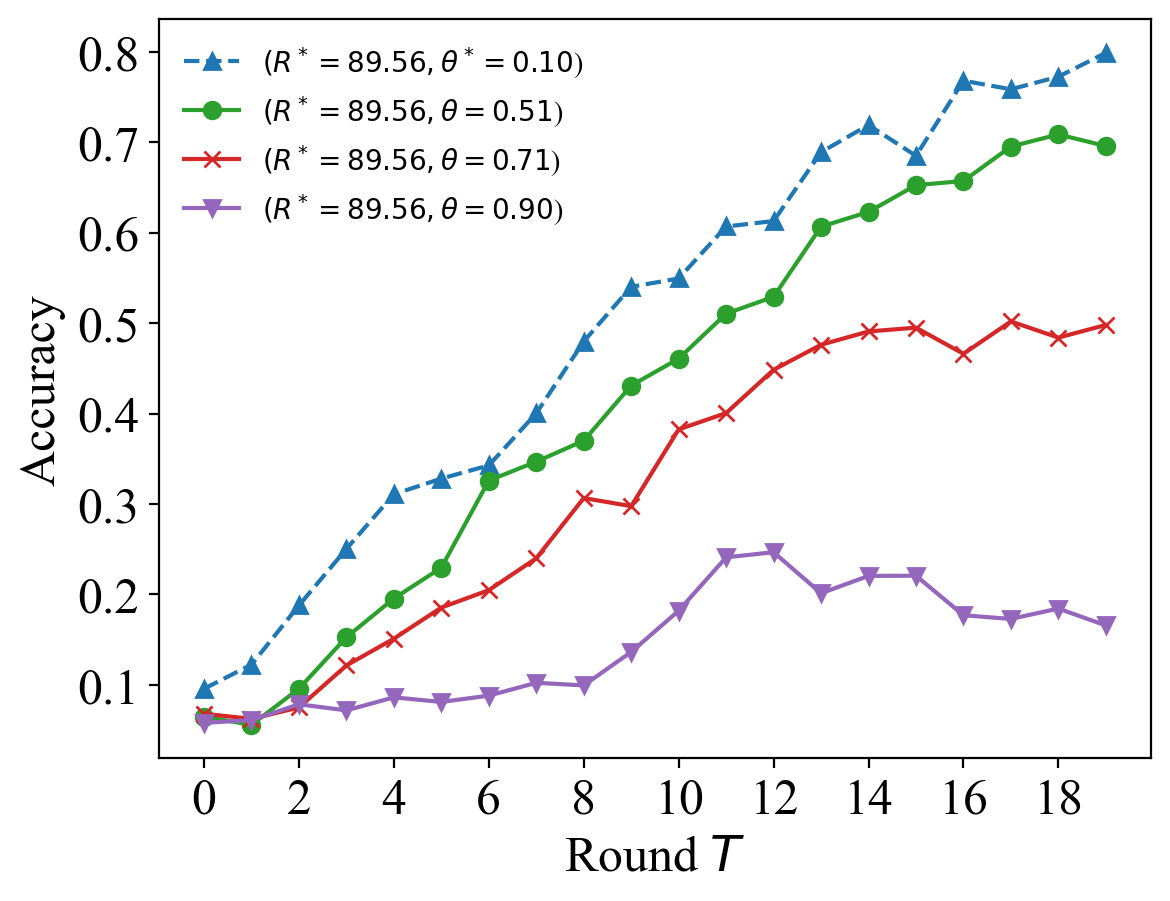
\includegraphics[width=\textwidth]{figures/figure_65_C.png}
%     \caption{$\sigma=0.7$}
% 	\end{subfigure}
% 	\caption{The effect of $\theta$ on model performance}
% \end{figure*}

% \textit{Effect of initiative data on server' cost:}
% \begin{figure*}
% 	\begin{subfigure}{0.31\textwidth}
% 		\centering
%     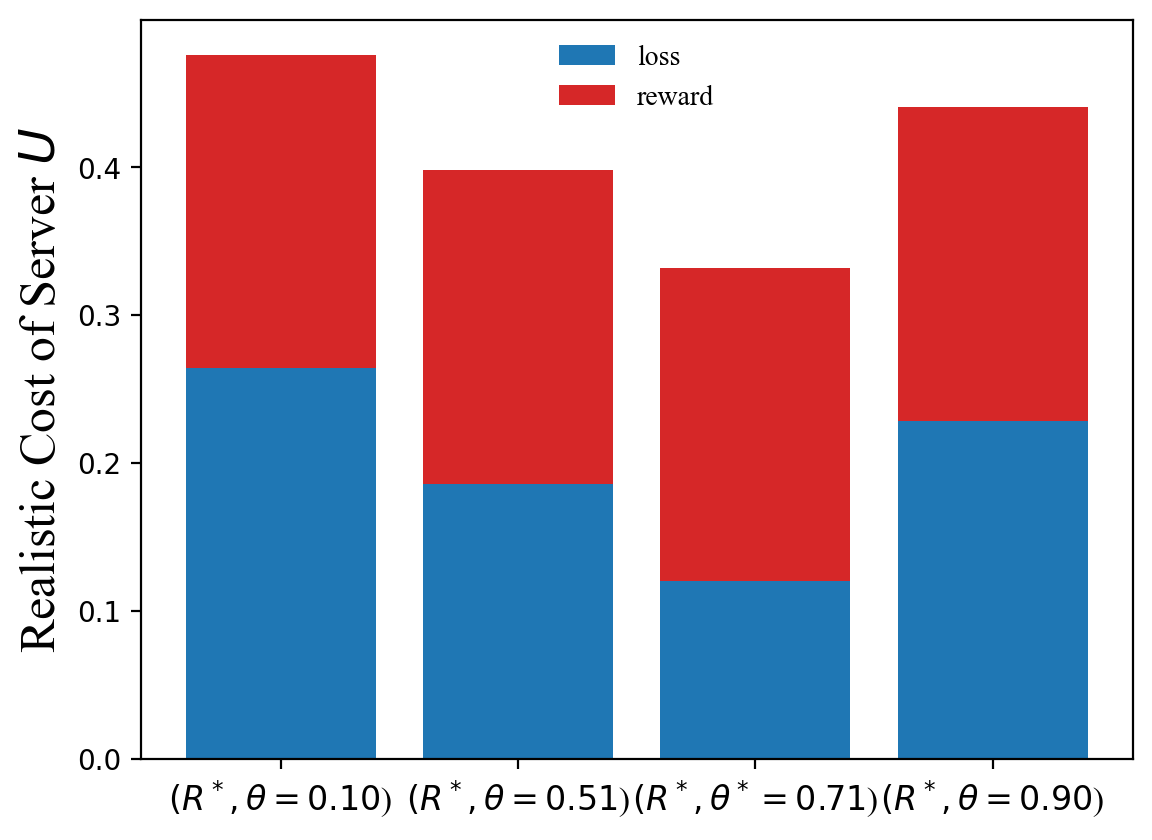
\includegraphics[width=\textwidth]{figures/figure_66_A.png}
%     \caption{$\sigma=0.1$}
% 	\end{subfigure}
%   \quad
% 	\begin{subfigure}{0.31\textwidth}
% 		\centering
% 		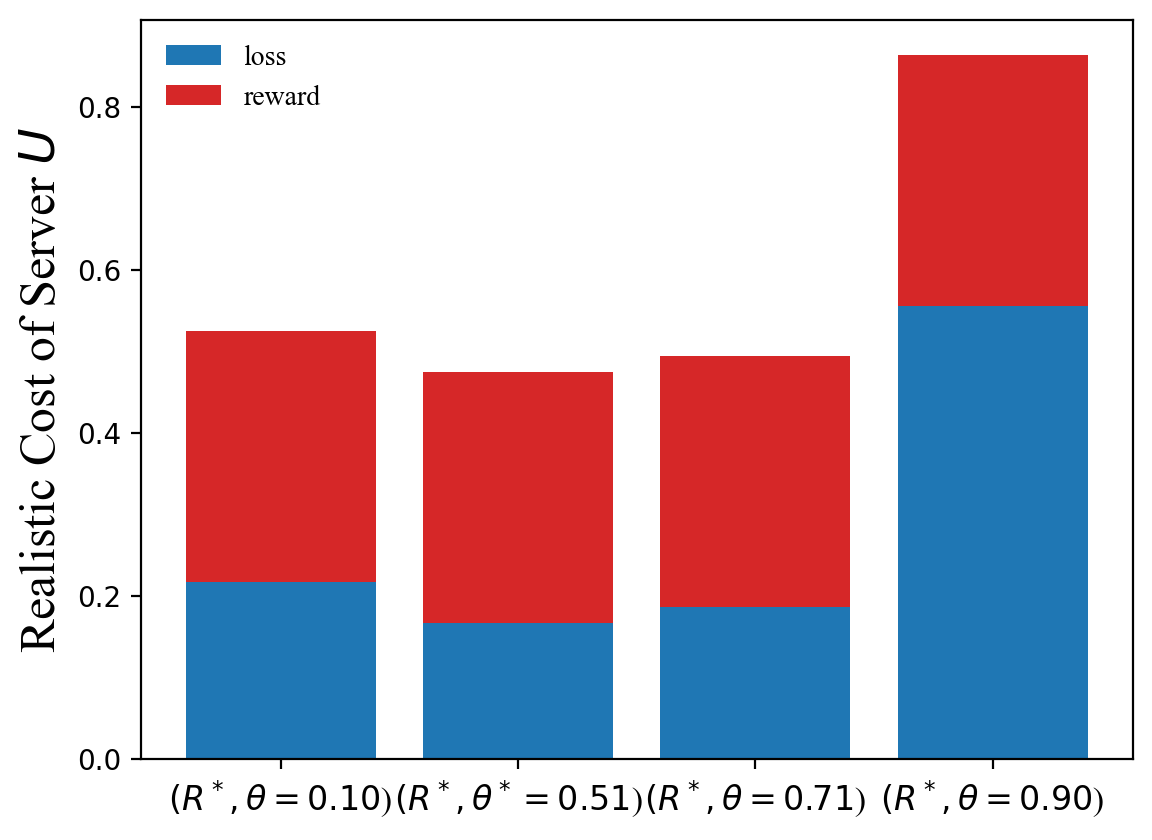
\includegraphics[width=\textwidth]{figures/figure_66_B.png}
%     \caption{$\sigma=0.3$}
% 	\end{subfigure}
%   \quad
%   \begin{subfigure}{0.31\textwidth}
% 		\centering
% 		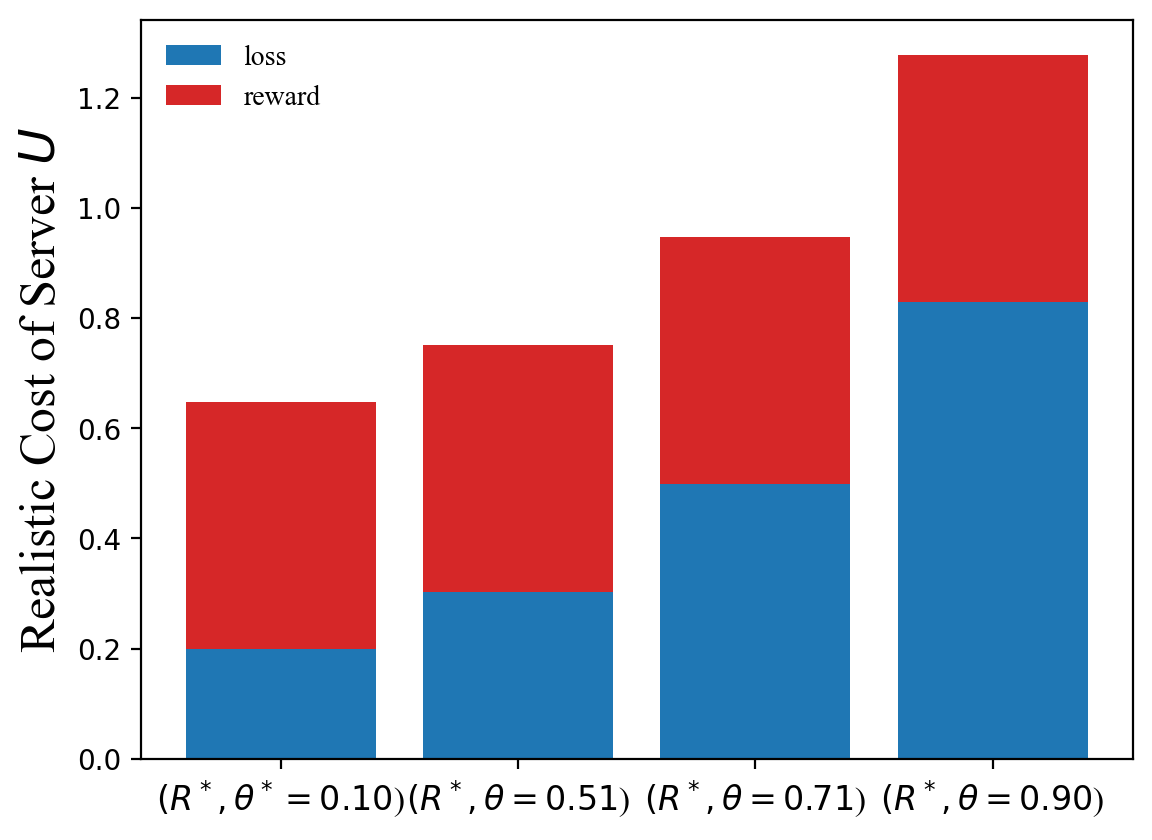
\includegraphics[width=\textwidth]{figures/figure_66_C.png}
%     \caption{$\sigma=0.7$}
% 	\end{subfigure}
% 	\caption{The effect of $\theta$ on cost}
% \end{figure*}

% \textit{Effect of initiative data on server' cost:}
% \begin{figure*}
% 	\begin{subfigure}{0.31\textwidth}
% 		\centering
%     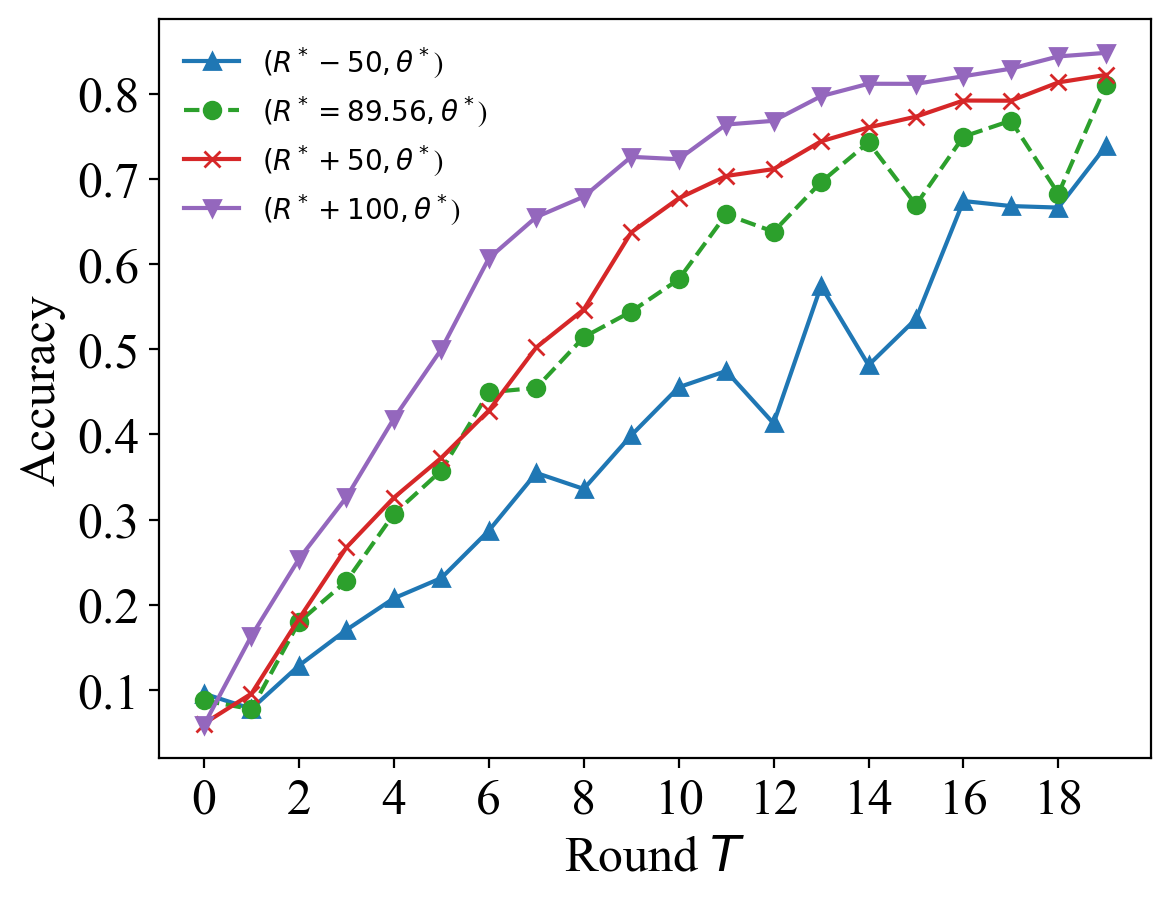
\includegraphics[width=\textwidth]{figures/figure_74_A.png}
%     \caption{$\sigma=0.1$}
% 	\end{subfigure}
%   \quad
% 	\begin{subfigure}{0.31\textwidth}
% 		\centering
% 		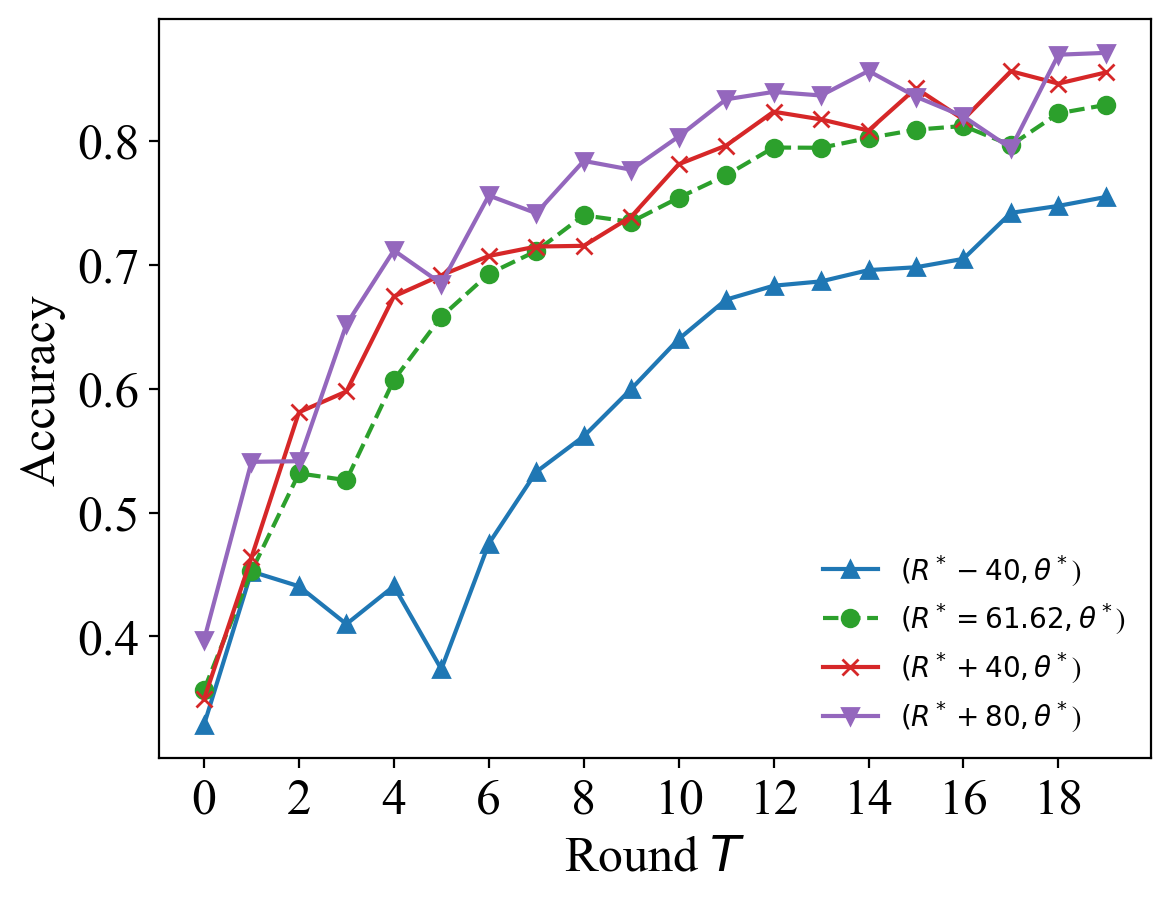
\includegraphics[width=\textwidth]{figures/figure_74_B.png}
%     \caption{$\sigma=0.3$}
% 	\end{subfigure}
%   \quad
%   \begin{subfigure}{0.31\textwidth}
% 		\centering
% 		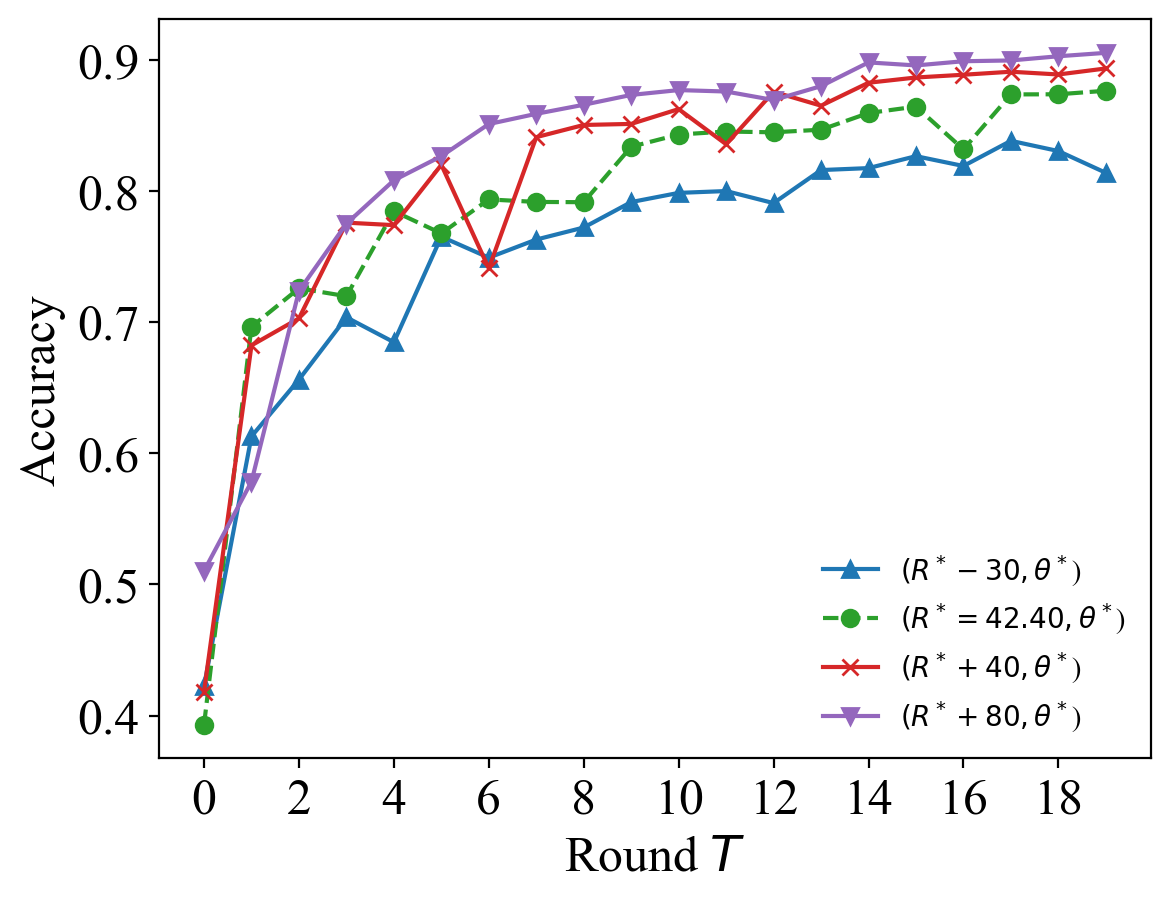
\includegraphics[width=\textwidth]{figures/figure_74_C.png}
%     \caption{$\sigma=0.7$}
% 	\end{subfigure}
% 	\caption{The effect of $R$ on model performance}
% \end{figure*}

% \textit{Effect of initiative data on server' cost:}
% \begin{figure*}
% 	\begin{subfigure}{0.31\textwidth}
% 		\centering
%     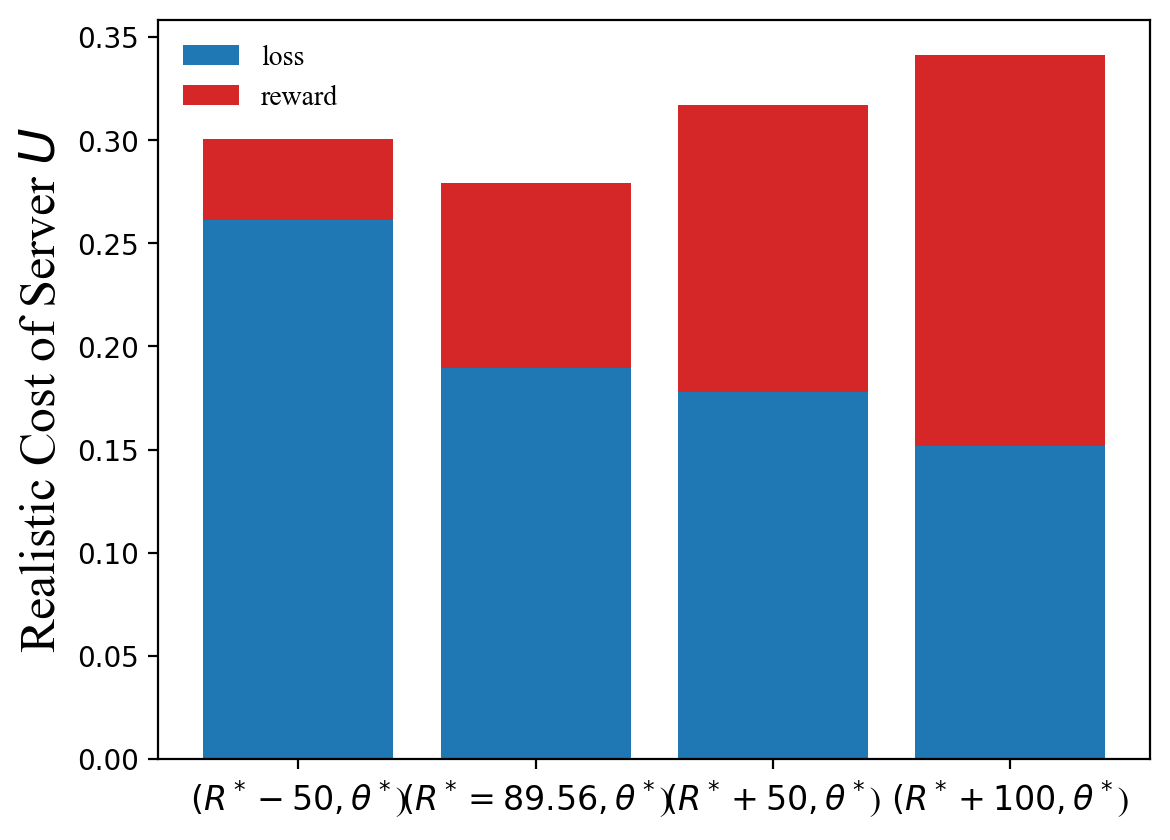
\includegraphics[width=\textwidth]{figures/figure_75_A.png}
%     \caption{$\sigma=0.1$}
% 	\end{subfigure}
%   \quad
% 	\begin{subfigure}{0.31\textwidth}
% 		\centering
% 		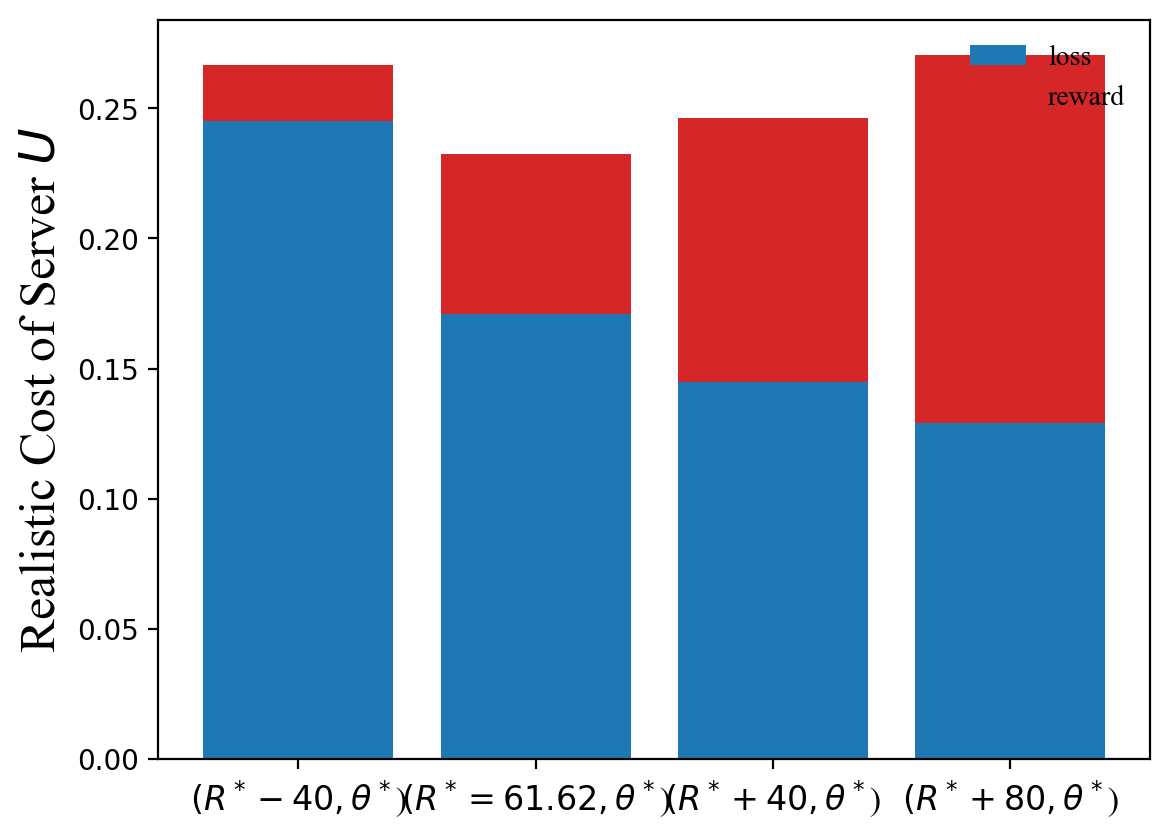
\includegraphics[width=\textwidth]{figures/figure_75_B.png}
%     \caption{$\sigma=0.3$}
% 	\end{subfigure}
%   \quad
%   \begin{subfigure}{0.31\textwidth}
% 		\centering
% 		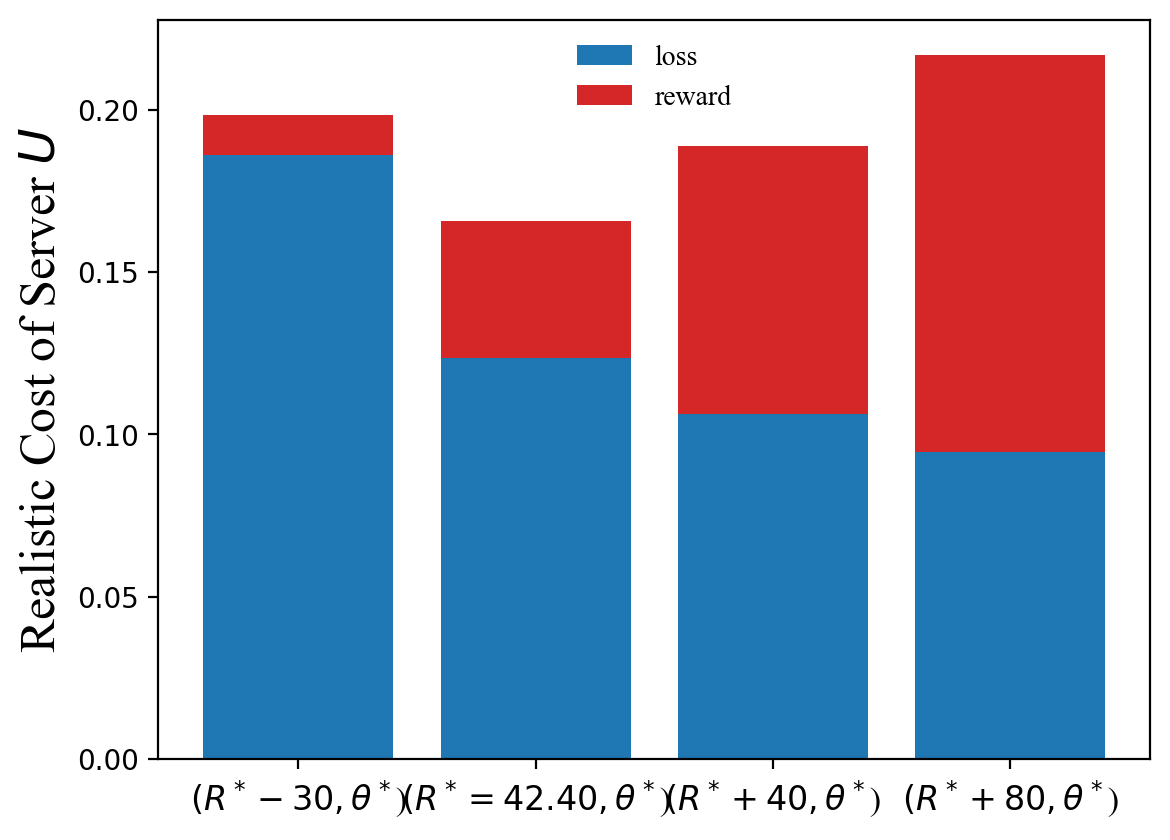
\includegraphics[width=\textwidth]{figures/figure_75_C.png}
%     \caption{$\sigma=0.7$}
% 	\end{subfigure}
% 	\caption{The effect of $R$ on cost}
% \end{figure*}

\textbf{Effect of Hyperparameters: }
In this paragraph, we explore the result of effect of hyperparameters such as time-sensitive coefficient $\sigma$ and initial volume of data $D(0)$ on exprements.

For generalization, we set three task modes: low time sensitivity, normal sensitivity and high sensitivity.
The low time sensitivity mode usually corresponds to weak-dynamic scenarios where the data distribution is stable, such as long-term agriculture analysis or chronic disease analysis, while the high time sensitivity mode corresponds to strong-dynamic scenarios where the data distribution is unstable, such as real-time personalized recommendation and smart transporation.  
To simulate the above three modes in the experiments, we set the time sensitivity coefficient of $\sigma$ as $0.1, 0.3$ and $0.7$ respectively.
The optimal strategies under various $\sigma$ are shown in Figure \ref{fig:hyperparam}. As $\sigma$ increases, the optimal reward $R$ rises with optimal conservation rate $\theta$ drops.
It matches the intution that when facing tasks with higher time sensitivity, the value of previous data decrease. Server need to guide clients to abandon previous data as well as to collect new data in time.
This illustrates that our proposed strategy can be applied in various different scenarios.

Next, we exhibite the effect of initial data size $D_k(0)$ on data volume.
There is a key question about \textit{whether the volume of data keeps dropping along with communication rounds}. It seems elusive from the perspective of intution.
For comparison, We sampe three initial data volume: $D^1(0)=50$, $D^2(0)=100$ and $D^3(0)=700$. 
The results is shown in Figure \ref{fig:hyperparam}. We can observe that $D(0)$ only makes differneces on a few rounds at the begining of training, then they converge to the same stationary state and drop synchronously.
From the aspect of mathematics, stationary state doesn't depend on $D(0)$ as demonstrated in remark \ref{remark:stationary state}. 
Therefore, the answer to the above question is that the trend of curve of data volumn banks on $D(0)$ and stationary state at the same time.
If $D(0)$ is greater than stationary state, then $D(t)$ keeps rising before reaching the stationary state, and vice versa.

\begin{figure}
	\begin{minipage}{0.49\linewidth}
		\centerline{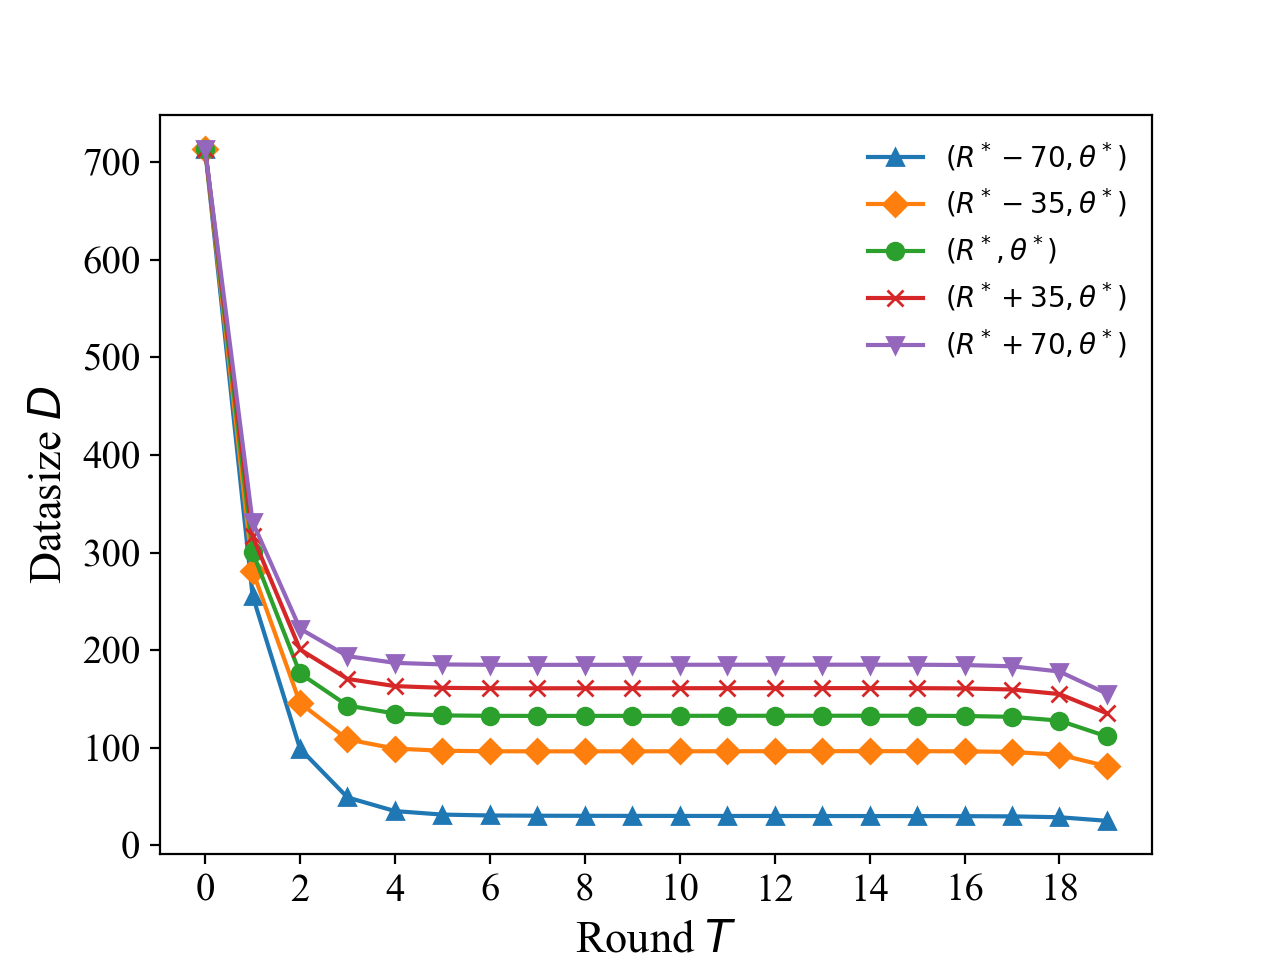
\includegraphics[width=\textwidth]{figures/figure_55_B.png}}
	\end{minipage}
	\begin{minipage}{0.49\linewidth}
		\centerline{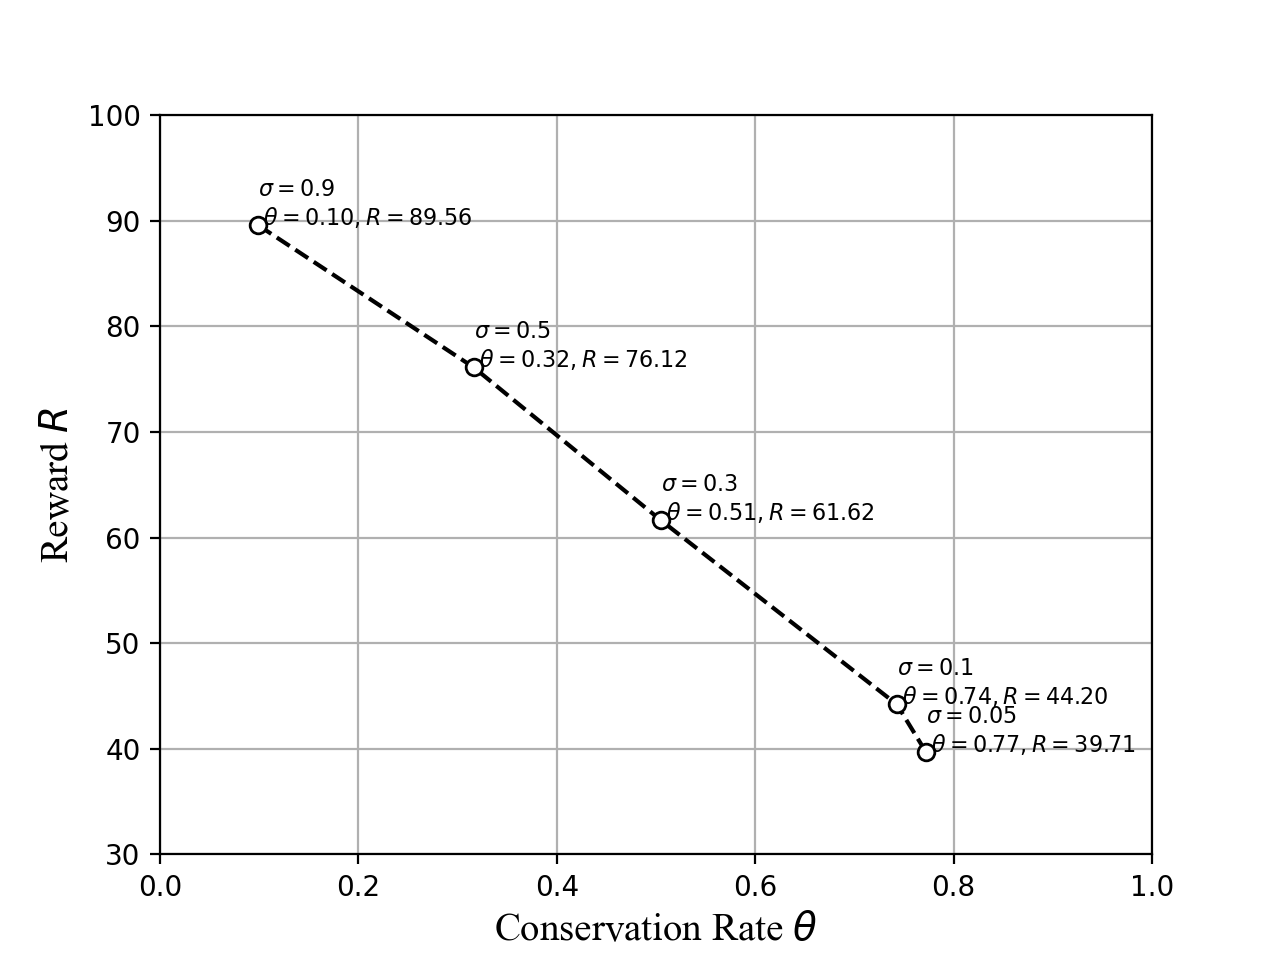
\includegraphics[width=\textwidth]{figures/figure_80.png}}
	\end{minipage}
	\caption{Comparative analysis of increment $\Delta_k(t)$ against a particular client $k$ versus communication rounds $t$ across various value of $\theta$ ranging from $0$ to $1$ (\textbf{left}) and $R$ ranging from $0$ to $100$ (\textbf{right}).}
  \label{fig:hyperparam}
\end{figure}

% \newpage
% \section{Electronic Submission}
% \label{submission}

% Submission to ICML 2025 will be entirely electronic, via a web site
% (not email). Information about the submission process and \LaTeX\ templates
% are available on the conference web site at:
% \begin{center}
% \textbf{\texttt{http://icml.cc/}}
% \end{center}

% The guidelines below will be enforced for initial submissions and
% camera-ready copies. Here is a brief summary:
% \begin{itemize}
% \item Submissions must be in PDF\@. 
% \item If your paper has appendices, submit the appendix together with the main body and the references \textbf{as a single file}. Reviewers will not look for appendices as a separate PDF file. So if you submit such an extra file, reviewers will very likely miss it.
% \item Page limit: The main body of the paper has to be fitted to 8 pages, excluding references and appendices; the space for the latter two is not limited in pages, but the total file size may not exceed 10MB. For the final version of the paper, authors can add one extra page to the main body.
% \item \textbf{Do not include author information or acknowledgements} in your
%     initial submission.
% \item Your paper should be in \textbf{10 point Times font}.
% \item Make sure your PDF file only uses Type-1 fonts.
% \item Place figure captions \emph{under} the figure (and omit titles from inside
%     the graphic file itself). Place table captions \emph{over} the table.
% \item References must include page numbers whenever possible and be as complete
%     as possible. Place multiple citations in chronological order.
% \item Do not alter the style template; in particular, do not compress the paper
%     format by reducing the vertical spaces.
% \item Keep your abstract brief and self-contained, one paragraph and roughly
%     4--6 sentences. Gross violations will require correction at the
%     camera-ready phase. The title should have content words capitalized.
% \end{itemize}

% \subsection{Submitting Papers}

% \textbf{Anonymous Submission:} ICML uses double-blind review: no identifying
% author information may appear on the title page or in the paper
% itself. \cref{author info} gives further details.

% \medskip

% Authors must provide their manuscripts in \textbf{PDF} format.
% Furthermore, please make sure that files contain only embedded Type-1 fonts
% (e.g.,~using the program \texttt{pdffonts} in linux or using
% File/DocumentProperties/Fonts in Acrobat). Other fonts (like Type-3)
% might come from graphics files imported into the document.

% Authors using \textbf{Word} must convert their document to PDF\@. Most
% of the latest versions of Word have the facility to do this
% automatically. Submissions will not be accepted in Word format or any
% format other than PDF\@. Really. We're not joking. Don't send Word.

% Those who use \textbf{\LaTeX} should avoid including Type-3 fonts.
% Those using \texttt{latex} and \texttt{dvips} may need the following
% two commands:

% {\footnotesize
% \begin{verbatim}
% dvips -Ppdf -tletter -G0 -o paper.ps paper.dvi
% ps2pdf paper.ps
% \end{verbatim}}
% It is a zero following the ``-G'', which tells dvips to use
% the config.pdf file. Newer \TeX\ distributions don't always need this
% option.

% Using \texttt{pdflatex} rather than \texttt{latex}, often gives better
% results. This program avoids the Type-3 font problem, and supports more
% advanced features in the \texttt{microtype} package.

% \textbf{Graphics files} should be a reasonable size, and included from
% an appropriate format. Use vector formats (.eps/.pdf) for plots,
% lossless bitmap formats (.png) for raster graphics with sharp lines, and
% jpeg for photo-like images.

% The style file uses the \texttt{hyperref} package to make clickable
% links in documents. If this causes problems for you, add
% \texttt{nohyperref} as one of the options to the \texttt{icml2025}
% usepackage statement.


% \subsection{Submitting Final Camera-Ready Copy}

% The final versions of papers accepted for publication should follow the
% same format and naming convention as initial submissions, except that
% author information (names and affiliations) should be given. See
% \cref{final author} for formatting instructions.

% The footnote, ``Preliminary work. Under review by the International
% Conference on Machine Learning (ICML). Do not distribute.'' must be
% modified to ``\textit{Proceedings of the
% $\mathit{42}^{nd}$ International Conference on Machine Learning},
% Vancouver, Canada, PMLR 267, 2025.
% Copyright 2025 by the author(s).''

% For those using the \textbf{\LaTeX} style file, this change (and others) is
% handled automatically by simply changing
% $\mathtt{\backslash usepackage\{icml2025\}}$ to
% $$\mathtt{\backslash usepackage[accepted]\{icml2025\}}$$
% Authors using \textbf{Word} must edit the
% footnote on the first page of the document themselves.

% Camera-ready copies should have the title of the paper as running head
% on each page except the first one. The running title consists of a
% single line centered above a horizontal rule which is $1$~point thick.
% The running head should be centered, bold and in $9$~point type. The
% rule should be $10$~points above the main text. For those using the
% \textbf{\LaTeX} style file, the original title is automatically set as running
% head using the \texttt{fancyhdr} package which is included in the ICML
% 2025 style file package. In case that the original title exceeds the
% size restrictions, a shorter form can be supplied by using

% \verb|\icmltitlerunning{...}|

% just before $\mathtt{\backslash begin\{document\}}$.
% Authors using \textbf{Word} must edit the header of the document themselves.





% \section{Format of the Paper}

% All submissions must follow the specified format.

% \subsection{Dimensions}




% The text of the paper should be formatted in two columns, with an
% overall width of 6.75~inches, height of 9.0~inches, and 0.25~inches
% between the columns. The left margin should be 0.75~inches and the top
% margin 1.0~inch (2.54~cm). The right and bottom margins will depend on
% whether you print on US letter or A4 paper, but all final versions
% must be produced for US letter size.
% Do not write anything on the margins.

% The paper body should be set in 10~point type with a vertical spacing
% of 11~points. Please use Times typeface throughout the text.

% \subsection{Title}

% The paper title should be set in 14~point bold type and centered
% between two horizontal rules that are 1~point thick, with 1.0~inch
% between the top rule and the top edge of the page. Capitalize the
% first letter of content words and put the rest of the title in lower
% case.

% \subsection{Author Information for Submission}
% \label{author info}

% ICML uses double-blind review, so author information must not appear. If
% you are using \LaTeX\/ and the \texttt{icml2025.sty} file, use
% \verb+\icmlauthor{...}+ to specify authors and \verb+\icmlaffiliation{...}+ to specify affiliations. (Read the TeX code used to produce this document for an example usage.) The author information
% will not be printed unless \texttt{accepted} is passed as an argument to the
% style file.
% Submissions that include the author information will not
% be reviewed.

% \subsubsection{Self-Citations}

% If you are citing published papers for which you are an author, refer
% to yourself in the third person. In particular, do not use phrases
% that reveal your identity (e.g., ``in previous work \cite{langley00}, we
% have shown \ldots'').

% Do not anonymize citations in the reference section. The only exception are manuscripts that are
% not yet published (e.g., under submission). If you choose to refer to
% such unpublished manuscripts \cite{anonymous}, anonymized copies have
% to be submitted
% as Supplementary Material via OpenReview\@. However, keep in mind that an ICML
% paper should be self contained and should contain sufficient detail
% for the reviewers to evaluate the work. In particular, reviewers are
% not required to look at the Supplementary Material when writing their
% review (they are not required to look at more than the first $8$ pages of the submitted document).

% \subsubsection{Camera-Ready Author Information}
% \label{final author}

% If a paper is accepted, a final camera-ready copy must be prepared.
% %
% For camera-ready papers, author information should start 0.3~inches below the
% bottom rule surrounding the title. The authors' names should appear in 10~point
% bold type, in a row, separated by white space, and centered. Author names should
% not be broken across lines. Unbolded superscripted numbers, starting 1, should
% be used to refer to affiliations.

% Affiliations should be numbered in the order of appearance. A single footnote
% block of text should be used to list all the affiliations. (Academic
% affiliations should list Department, University, City, State/Region, Country.
% Similarly for industrial affiliations.)

% Each distinct affiliations should be listed once. If an author has multiple
% affiliations, multiple superscripts should be placed after the name, separated
% by thin spaces. If the authors would like to highlight equal contribution by
% multiple first authors, those authors should have an asterisk placed after their
% name in superscript, and the term ``\textsuperscript{*}Equal contribution"
% should be placed in the footnote block ahead of the list of affiliations. A
% list of corresponding authors and their emails (in the format Full Name
% \textless{}email@domain.com\textgreater{}) can follow the list of affiliations.
% Ideally only one or two names should be listed.

% A sample file with author names is included in the ICML2025 style file
% package. Turn on the \texttt{[accepted]} option to the stylefile to
% see the names rendered. All of the guidelines above are implemented
% by the \LaTeX\ style file.

% \subsection{Abstract}

% The paper abstract should begin in the left column, 0.4~inches below the final
% address. The heading `Abstract' should be centered, bold, and in 11~point type.
% The abstract body should use 10~point type, with a vertical spacing of
% 11~points, and should be indented 0.25~inches more than normal on left-hand and
% right-hand margins. Insert 0.4~inches of blank space after the body. Keep your
% abstract brief and self-contained, limiting it to one paragraph and roughly 4--6
% sentences. Gross violations will require correction at the camera-ready phase.

% \subsection{Partitioning the Text}

% You should organize your paper into sections and paragraphs to help
% readers place a structure on the material and understand its
% contributions.

% \subsubsection{Sections and Subsections}

% Section headings should be numbered, flush left, and set in 11~pt bold
% type with the content words capitalized. Leave 0.25~inches of space
% before the heading and 0.15~inches after the heading.

% Similarly, subsection headings should be numbered, flush left, and set
% in 10~pt bold type with the content words capitalized. Leave
% 0.2~inches of space before the heading and 0.13~inches afterward.

% Finally, subsubsection headings should be numbered, flush left, and
% set in 10~pt small caps with the content words capitalized. Leave
% 0.18~inches of space before the heading and 0.1~inches after the
% heading.

% Please use no more than three levels of headings.

% \subsubsection{Paragraphs and Footnotes}

% Within each section or subsection, you should further partition the
% paper into paragraphs. Do not indent the first line of a given
% paragraph, but insert a blank line between succeeding ones.

% You can use footnotes\footnote{Footnotes
% should be complete sentences.} to provide readers with additional
% information about a topic without interrupting the flow of the paper.
% Indicate footnotes with a number in the text where the point is most
% relevant. Place the footnote in 9~point type at the bottom of the
% column in which it appears. Precede the first footnote in a column
% with a horizontal rule of 0.8~inches.\footnote{Multiple footnotes can
% appear in each column, in the same order as they appear in the text,
% but spread them across columns and pages if possible.}

% \begin{figure}[ht]
% \vskip 0.2in
% \begin{center}
% \centerline{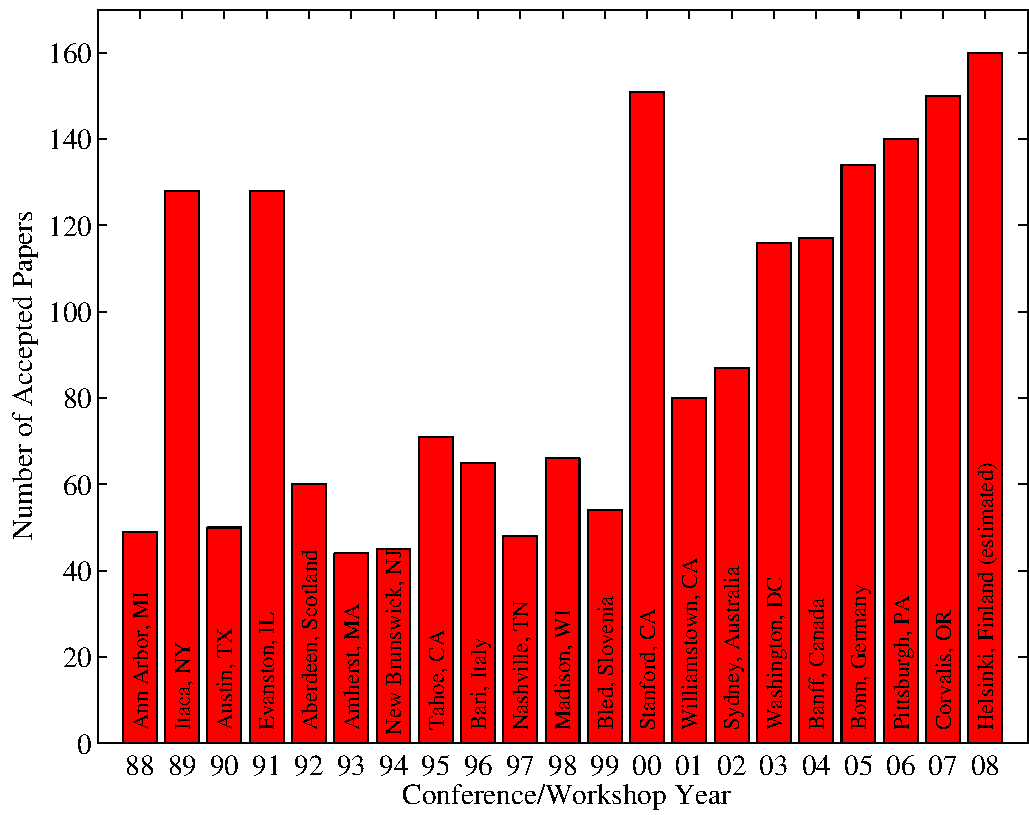
\includegraphics[width=\columnwidth]{icml_numpapers}}
% \caption{Historical locations and number of accepted papers for International
% Machine Learning Conferences (ICML 1993 -- ICML 2008) and International
% Workshops on Machine Learning (ML 1988 -- ML 1992). At the time this figure was
% produced, the number of accepted papers for ICML 2008 was unknown and instead
% estimated.}
% \label{icml-historical}
% \end{center}
% \vskip -0.2in
% \end{figure}

% \subsection{Figures}

% You may want to include figures in the paper to illustrate
% your approach and results. Such artwork should be centered,
% legible, and separated from the text. Lines should be dark and at
% least 0.5~points thick for purposes of reproduction, and text should
% not appear on a gray background.

% Label all distinct components of each figure. If the figure takes the
% form of a graph, then give a name for each axis and include a legend
% that briefly describes each curve. Do not include a title inside the
% figure; instead, the caption should serve this function.

% Number figures sequentially, placing the figure number and caption
% \emph{after} the graphics, with at least 0.1~inches of space before
% the caption and 0.1~inches after it, as in
% \cref{icml-historical}. The figure caption should be set in
% 9~point type and centered unless it runs two or more lines, in which
% case it should be flush left. You may float figures to the top or
% bottom of a column, and you may set wide figures across both columns
% (use the environment \texttt{figure*} in \LaTeX). Always place
% two-column figures at the top or bottom of the page.

% \subsection{Algorithms}

% If you are using \LaTeX, please use the ``algorithm'' and ``algorithmic''
% environments to format pseudocode. These require
% the corresponding stylefiles, algorithm.sty and
% algorithmic.sty, which are supplied with this package.
% \cref{alg:example} shows an example.

% \begin{algorithm}[tb]
%    \caption{Bubble Sort}
%    \label{alg:example}
% \begin{algorithmic}
%    \STATE {\bfseries Input:} data $x_i$, size $m$
%    \REPEAT
%    \STATE Initialize $noChange = true$.
%    \FOR{$i=1$ {\bfseries to} $m-1$}
%    \IF{$x_i > x_{i+1}$}
%    \STATE Swap $x_i$ and $x_{i+1}$
%    \STATE $noChange = false$
%    \ENDIF
%    \ENDFOR
%    \UNTIL{$noChange$ is $true$}
% \end{algorithmic}
% \end{algorithm}

% \subsection{Tables}

% You may also want to include tables that summarize material. Like
% figures, these should be centered, legible, and numbered consecutively.
% However, place the title \emph{above} the table with at least
% 0.1~inches of space before the title and the same after it, as in
% \cref{sample-table}. The table title should be set in 9~point
% type and centered unless it runs two or more lines, in which case it
% should be flush left.

% % Note use of \abovespace and \belowspace to get reasonable spacing
% % above and below tabular lines.

% \begin{table}[t]
% \caption{Classification accuracies for naive Bayes and flexible
% Bayes on various data sets.}
% \label{sample-table}
% \vskip 0.15in
% \begin{center}
% \begin{small}
% \begin{sc}
% \begin{tabular}{lcccr}
% \toprule
% Data set & Naive & Flexible & Better? \\
% \midrule
% Breast    & 95.9$\pm$ 0.2& 96.7$\pm$ 0.2& $\surd$ \\
% Cleveland & 83.3$\pm$ 0.6& 80.0$\pm$ 0.6& $\times$\\
% Glass2    & 61.9$\pm$ 1.4& 83.8$\pm$ 0.7& $\surd$ \\
% Credit    & 74.8$\pm$ 0.5& 78.3$\pm$ 0.6&         \\
% Horse     & 73.3$\pm$ 0.9& 69.7$\pm$ 1.0& $\times$\\
% Meta      & 67.1$\pm$ 0.6& 76.5$\pm$ 0.5& $\surd$ \\
% Pima      & 75.1$\pm$ 0.6& 73.9$\pm$ 0.5&         \\
% Vehicle   & 44.9$\pm$ 0.6& 61.5$\pm$ 0.4& $\surd$ \\
% \bottomrule
% \end{tabular}
% \end{sc}
% \end{small}
% \end{center}
% \vskip -0.1in
% \end{table}

% Tables contain textual material, whereas figures contain graphical material.
% Specify the contents of each row and column in the table's topmost
% row. Again, you may float tables to a column's top or bottom, and set
% wide tables across both columns. Place two-column tables at the
% top or bottom of the page.

% \subsection{Theorems and such}
% The preferred way is to number definitions, propositions, lemmas, etc. consecutively, within sections, as shown below.
% \begin{definition}
% \label{def:inj}
% A function $f:X \to Y$ is injective if for any $x,y\in X$ different, $f(x)\ne f(y)$.
% \end{definition}
% Using \cref{def:inj} we immediate get the following result:
% \begin{proposition}
% If $f$ is injective mapping a set $X$ to another set $Y$, 
% the cardinality of $Y$ is at least as large as that of $X$
% \end{proposition}
% \begin{proof} 
% Left as an exercise to the reader. 
% \end{proof}
% \cref{lem:usefullemma} stated next will prove to be useful.
% \begin{lemma}
% \label{lem:usefullemma}
% For any $f:X \to Y$ and $g:Y\to Z$ injective functions, $f \circ g$ is injective.
% \end{lemma}
% \begin{theorem}
% \label{thm:bigtheorem}
% If $f:X\to Y$ is bijective, the cardinality of $X$ and $Y$ are the same.
% \end{theorem}
% An easy corollary of \cref{thm:bigtheorem} is the following:
% \begin{corollary}
% If $f:X\to Y$ is bijective, 
% the cardinality of $X$ is at least as large as that of $Y$.
% \end{corollary}
% \begin{assumption}
% The set $X$ is finite.
% \label{ass:xfinite}
% \end{assumption}
% \begin{remark}
% According to some, it is only the finite case (cf. \cref{ass:xfinite}) that is interesting.
% \end{remark}
% %restatable

% \subsection{Citations and References}

% Please use APA reference format regardless of your formatter
% or word processor. If you rely on the \LaTeX\/ bibliographic
% facility, use \texttt{natbib.sty} and \texttt{icml2025.bst}
% included in the style-file package to obtain this format.

% Citations within the text should include the authors' last names and
% year. If the authors' names are included in the sentence, place only
% the year in parentheses, for example when referencing Arthur Samuel's
% pioneering work \yrcite{Samuel59}. Otherwise place the entire
% reference in parentheses with the authors and year separated by a
% comma \cite{Samuel59}. List multiple references separated by
% semicolons \cite{kearns89,Samuel59,mitchell80}. Use the `et~al.'
% construct only for citations with three or more authors or after
% listing all authors to a publication in an earlier reference \cite{MachineLearningI}.

% Authors should cite their own work in the third person
% in the initial version of their paper submitted for blind review.
% Please refer to \cref{author info} for detailed instructions on how to
% cite your own papers.

% Use an unnumbered first-level section heading for the references, and use a
% hanging indent style, with the first line of the reference flush against the
% left margin and subsequent lines indented by 10 points. The references at the
% end of this document give examples for journal articles \cite{Samuel59},
% conference publications \cite{langley00}, book chapters \cite{Newell81}, books
% \cite{DudaHart2nd}, edited volumes \cite{MachineLearningI}, technical reports
% \cite{mitchell80}, and dissertations \cite{kearns89}.

% Alphabetize references by the surnames of the first authors, with
% single author entries preceding multiple author entries. Order
% references for the same authors by year of publication, with the
% earliest first. Make sure that each reference includes all relevant
% information (e.g., page numbers).

% Please put some effort into making references complete, presentable, and
% consistent, e.g. use the actual current name of authors.
% If using bibtex, please protect capital letters of names and
% abbreviations in titles, for example, use \{B\}ayesian or \{L\}ipschitz
% in your .bib file.

% \section*{Accessibility}
% Authors are kindly asked to make their submissions as accessible as possible for everyone including people with disabilities and sensory or neurological differences.
% Tips of how to achieve this and what to pay attention to will be provided on the conference website \url{http://icml.cc/}.

% \section*{Software and Data}

% If a paper is accepted, we strongly encourage the publication of software and data with the
% camera-ready version of the paper whenever appropriate. This can be
% done by including a URL in the camera-ready copy. However, \textbf{do not}
% include URLs that reveal your institution or identity in your
% submission for review. Instead, provide an anonymous URL or upload
% the material as ``Supplementary Material'' into the OpenReview reviewing
% system. Note that reviewers are not required to look at this material
% when writing their review.

% % Acknowledgements should only appear in the accepted version.
% \section*{Acknowledgements}

% \textbf{Do not} include acknowledgements in the initial version of
% the paper submitted for blind review.

% If a paper is accepted, the final camera-ready version can (and
% usually should) include acknowledgements.  Such acknowledgements
% should be placed at the end of the section, in an unnumbered section
% that does not count towards the paper page limit. Typically, this will 
% include thanks to reviewers who gave useful comments, to colleagues 
% who contributed to the ideas, and to funding agencies and corporate 
% sponsors that provided financial support.

% \section*{Impact Statement}

% Authors are \textbf{required} to include a statement of the potential 
% broader impact of their work, including its ethical aspects and future 
% societal consequences. This statement should be in an unnumbered 
% section at the end of the paper (co-located with Acknowledgements -- 
% the two may appear in either order, but both must be before References), 
% and does not count toward the paper page limit. In many cases, where 
% the ethical impacts and expected societal implications are those that 
% are well established when advancing the field of Machine Learning, 
% substantial discussion is not required, and a simple statement such 
% as the following will suffice:

% ``This paper presents work whose goal is to advance the field of 
% Machine Learning. There are many potential societal consequences 
% of our work, none which we feel must be specifically highlighted here.''

% The above statement can be used verbatim in such cases, but we 
% encourage authors to think about whether there is content which does 
% warrant further discussion, as this statement will be apparent if the 
% paper is later flagged for ethics review.


% In the unusual situation where you want a paper to appear in the
% references without citing it in the main text, use \nocite
\nocite{langley00}

\bibliography{example_paper}
\bibliographystyle{icml2025}


%%%%%%%%%%%%%%%%%%%%%%%%%%%%%%%%%%%%%%%%%%%%%%%%%%%%%%%%%%%%%%%%%%%%%%%%%%%%%%%
%%%%%%%%%%%%%%%%%%%%%%%%%%%%%%%%%%%%%%%%%%%%%%%%%%%%%%%%%%%%%%%%%%%%%%%%%%%%%%%
% APPENDIX
%%%%%%%%%%%%%%%%%%%%%%%%%%%%%%%%%%%%%%%%%%%%%%%%%%%%%%%%%%%%%%%%%%%%%%%%%%%%%%%
%%%%%%%%%%%%%%%%%%%%%%%%%%%%%%%%%%%%%%%%%%%%%%%%%%%%%%%%%%%%%%%%%%%%%%%%%%%%%%%
\newpage
\appendix
\onecolumn
In the appendix, the complete proofs of theoretic results provided in the main text and more contents about experiment will be exhibited in detail.
\section{Proof of Theoretic Results}
\subsection{Proof of Remark \ref{remark:generalformula}}
\label{proof:generalformula}
\begin{proof}
    According to the definition of DoS, we have
    \begin{align}
      S_k(t+1) & = S_k(t) \frac{\theta D_k(t)}{D_k(t+1)} + 1 = S_k(t)\left(1 - \frac{\Delta_k(t)}{D_k(t+1)}\right) + 1 \notag \\
               & = \left(S_k(t-1) \frac{\theta D_k(t-1)}{D_k(t)} + 1\right) \frac{\theta D_k(t)}{D_k(t+1)} + 1 \notag \\
               & = S_k(t-1) \frac{\theta^2 D_k(t-1)}{D_k(t+1)} + \frac{\theta D_k(t)}{D_k(t+1)} + 1 \notag \\
               & = S_k(t-2) \frac{\theta^3 D_k(t-2)}{D_k(t+1)} + \frac{\theta^2 D_k(t-1)}{D_k(t+1)} + \frac{\theta D_k(t)}{D_k(t+1)} + 1 \notag \\
               & = \cdots \notag \\
               & = S_k(0) \frac{\theta^{t+1} D_k(0)}{D_k(t+1)} + \frac{\theta^t D_k(1)}{D_k(t+1)} + \cdots + \frac{\theta^2 D_k(t-1)}{D_k(t+1)} + \frac{\theta D_k(t)}{D_k(t+1)} + 1 \notag \\
               & = \sum_{\tau = 0}^{t+1} \frac{\theta^{t+1-\tau} D_k(\tau)}{D_k(t+1)}.
    \end{align}
  \end{proof}

\subsection{Proof of Theorem \ref{theorem:upperbound}}
\begin{proof}
  \label{proof:upperbound}
  Let's pay attention to the round $t+1$.
  \begin{align}
    \label{proof:init}
      & E[F(w(t+1)|D(t+1))-F(w(t)|D(t))] \notag \\
      = & E[F(w(t+1)|D(t))-F(w(t)|D(t))] + E[F(w(t+1)|D(t+1))-F(w(t+1)|D(t))] \notag \\
      = & \underbrace{E[F(w(t+1)|D(t))-F(w(t)|D(t))]}_A + \Omega_t,
  \end{align}
  where $\Omega_t = E[F(w(t+1)|D(t+1))-F(w(t+1)|D(t))]$. It captures the expected difference of global loss function based on the same global model $w(t)$ between buffered data at present round $D(t)$ and at previous round $D(t - 1)$. 
  Then we focus on $A$. Since $F_k(w)$ is $\beta$-Lipschitz smooth, we have
  \begin{align}
    \label{proof:boundA}
        & E[F(w(t+1)|D(t))-F(w(t)|D(t))] \notag \\
    \leq & E\left\langle \nabla F(w(t)|D(t)), w(t+1)-w(t)|D(t)\right\rangle + \frac{\beta}{2}E{\Vert w(t+1)-w(t)|D(t) \Vert}^2 \notag \\
    =    & E\left\langle \nabla F(w(t)|D(t)), (-\eta)\nabla F(w(t)|D(t))\right\rangle + \frac{\beta}{2}E{\Vert w(t+1)-w(t)|D(t) \Vert}^2 \notag \\ 
    =    & (-\eta) \Vert \nabla F(w(t)|D(t))\Vert^2 + \underbrace{\frac{\beta}{2}E{\Vert w(t+1)-w(t)|D(t) \Vert}^2}_{B}.
  \end{align}
  Next, we focus on bounding $B$. Because the stochastic gradient of $\nabla F_k(w)$ is unbiased and variance-bounded, we have 
  \begin{align}
    \label{proof:boundB}
         & \frac{\beta}{2} E {\Vert w(t+1) - w(t) | D(t) \Vert}^2 \notag \\
    =    & \frac{\beta}{2} E {\Vert (-\eta) \nabla F(w(t)|D(t))\Vert}^2 \notag \\
    \leq & \beta\eta^2 E{\Vert\nabla F(w(t)|D(t))\Vert}^2 \notag \\
    =    & \beta\eta^2 E{\left\Vert \sum_{k=1}^{N} \frac{D_k(t)}{D(t)} \nabla F_k(w(t)|D_k(t))\right\Vert}^2 \notag \\
    \leq & \beta\eta^2 \sum_{k=1}^{N} \frac{D_k(t)}{D(t)} E\Vert\nabla F_k(w(t)|D_k(t))\Vert^2 \notag \\
    \leq & \beta\eta^2 \sum_{k=1}^{N} \frac{D_k(t)}{D(t)} \left(2\Vert\nabla F(w(t)|D(t))\Vert^2 + \frac{\psi^2}{D_k(t)} + S_k(t)\sigma^2\right) \notag \\
    =    & 2\beta\eta^2 \Vert\nabla F(w(t)|D(t))\Vert^2 + \beta\eta^2 \frac{N\psi^2}{D(t)} + \beta\eta^2 \sum_{k=1}^{N} \frac{D_k(t)}{D(t)} S_k(t) \sigma^2.
  \end{align}
  Substituting (\ref{proof:boundB}) into (\ref{proof:boundA}), we have
  \begin{align}
    \label{proof:substituteB}
    & E[F(w(t+1)|D(t)) - F(w(t)|D(t))] \notag \\
    \leq & \underbrace{ (2\beta \eta^2 - \eta) E{\Vert\nabla F(w(t)|D(t))\Vert}^2}_{C} + 2\beta\eta^2 \frac{N\psi^2}{D(t)} + \beta\eta^2 \sum_{k=1}^{N} \frac{D_k(t)}{D(t)} S_k(t) \sigma^2.
  \end{align}
  Now we bound $C$. We set $\eta < \frac{1}{2\beta}$, then $2\beta\eta^2 - \eta < 0$. Polyak Lojasiewicz condition holds for $F_k(w)$ due to strong convexity in assumptions:
  \begin{equation}
    E[F(w(t)|D(t))-F(w^*)] \leq \frac{1}{2\mu}E{\Vert\nabla F(w(t)|D(t))\Vert}_2^2.
  \end{equation}
  Thus the follwing inequality holds:
  \begin{equation}
    \label{proof:boundC}
    2\mu (2\beta\eta^2 - \eta)E[(F(w(t)|D(t))-F(w^*))] \geq (2\beta \eta^2 - \eta) E{\Vert\nabla F(w(t)|D(t))\Vert}_2^2.
  \end{equation}
  Substituting (\ref{proof:boundC}) into (\ref{proof:substituteB}), we have
  \begin{align}
    \label{proof:substituteC}
         & E[F(w(t+1)|D(t)) - F(w(t)|D(t))] \notag \\
    \leq & 2 \mu(2\beta\eta^2-\eta)E[F(w(t)|D(t))-F(w^*)] + 2\beta\eta^2 \frac{N\psi^2}{D(t)} + \beta\eta^2 \sum_{k=1}^{N} \frac{D_k(t)}{D(t)} S_k(t) \sigma^2.
  \end{align}
  Consequently, substituting (\ref{proof:substituteC}) into (\ref{proof:init}), we have
  \begin{align}
         & E[F(w(t+1)|D(t+1))-F(w(t)|D(t))] \notag \\
    =    & E[F(w(t+1)|D(t))-F(w(t)|D(t))] + \Omega_t \notag \\
    \leq & 2 \mu(2\beta\eta^2-\eta)E[F(w(t-1)|D(t))-F(w^*|D(t))] + 2\beta\eta^2 \frac{N\psi^2}{D(t)} + \beta\eta^2 \sum_{k=1}^{N} \frac{D_k(t)}{D(t)} S_k(t) \sigma^2 + \Omega_t.
  \end{align}
  Adding $E[F(w(t)|D(t))-F(w^*)]$ on both sides, we get
  \begin{align}
    \label{proof:preend}
         & E[F(w(t+1)|D(t+1)) - F(w^*)] \notag \\
    \leq & (1+4\mu\beta\eta^2-2\mu\eta)E[F(w(t)|D(t))-F(w^*)] + 2\beta\eta^2 \frac{N\psi^2}{D(t)} + \beta\eta^2 \sum_{k=1}^{N} \frac{D_k(t)}{D(t)} S_k(t) \sigma^2 + \Omega_t.
  \end{align}
  Then call (\ref{proof:preend}) recursively, we have
  \begin{align}
         & E[F(w(t+1)|D(t+1)) - F(w^*)] \notag \\
    \leq & (1+4\mu\beta\eta^2-2\mu\eta)E[F(w(t)|D(t))-F(w^*)] + 2\beta\eta^2 \frac{N\psi^2}{D(t)} + \beta\eta^2 \sum_{k=1}^{N} \frac{D_k(t)}{D(t)} S_k(t) \sigma^2 + \Omega_t \notag \\
    \leq & (1+4\mu\beta\eta^2-2\mu\eta)^2E[F(w(t-1)|D(t-1))-F(w^*)] \notag \\
         & + (1+4\mu\beta\eta^2-2\mu\eta)\left[2\beta\eta^2 \frac{N\psi^2}{D(t-1)} + \beta\eta^2 \sum_{k=1}^{N} \frac{D_k(t-1)}{D(t-1)} S_k(t-1) \sigma^2 + \Omega_{t-1}\right] \notag \\
         & + \left[2\beta\eta^2 \frac{N\psi^2}{D(t)} + \beta\eta^2 \sum_{k=1}^{N} \frac{D_k(t)}{D(t)} S_k(t) \sigma^2 + \Omega_t \right] \notag \\
    \leq & \cdots \notag \\
    \leq & (1+4\mu\beta\eta^2-2\mu\eta)^{t+1}E[F(w(0)|D(0))-F(w^*)] \notag \\
         & + \sum_{r=0}^t(1+4\mu\beta\eta^2-2\mu\eta)^r \left[2\beta\eta^2 \frac{N\psi^2}{D(t-r)} + \beta\eta^2 \sum_{k=1}^{N} \frac{D_k(t-r)}{D(t-r)} S_k(t-r) \sigma^2 + \Omega_{t-r} \right].
  \end{align}
  For ease of representation, let $\kappa_1 = 1 + 4\mu\beta\eta^2 - 2\mu\eta$, $\kappa_2 = 2\beta\eta^2$ and $\kappa_3 = \beta\eta^2$.
  Thus, the convergence upper bound after $T+1$ rounds can be reformulated as
  \begin{align}
         & E[F(w(T+1)|D(T+1)) - F(w^*)] \notag \\
    \leq & \kappa_1^{T+1} E[F(w(0)|D(0))-F(w^*)] + \sum_{t=0}^T\kappa_1^t \left[\kappa_2 \frac{N\psi^2}{D(T-t)} + \kappa_3 \sum_{k=1}^{N} \frac{D_k(T-t)}{D(T-t)} S_k(T-t) \sigma^2 + \Omega_{T-t} \right] \notag \\
    =    & \kappa_1^{T+1} E[F(w(0)|D(0))-F(w^*)] + \sum_{t=0}^{T}\kappa_1^{T-t} \left[\kappa_2 \frac{N\psi^2}{D(t)} + \kappa_3 \sum_{k=1}^{N} \frac{D_k(t)}{D(t)} S_k(t) \sigma^2 + \Omega_{t}\right].
  \end{align}
  Further, the convergence upper bound after $T$ rounds is
  \begin{align}
      & E[F(w(T)|D(T)) - F(w^*)] \notag \\ 
    = & \kappa_1^{T} E[F(w(0)|D(0))-F(w^*)] + \sum_{t=0}^{T-1}\kappa_1^{T-1-t} \left[\kappa_2 \frac{N\psi^2}{D(t)} + \kappa_3 \sum_{k=1}^{N} \frac{D_k(t)}{D(t)} S_k(t) \sigma^2 + \Omega_{t}\right].
  \end{align}
\end{proof}

\subsection{Proof of Proposition \ref{proposition:clientoptimalstrategy}}
\begin{proof}
    \label{proof:clientoptimalstrategy}
    For the long term optimization problem with dynamic constraint in (\ref{formulation:reformulated}), we construct a Hamilton equation $H_k(t)$ as follows:
    \begin{equation}
      H_k(t) = \frac{\overline{\delta_k}^{-1}D_k(t)}{\phi(t)}R - \alpha_k {\Delta_k(t)}^2 - \beta_k {D_k(t)^2} + \lambda_k(t+1)\left((\theta-1) D_k(t) + \Delta_k(t)\right).
    \end{equation}
    In addtion, $\frac{\partial^2 H_k(t)}{\partial {\Delta_k(t)}^2} = -2\alpha_k < 0$. That is, $H_k(t)$ is a concave function in $\Delta_k(t)$.
    To derive the optimal increment $\Delta_k(t)$ that minimize (\ref{formulation:reformulated}), it satisfies 
    \begin{align}
      \frac{\partial H_k(t)}{\partial \Delta_k(t)} & = 0, \\
      \frac{\partial H_k(t)}{\partial D_k(t)} & = \lambda_k(t) - \lambda_k(t+1).
    \end{align}
    By solving the above two formulas, we have
    \begin{align}
      \label{formulation:proof_delta}
      \Delta_k(t) & = \frac{1}{2\alpha_k} \lambda_k(t+1), \\
      \label{formulation:proof_lambda}
      \lambda_k(t) & = \theta \lambda_k(t+1) + \frac{\overline{\delta_k}^{-1}R}{\phi(t)} - 2\beta_k D_k(t).
    \end{align}  
    In addition, it can be derived that $\Delta_k(T-1) = 0$ because $\Delta_k(T-1)$ decides round $T$'s increment for client $k$.
    The buffered data volume $D_k(T)$ will not be involved in the training rounds which ranges from 0 to $T-1$.
    Therefore $D_k(T)$ cannot bring any benefit for client $k$ under high collection expenditure.
    It's feasible for client $k$ to set $\Delta_k(T-1) = 0$ and stop data collection.
    Based on this, the boundary condition can be expressed as
    \begin{align}
      \label{formulation:boundary}
      \lambda_k(T-1) & = \frac{\partial \left(\frac{\overline{\delta_k}^{-1}D(T-1)}{\phi(T-1)} R - \beta_k{D_k(T-1)}^2 \right)}{\partial D_k(T-1)} \notag \\
                     & = \frac{\overline{\delta_k}^{-1}R}{\phi(T-1)}- 2\beta_k D_k(T-1).
    \end{align}
    Combing (\ref{formulation:proof_lambda}) with (\ref{formulation:boundary}), we have
    \begin{align}
      \lambda_k(t) & = \theta \lambda_k(t+1) + \frac{\overline{\delta_k}^{-1}R}{\phi(t)} - 2\beta_k D_k(t) \notag \\
                  & = \theta^2 \lambda_k(t+2) + \theta\left(\frac{\overline{\delta_k}^{-1}R}{\phi(t+1)} - 2\beta_kD_k(t+1)\right) + \frac{\overline{\delta_k}^{-1}R}{\phi(t)} - 2\beta_kD_k(t) \notag \\
                  & = \cdots \notag \\
                  & = \theta^{T-1-t} \lambda_k(T-1) + \sum_{\tau=0}^{T-2-t} \theta^{\tau} \left(\frac{\overline{\delta_k}^{-1}R}{\phi(t + \tau)} - 2\beta_kD_k(t + \tau)\right) \notag \\
                  & = \theta^{T-1-t} \left(\frac{\overline{\delta_k}^{-1}R}{\phi(T-1)} - 2\beta_k D_k(T-1)\right) + \sum_{\tau=0}^{T-2-t} \theta^{\tau} \left(\frac{\overline{\delta_k}^{-1}R}{\phi(t + \tau)} - 2\beta_k D_k(t + \tau)\right) \notag \\
                  & = \sum_{\tau = 0}^{T - 1 - t} \theta^{\tau} \left(\frac{\overline{\delta_k}^{-1}R}{\phi(t + \tau)} - 2\beta_k D(t + \tau)\right) \notag \\
                  & = \sum_{\tau = t}^{T - 1} \theta^{\tau - t} \left(\frac{\overline{\delta_k}^{-1}R}{\phi(\tau)} - 2\beta_k D_k(\tau)\right).
    \end{align}
    and 
    \begin{align}
      \label{formulation:ready_lambda}
      \lambda_k(t+1) = \sum_{\tau = t + 1}^{T - 1} \theta^{\tau - t - 1} \left(\frac{\overline{\delta_k}^{-1}R}{\phi(\tau)} - 2\beta_k D_k(\tau)\right).
    \end{align}
    Substituting (\ref{formulation:ready_lambda}) into (\ref{formulation:proof_delta}), we obtain
    \begin{align}
      \label{formulation:ready_delta}
      \Delta_k(t) = \frac{1}{2 \alpha_k} \sum_{\tau = t + 1}^{T - 1} \theta^{\tau - t - 1} \left(\frac{\overline{\delta_k}^{-1}R}{\phi(\tau)} - 2\beta_k D_k(\tau)\right).
    \end{align}
    Substituting (\ref{formulation:ready_delta}) into (\ref{formulation:update}), we obtain
    \begin{align}
      D_k(t+1) & = \theta D_k(t) + \Delta_k(t) \notag \\
            & = \theta^2 D_k(t-1) + \theta \Delta_k(t-1) + \Delta_k(t) \notag \\
            & = \cdots \notag \\
            & = \theta^{t+1} D_k(0) + \sum_{\tau = 0}^{t} \theta^{t-\tau} \Delta_k(\tau).
    \end{align}
    with $t \in [0, T-2]$ and $\Delta_k(T-1) = 0$.
  \end{proof}

\subsection{Proof of Remark \ref{remark:stationary state}}
\begin{proof}
  \label{proof:stationary state}
  Under the infinite time horizon $T \rightarrow \infty$, the optimal strategy of a particular client $k$ in (\ref{formulation:delta}) is
  \begin{align}
    \Delta_k(t) & = \frac{1}{2\alpha_k} \sum_{\tau = t + 1}^{\infty} \theta^{\tau - t - 1} \left(\frac{R}{\phi(\tau)} - 2\beta_k D_k(\tau)\right) \\
                & = \frac{1}{2\alpha_k} \left[\left(\frac{R}{\phi(t+1)} - 2\beta_kD_k(t+1)\right) + \theta\left(\frac{R}{\phi(t+2)} - 2\beta_kD_k(t+2)\right) + \cdots + \theta^\infty\left(\frac{R}{\phi(\infty)}-2\beta_kD_k(\infty)\right)\right], 
  \end{align}
  Thereby, when $t$ trends to $\infty$, the optimal strategy is as follows:
  \begin{align}
    \lim_{t\rightarrow\infty} \Delta_k(t) & = \frac{1}{2\alpha_k} \left[\left(\frac{R}{\phi(\infty))} - 2\beta_kD_k(\infty)\right) + \theta\left(\frac{R}{\phi(\infty)} - 2\beta_kD_k(\infty)\right) + \cdots + \theta^\infty\left(\frac{R}{\phi(\infty)}-2\beta_kD_k(\infty)\right)\right] \\
    & = \frac{1}{2\alpha_k(1-\theta)} \left(\frac{R}{\phi(\infty)} - 2\beta_kD_k(\infty)\right).
  \end{align}  
  
\end{proof}

\subsection{Proof of Proposition \ref{proposition:fixed point}}
\begin{proof}
  \label{proof:fixed_point}
  According to Brouwer's fixed point theorem, we need to prove that $\Psi$ is a continuous mapping from a closed set to itself.
  First, we prove that $\Psi$ is a mapping from a close set to itself.
  We bound $D_k(t)$ as [0, U], where $D_k(t) \geq 0$ means buffered data volume must be non-negative, and $D_k(t) \leq U$ means the storage capacity of buffer can't exceed $U$.
  Then, the domain of $\Psi$ can be bounded as
  \begin{equation}
    \Pi = [0, U] \times [0, U] \times \cdots \times [0, U].
  \end{equation}
  Therefore, $\Psi$ is a mapping from a close set $\Pi$ to itself.
  
  Then, we prove that $\Psi$ is a continuous mapping in $\Pi$.
  It's obvious that $\Psi_k(t)$ is continuous because $D_k(t)$ is continuous.
  $\Psi$ is a linear combination of $\Psi_k(t)$, which refers that it's continuous.
\end{proof}


% You can have as much text here as you want. The main body must be at most $8$ pages long.
% For the final version, one more page can be added.
% If you want, you can use an appendix like this one.  

% The $\mathtt{\backslash onecolumn}$ command above can be kept in place if you prefer a one-column appendix, or can be removed if you prefer a two-column appendix.  Apart from this possible change, the style (font size, spacing, margins, page numbering, etc.) should be kept the same as the main body.
%%%%%%%%%%%%%%%%%%%%%%%%%%%%%%%%%%%%%%%%%%%%%%%%%%%%%%%%%%%%%%%%%%%%%%%%%%%%%%%
%%%%%%%%%%%%%%%%%%%%%%%%%%%%%%%%%%%%%%%%%%%%%%%%%%%%%%%%%%%%%%%%%%%%%%%%%%%%%%%

% \textit{Effect of both reward and conservation rate on server' cost:}
% \begin{figure}
% 	\begin{minipage}{0.49\linewidth}
% 		\vspace{3pt}
%         %这个图片路径替换成你的图片路径即可使用
% 		\centerline{\includegraphics[width=\textwidth]{51.png}}
%           % 加入对这列的图片说明
% 		\centerline{$(\theta^*, R^*)$ vs. $(\theta^*, \hat{R})$}
% 	\end{minipage}
% 	\begin{minipage}{0.49\linewidth}
% 		\vspace{3pt}
% 		\centerline{\includegraphics[width=\textwidth]{52.png}}
% 		\centerline{$(\theta^*, R^*)$ vs. $(\hat{\theta}, R^*)$}
% 	\end{minipage}

% 	\caption{The effect of server's decisions}
% \end{figure}


% \begin{figure}
% 	\begin{minipage}{0.49\linewidth}
% 		\vspace{3pt}
%         %这个图片路径替换成你的图片路径即可使用
% 		\centerline{\includegraphics[width=\textwidth]{figure_38_3D.png}}
%           % 加入对这列的图片说明
% 		\centerline{$N=3, T=5$}
% 	\end{minipage}
% 	\begin{minipage}{0.49\linewidth}
% 		\vspace{3pt}
% 		\centerline{\includegraphics[width=\textwidth]{figure_38_3D.png}}
% 		\centerline{$N=5, T=10$}
% 	\end{minipage}

% 	\caption{The effect of both $R$ and $\theta$ on the cost and accuracy respectively}
% \end{figure}


% \section{Conclusion}
% \bibliographystyle{unsrt}
% \bibliography{reference}
% [10]W. Y. B. Lim et al., “Hierarchical incentive mechanism design for federated machine learning in mobile networks,” IEEE Internet Things J., vol. 7, no. 10, pp. 9575–9588, Oct. 2020.
% [11]fl with dp
% [12]fl repeated game
% [13]Y. Jiao, P. Wang, D. Niyato, B. Lin, and D. I. Kim, “Toward an automated auction framework for wireless federated learning services market,” 
% [14]When information freshness meets service latency in federated learning: A task-aware incentive scheme for smart industries,
% [15]Incentive mechanism for reliable federated learning: A joint optimization approach to combining reputation and contract theory
% [17]InFEDge: A Blockchain-Based Incentive Mechanism in Hierarchical Federated Learning for End-Edge-Cloud Communications



\end{document}


% This document was modified from the file originally made available by
% Pat Langley and Andrea Danyluk for ICML-2K. This version was created
% by Iain Murray in 2018, and modified by Alexandre Bouchard in
% 2019 and 2021 and by Csaba Szepesvari, Gang Niu and Sivan Sabato in 2022.
% Modified again in 2023 and 2024 by Sivan Sabato and Jonathan Scarlett.
% Previous contributors include Dan Roy, Lise Getoor and Tobias
% Scheffer, which was slightly modified from the 2010 version by
% Thorsten Joachims & Johannes Fuernkranz, slightly modified from the
% 2009 version by Kiri Wagstaff and Sam Roweis's 2008 version, which is
% slightly modified from Prasad Tadepalli's 2007 version which is a
% lightly changed version of the previous year's version by Andrew
% Moore, which was in turn edited from those of Kristian Kersting and
% Codrina Lauth. Alex Smola contributed to the algorithmic style files.
